\documentclass[aspectratio=169,t,13pt,usenames,dvipsnames]{beamer}
\usetheme[lily]{PaloAlto}
\usecolortheme{dolphin}
\usepackage{mathtools}
\usepackage{tikz}
\usepackage{pgfplots}
\usepackage{tikz-3dplot}
\usepackage{adjustbox}
\usetikzlibrary{quantikz}
\usepackage{xcolor}
\pgfplotsset{compat=newest}
\logo{%
\stackbox[c][c]{
\includegraphics[height=1.15cm]{logo.pdf}\\[-3pt]{\textcopyright~2021}\\{Ron K. Cytron}}}

% \logo{
\includegraphics[height=2.5cm]{logo.pdf}}
\def\ColorR#1{\textcolor{BrickRed}{#1}}
\def\ColorG#1{\textcolor{OliveGreen}{#1}}
\def\ColorB#1{\textcolor{NavyBlue}{#1}}
\definecolor{links}{HTML}{2E8B57}
\hypersetup{colorlinks,linkcolor=,urlcolor=links}
\def\LinkArrow#1{%
\mbox{$\,$\href{#1}{\mbox{\vrule width 0pt height 0ex depth 0pt$\mapsto$}}}$\,$}
\def\True{\mbox{\texttt{True}}}
\def\False{\mbox{\texttt{False}}}
\def\Zero{\mbox{$0$}}
\def\One{\mbox{$1$}}
\def\Not#1{%
\ensuremath{\Overline{#1}}}
\def\Xor#1#2{\ensuremath{#1\oplus #2}}
\def\Nand#1#2{%
\ensuremath{\mbox{Nand}(#1,#2)}}
\def\And#1#2{%
\ensuremath{#1 \wedge #2}}
\def\Or#1#2{%
\ensuremath{#1 \vee #2}}
\def\Conj#1{%
\ensuremath{#1^{\star}}}
\def\Star#1{%
\Conj{#1}}
\def\EmptyString{\ensuremath{\lambda}}
\def\Mag#1{%
\ensuremath{|\,#1\,|}}
\def\Prob#1{%
\ensuremath{\Mag{#1}^{2}}}
\def\CNOT#1#2{%
\ensuremath{\mbox{CNOT}(#1,#2)}}
\def\CNOTMatrix{%
\begin{pmatrix*}[r]
1 & 0 & 0 & 0 \\
0 & 1 & 0 & 0 \\
0 & 0 & 0 & 1 \\
0 & 0 & 1 & 0\end{pmatrix*}%
}
\def\CCNOT#1#2#3{%
\ensuremath{\mbox{CNOT}(#1,#2,#3)}}
\long\def\ToDo#1{\smash{\textcolor{YellowOrange}{#1}}}
\def\ApplyGate#1#2{%
\ensuremath{#1\,#2}}
\def\Inverse#1{\ensuremath{{#1}^{-1}}}
\def\Quote#1{``#1''}
\def\NamedGate#1{%
\mbox{\bfseries{\textrm{#1}}}}
\def\Identity{\NamedGate{I}}
\def\Hadamard{\NamedGate{H}}
\def\PauliX{\NamedGate{X}}
\def\PauliY{\NamedGate{Y}}
\def\PauliZ{\NamedGate{Z}}
\def\SQBG#1#2#3#4#5{%
\ensuremath{%
#1 \begin{pmatrix*}[r] #2 & #3 \\ #4 & #5\end{pmatrix*}}}
\def\HMatrix{%
\SQBG{\RootTwo{}}{1}{1}{1}{-1}}
\def\XMatrix{%
\SQBG{\relax}{0}{1}{1}{0}}
\def\ZMatrix{%
\SQBG{\relax}{1}{0}{0}{-1}}
\def\YMatrix{%
\SQBG{\relax}{0}{-i}{i}{0}}
\def\Co#1{\mathbb{C}}
\def\Implies#1#2{\ensuremath{#1 \rightarrow\ #2}}
\def\Domain#1{\ensuremath{\mathcal{#1}}}
\def\CompClass#1{\Domain{#1}}
\def\SpecialX#1{\ensuremath{#1^{\star}}}
\def\Forall#1#2{\ensuremath{\forall\ #1, #2}}
\def\Degrees#1{\ensuremath{#1^{\circ}}}
\def\RootTwo{\ensuremath{\frac{1}{\sqrt{2}}}}
\def\Set#1{\ensuremath{\left\{\,#1\,\right\}}}
\def\BigSkip{%

\bigskip

}

\def\MedSkip{%

\medskip

}
\def\SmallSkip{%

\smallskip

}
\def\SineWave#1{%
{%
\pgfmathsetmacro{\Xone}{#1}
\pgfmathsetmacro{\Xtwo}{-(#1)}
\draw (0,0) sin(1,\Xone) cos (2,0) sin(3,\Xtwo) cos (4,0);
}
}
\newcommand{\tolstrut}{%
  \vrule height\dimexpr\fontcharht\font`\A+.1ex\relax width 0pt\relax
}

\DeclareRobustCommand{\Overline}[1]{%
  \ensuremath{\overline{\raisebox{0pt}[1.07\height]{#1}}}%
}
\newenvironment{TIKZP}[1][scale=1.0]{%
\adjustbox{valign=t}\bgroup
\begin{tikzpicture}[#1]
}{%
\end{tikzpicture}
\egroup
}
\long\def\Definition#1{%
\begin{block}{Definition}
#1
\end{block}}
\long\def\Postulate#1#2{%
\begin{block}{Postulate}
\begin{description} \item[#1] #2\end{description}
\end{block}}
\long\def\TwoUnequalColumns#1#2#3#4{%
\begin{columns}%
\begin{column}{#1}#3\end{column}%
\begin{column}{#2}#4\end{column}%
\end{columns}%
}
\long\def\ThreeUnequalColumns#1#2#3#4#5#6{%
\begin{columns}%
\begin{column}{#1}#4\end{column}%
\begin{column}{#2}#5\end{column}%
\begin{column}{#3}#6\end{column}%
\end{columns}%
}
\long\def\ThreeColumns#1#2#3{%
\ThreeUnequalColumns{0.33\textwidth}{0.33\textwidth}{0.33\textwidth}{#1}{#2}{#3}%
}
\long\def\TwoColumns#1#2{%
\TwoUnequalColumns{0.5\textwidth}{0.5\textwidth}{#1}{#2}%
}
\long\def\OnlyRemark#1#2{%
\only<#1>{\Remark{#2}}}

\long\def\Remark#1{%
\begin{block}{Remark}
#1
\end{block}}
\long\def\Example#1{%
\begin{example} #1\end{example}}
\def\VV{\textit{vice versa}}
\def\QZero{\ket{0}}
\def\QOne{\ket{1}}
\def\QState#1{\ket{\QName{#1}}}
\def\QName#1{\ensuremath{\psi_{#1}}}
\def\TensProd#1#2{\ensuremath{#1\otimes #2}}
\def\TensSupProd#1#2{\ensuremath{#1^{\otimes #2}}}
\def\PZero{\SQB{1}{0}}
\def\POne{\SQB{0}{1}}
\def\PHad{\ensuremath\frac{1}{\sqrt{2}}\SQB{1}{1}}
\def\RootTwo{\ensuremath{\frac{1}{\sqrt{2}}}}
\def\Intersect#1#2{\ensuremath{#1 \cap #2}}
\def\Union#1#2{\ensuremath{#1 \cup #2}}
\def\Set#1{\ensuremath{\left\{\,#1\,\right\}}}
\def\AllBits#1#2{\ensuremath{#1\in \Set{0,1}^{#2}}}
\def\DQB#1#2#3#4{%
\ensuremath{\begin{pmatrix*}[r] #1 \\ #2 \\ #3 \\ #4\end{pmatrix*}}}
\def\QQB#1#2#3#4#5#6#7#8{%
\ensuremath{\begin{pmatrix*}[r] #1 \\ #2 \\ #3 \\ #4 \\ #5 \\ #6 \\ #7 \\ #8\end{pmatrix*}}}
\def\SQB#1#2{%
\ensuremath{\begin{pmatrix*}[r] #1 \\ #2\end{pmatrix*}}}
\def\TZPointDiam{2pt}
\def\TZPoint#1#2#3{%
\draw[fill=black] (#1) circle (\TZPointDiam) node[#3] {#2} ;}
\def\UnitComplexCircle{%
\draw [<->] (-1.5, 0) -- (1.5, 0)  node[right] {$\Re{}$} ;
   \draw [<->] (0,-1.5) -- (0, 1.5) node[above] {$\Im{}$} ;

   \draw (0, 0) circle (1) ;
   }
   \def\TZPEast{\TZPoint{1,0}{$+1$}{above right}}
   \def\TZPNorth{\TZPoint{0,1}{$i$}{above right}}
   \def\TZPWest{\TZPoint{-1,0}{$-1$}{above left}}
   \def\TZPSouth{\TZPoint{0,-1}{$-i$}{below right}}
\def\TZText#1#2#3{%
  \draw (#1) node [#3] {#2};
}
\def\Qiskit{\texttt{qiskit}}
\def\TwoToThe#1{\ensuremath{2^{#1}}}
\def\Exp#1{\ensuremath{e^{#1}}}
\def\ExpPhase#1{\Exp{i\,#1}}
\def\ExpNegPhase#1{\Exp{-i\,#1}}
\def\PhaseLabel#1{\phase{\fbox{#1}}}
\def\ColHead#1{\begin{center}\bf #1\end{center}}
\def\Complex#1#2{\ComplexGen{#1}{#2}{+}}
\def\ComplexDiff#1#2{\ComplexGen{#1}{#2}{-}}
\def\ImaginaryM#1{\ComplexDiff{\relax}{#1}}
\def\ComplexGen#1#2#3{%
\ensuremath{#1 #3 i\relax #2}}
\def\Polar#1#2{\ensuremath{#1\hbox to 0.1pt{\hss}\Exp{i\relax#2}}}
%%
%% #1 -- lower left x
%% #2 -- lower left y
%% #3 -- upper right x
%% #4 -- upper right y
%% #5 -- num lines
\def\PFilter#1#2#3#4#5{

    \draw (#1,#2) -- (#3,#2) -- (#3,#4) -- (#1,#4) -- cycle;
    \foreach \i in {1,...,#5}
    {
        \pgfmathsetmacro{\PFilterInc}{#1 + (#3-#1) / #5 * \i}
        % \edef\PFilterInc{\pgfmathresult}
        \draw (\PFilterInc, #2) -- (\PFilterInc, #4);
    }
}
%% #1 - x
%% #2 - y
%% #3 - degrees
%% #4 - options
%% #5 - radius
\def\RadiantArrowsR#1#2#3{%
\foreach \p in {0, #1,...,360} {
   \draw[#2] (0,0)  -- (\p:#3) ;
}
}
\def\RadiantArrows#1#2{%
   \RadiantArrowsR{#1}{#2}{1}
}
\newcommand\RotateTheta[1][scale=1.0]{%
\SquareOutline{}
\begin{scope}[#1]
\fill[white] (0.5,0.5) circle (0.5);
\draw (0.5,0.5) circle (0.5);
\draw[->] (1.0,0.5) arc(0:45:0.5);
\draw (0.5,0.5) node {$\theta$};
\end{scope}
}
\def\SquareOutline{%
\path (0,0) rectangle (1,1);
}
\newcommand\Qif[1][scale=1.0]{%
\begin{scope}[#1]
\SquareOutline{}
\clip (0,0) rectangle(1,1);
\RotateAroundCenter{45}{%
\begin{scope}
\draw (0.15,0.15) rectangle(0.85,0.85);
\end{scope}}
\end{scope}
}
\newcommand\LightSource[1][scale=1.0]{%
\begin{scope}[#1]
\SquareOutline{}
\PhotonGun{}
\begin{scope}[shift={(0.75,0.5)}]
    \RadiantArrowsR{22.5}{color=red}{0.25}
\end{scope}
\end{scope}
}
\def\PhotonGun{%
\fill (0,0.375) rectangle (0.5, 0.625);
}
\def\HPolar{%
\begin{scope}[color=red]
\SquareOutline{}
\draw[thick] (0.5,0.4) -- ++(0.35,0)
             ++(-0.35,0.1) -- ++(0.35,0)
             ++(-0.35,0.1) -- ++(0.35,0);
% \fill (0.90,0.5) circle (0.05);
\end{scope}
}
\def\VPolar{%
\begin{scope}[color=red]
\draw[thick] (0.6,0.375) -- ++(0,.250)
             ++(0.1,-.250) -- ++(0,.250)
             ++(0.1,-.250) -- ++(0,.250);
% \fill (0.95,0.5) circle (0.05);
\end{scope}
}
\newcommand\HPolarizedLightSource[1][scale=1.0]{%
\begin{scope}[#1]
\SquareOutline{}
\PhotonGun{}
\HPolar{}
\end{scope}
}
\newcommand\VPolarizedLightSource[1][scale=1.0]{%
\begin{scope}[#1]
\SquareOutline{}
\PhotonGun{}
\VPolar{}
\end{scope}
}
\newcommand\EVBomb[1][scale=1.0]{%
\begin{scope}[#1]
\fill (0.5,0.5) circle(0.5);
\end{scope}%
}
\newcommand\EVBoom[1][scale=1.0]{%
\begin{scope}[#1]
\fill[white] (0.5,0.5) circle(0.5);
\draw[red,thick] (0.5,0.5) circle(0.5);
\clip (0,0) rectangle(1,1);
\begin{scope}
\node[scale=0.35,xshift=28pt,yshift=28pt,starburst,draw,red,fill=orange,line width=1.5pt]
{BOOM!};
\end{scope}
\end{scope}
}
\newcommand\Measurement[1][scale=1.0]{%
\begin{scope}[#1]
\draw[color=white] (0,0) rectangle(1,1);
\begin{scope}
\clip (0.25,0.25) rectangle (1,1);
\draw (0,0) circle(0.9);
\draw (0,0) circle(1.0);
\end{scope}
\draw[thick] (0,0) --(0,1);
\draw[->] (0.25,0.25) -- (0.9,0.9);
\end{scope}
}
\def\TRectangle#1#2#3#4#5#6{%
\begin{scope}[#6]
\draw [fill=#5] (#1,#2) rectangle (#3,#4);
\end{scope}
}
%% #1 -- llx
%% #2 -- lly
%% #3 -- urx
%% #4 -- ury
%% #5 -- angle
\newcommand\Mirror[1][rotate=0]{%
\clip (0,0) rectangle(1,1);
\begin{scope}[#1]
   \SquareOutline{}
   \TRectangle{0}{.4375}{1}{.5625}{Gray}{rotate=0}
\end{scope}
}
\newcommand\BeamSplitter[1][scale=1.0]{%
\begin{scope}[#1]
    \SquareOutline{}
    \TRectangle{0}{.375}{1}{.625}{SkyBlue}{rotate=0}
\end{scope}
}
\def\MZ{%
\LightSource{}
\Shift{2}{0}{\RotateAroundCenter{-45}{\BeamSplitter{}}}
\Shift{2}{-2}{\RotateAroundCenter{-45}{\Mirror{}}}
\Shift{6}{0}{\RotateAroundCenter{-45}{\Mirror{}}}
\Shift{6}{-2}{\RotateAroundCenter{-45}{\BeamSplitter{}}}
\Shift{8}{-2}{\Measurement[color=orange]{}}
\Shift{6}{-4}{\RotateAroundCenter{-90}{\Measurement[color=NavyBlue]{}}}
}
\def\Shift#1#2#3{%
\begin{scope}[shift={(#1,#2)}] #3\end{scope}
}
\def\RotateAroundCenter#1#2{%
\begin{scope}[rotate around={#1:(0.5,0.5)}]
  #2
\end{scope}
}
\def\Vskip#1{\mbox{}\vskip #1\mbox{}}
\def\Hskip#1{\mbox{}\hskip #1\mbox{}}
\author{Ron K.~Cytron}
\institute{Washington University\\Saint Louis, Missouri\\[2em] \textcopyright~2021 All rights reserved by the author}
\setbeamertemplate{footline}[frame number]{}
%\setbeamertemplate{footline}[text line]{%
%  \parbox{\linewidth}{\vspace*{-8pt}\textcopyright~2021\hfill\insertshortauthor\hfill\insertpagenumber}}
%% #1 -- lecture number
%% #2 -- lecture title
%% #3 -- lecture subtitle
%% #4 -- lecture label
\def\SetTitle#1#2#3#4{%
   \title{#2}%
   \subtitle{#3}%
   \date{\today}%
   %\begin{frame}\maketitle\end{frame}%
   \frame{\titlepage}%
   \lecture[#1]{#2: #3}{lec:#4}%
}
\def\Kaye{\href{https://dl.acm.org/doi/10.5555/1206629}{Kaye}}
\def\MikeIke{\href{https://dl.acm.org/doi/10.5555/1972505}{Nielson~and~Chuang}}

\newcounter{ProtocolDialogStep}
\newenvironment{ProtocolDialog}[3]{%
\def\Incr{\stepcounter{ProtocolDialogStep}}
\def\Ref##1{\Incr{}\ThreeUnequalColumns{#1}{#2}{#3}{\arabic{ProtocolDialogStep}. ##1}{\relax}{\relax}}%
\def\Alice##1{\Incr{}\ThreeUnequalColumns{#1}{#2}{#3}{\relax}{\arabic{ProtocolDialogStep}. ##1}{\relax}}%
\def\All##1##2##3{%
\Incr{}
\ThreeUnequalColumns{#1}{#2}{#3}{\arabic{ProtocolDialogStep}. ##1}{##2}{##3}
}
\def\Bob##1{\Incr{}\ThreeUnequalColumns{#1}{#2}{#3}{\relax}{\relax}{
\arabic{ProtocolDialogStep}. ##1}}%
\setcounter{ProtocolDialogStep}{0}%
\ThreeUnequalColumns{#1}{#2}{#3}{\textbf{Ref}}{\textbf{Alice}}{\textbf{Bob}}
}{%
}
%% #1 -- options
%% #2 -- width
%% #3 -- height
%% #4 -- signals
\newenvironment{GateBox}[4][scale=1.0]{%
\edef\Signals{#4}
\edef\Height{#3}
\edef\Width{#2}
\pgfmathsetmacro{\Max}{\Signals}
\pgfmathsetmacro{\Vsep}{\Height / \Max}
\pgfmathsetmacro{\Wlen}{\Width / 5}
\def\CalcY##1{%
0}
\def\Input##1##2{%
   \pgfmathsetmacro{\Xone}{-\Wlen}
   \pgfmathsetmacro{\Xtwo}{0}
   \pgfmathsetmacro{\MyY}{\Height - 0.5 * \Vsep - ##1*\Vsep}
   \draw[->] (\Xone,\MyY) node[left] {##2} -- (\Xtwo,\MyY);
}
\def\Output##1##2{%
   \pgfmathsetmacro{\Xone}{\Width}
   \pgfmathsetmacro{\Xtwo}{\Width + \Wlen}
   \pgfmathsetmacro{\MyY}{\Height - 0.5 * \Vsep - ##1*\Vsep}
   \draw[->] (\Xone,\MyY) -- (\Xtwo,\MyY) node[right] {##2};
}
\def\BoxLabel##1{%
\node[draw, fit={(0,0) (\Width,\Height)}, inner sep=0pt, label=center:\mbox{##1}] (A) {};
}
\begin{TIKZP}[#1]
   \draw (0,0) rectangle(#2,#3);
}{%
\end{TIKZP}
}
\def\PhiTheta#1#2{%
\mbox{\ensuremath{\textcolor{OrangeRed}{\phi = #1}, \textcolor{NavyBlue}{\theta = #2}}}}
\newenvironment{BlochSphere}[3][scale=1.0]{
    \bgroup%
    \def\BlochSpherePhiTheta{%
    \tdplotsetrotatedcoords{0}{0}{0};
        \path[tdplot_rotated_coords] (1.0,0,0) arc (0:115:1.0) node(phi) {};
        \draw[tdplot_rotated_coords,thick,OrangeRed] (0.3,0,0) arc (0:115:0.3);
        \draw[tdplot_rotated_coords,OrangeRed,thick,dashed] (0,0,0) -- (phi);
        \draw[OrangeRed] (0.4,0.4,0) node {$\phi$};
        
        \tdplotsetrotatedcoords{25}{-90}{0};
        \path[tdplot_rotated_coords] (1,0,0) arc (0:45:1) node(theta) {};
        \draw[tdplot_rotated_coords,thick,NavyBlue] (0.4,0,0) arc (0:45:0.4);
        \draw[tdplot_rotated_coords,NavyBlue,thick] (0,0,0) -- (theta);
        \draw[NavyBlue] (-0.4,0,0.3) node {$\theta$};
        
        
    }
    \def\TZPointDiam{0.7pt}%
    \def\ShowAxes{%
    \draw[dashed, tdplot_rotated_coords, black] (1,0,0) node {{\Large\bf x}} (0,1,0) node {{\Large\bf y}} (0,0,1) node {{\Large\bf z}};
    }%
    \tdplotsetmaincoords{#2}{#3}%
    \begin{tikzpicture}[tdplot_main_coords, #1]
        
        
        \shade[ball color = lightgray, opacity = 0.5] (0,0,0) circle (1cm);
        
        %%
        %% The equator
        %%
        \tdplotsetrotatedcoords{0}{0}{0};
        \draw[dashed, tdplot_rotated_coords, gray] (0,0,0) circle (1);
        
        %%
        %% Arc in the x-z plane
        %%
        \tdplotsetrotatedcoords{90}{90}{90};
        \draw[dashed, tdplot_rotated_coords, gray] (1,0,0) arc (0:180:1);
        
        %%
        %% Arc in the y-z plane
        %%
        \tdplotsetrotatedcoords{0}{90}{90};
        \draw[dashed, tdplot_rotated_coords, gray] (1,0,0) arc (0:180:1);
        
        %\tdplotsetrotatedcoords{90}{90}{90};
       % \draw[dashed, tdplot_rotated_coords, black] (1,0,0) node {{\Large\bf x}} (0,1,0) node {{\Large\bf y}} (0,0,1) node {{\Large\bf z}}; 
        
        \draw[dashed, gray] (0,0,0) -- (-1,0,0);
        \draw[dashed, gray] (0,0,0) -- (0,-1,0);
        \draw[dashed, gray] (0,0,0) -- (0,0,-1);
        
        \draw[-stealth] (0,0,0) -- (1.30,0,0);
        \draw (1.45,0,0) node {$x$};
        \draw[-stealth] (0,0,0) -- (0,1.30,0);
        \draw(0,1.45,0) node {$y$};
        \draw[-stealth] (0,0,0) -- (0,0,1.30);
        \draw (0,0,1.45) node {$z$};
        
}{%
    \end{tikzpicture}
    \tdplotsetmaincoords{0}{0}
    \egroup
}

\long\def\Exercise#1#2{%
\relax}
\def\QED{\begin{flushright}\ensuremath{\square}\end{flushright}}

\AtBeginLecture{%
\frame{\Large \insertlecture}}
%%
%% test
%%
%\includeonlylecture{lec:09}
\begin{document}
\SetTitle{0}{Introduction}{Getting Started}{00}

\section{Foreword}
\begin{frame}{Some notes about these slides}
\begin{itemize}[<+->]
    \item These slides were prepared during my sabbatical leave.  I am grateful to Washington University, McKelvey School of Engineering, and the Department of Computer Science and Engineering for sponsoring my sabbatical.
    \item There are some typographical conventions used in these slides, as follows.
    \begin{itemize}
        \item These slides include \href{https://en.wikipedia.org/wiki/Hyperlink}{hyperlinks} to material you can find on the Internet.
        \item Where a larger idea or presentation cites material on the Internet, that link will often appear before or after the material. \LinkArrow{https://en.wikipedia.org/wiki/Wikipedia:Citing_sources}
        \item Where images appear without citation, they are available for \emph{free use} or fall under the \href{https://en.wikipedia.org/wiki/Fair_use}{\emph{fair use}} clause for copyright material. \LinkArrow{https://fas.org/irp/crs/RL31423.pdf}
    \end{itemize}
\end{itemize}
\end{frame}

\begin{frame}{Dedication}{To my wife, Betsy Cytron}
\begin{quote}
    If a husband says something, but his wife is not around to hear it, is he still wrong? --- \href{https://en.wikipedia.org/wiki/Steven_Wright}{Steven Wright}
\end{quote}
In love and appreciation, I dedicate this work to my wife, Betsy Cytron.  At this writing we have been married~32 years, and she has been with me through good times and bad. We have watched and helped each other find happiness and satisfaction in our work, in our families, and in each other.  I am grateful and so fortunate to have such a partner in life.
\SmallSkip{}
From some thesaurus, which I have thus far been unable to locate,  Betsy holds that \href{https://www.merriam-webster.com/dictionary/sabbatical}{sabbatical} is a synonym for vacation.  My time has been wonderfully flexible in sabbatical, and I am grateful to Betsy for understanding that sabbatical involves work, just of a different pace and nature.
\begin{flushright}25 December 2022\end{flushright}
\end{frame}
\begin{frame}{Errata}

This work no doubt has errors, and that's on me, the quote on the previous slide notwithstanding.  If you find a mistake please write \href{mailto:cytron@wustl.edu}{cytron@wustl.edu} so I can make corrections to this material.
\SmallSkip{}
Thanks for your help!
\end{frame}

\begin{frame}{Colophon}{Tools rule}
Before I embarked on this journey, my extensive research (asking friends and colleagues on \href{https://en.wikipedia.org/wiki/Facebook}{facebook}) identified \href{https://en.wikipedia.org/wiki/Beamer_(LaTeX)}{beamer} as the package of choice for generating slides using \href{https://en.wikibooks.org/wiki/LaTeX}{\LaTeX}.

\begin{description}[<+->]
  \item[beamer] allows slides to be designed to include overlays to reveal information and develop a story, without having to specify the same material repeatedly. As is typically the case with this style of authoring material, I was able to focus primarily on the content, leaving issues of formatting and display to the tools.
  \item[\href{https://en.wikibooks.org/wiki/LaTeX/PGF/TikZ}{tikz}] is a powerful package for typesetting drawings.
  \item[\href{https://ctan.org/pkg/quantikz?lang=en}{quantikz}] is a package for typesetting quantum circuits.
\end{description}
I wrote many macros in \TeX{} and \LaTeX{}, which I will gladly share, but without the above tools, this work would have been unnecessarily difficult.  Many thanks to those who have developed these tools.
\end{frame}

\begin{frame}{Gratitude}{For this space}
\begin{itemize}
    \item \href{https://wustl.edu/about/campuses/danforth-campus/hillman-hall/}{Hillman Hall}, with thanks to Thomas and Jennifer Hillman
    \item In the \href{https://brownschool.wustl.edu/about/Pages/default.aspx}{Brown School}
    \item We are humbled to study in a space that is the \href{https://native-land.ca/resources/territory-acknowledgement/}{ancestral homeland} of these \href{https://en.wikipedia.org/wiki/Native_Americans_in_the_United_States}{Native Americans}:
    \begin{itemize}
        \item \href{https://en.wikipedia.org/wiki/Kickapoo_people}{Kickapoo}
        \item \href{https://en.wikipedia.org/wiki/Kaskaskia}{Kaskaskia}
        \item \href{https://en.wikipedia.org/wiki/Osage_Nation}{Osage Nation}
        \href{https://en.wikipedia.org/wiki/Sioux}{Sioux} $\rightarrow$
        \item \href{https://en.wikipedia.org/wiki/Quapaw}{Quapaw} $\rightarrow$
        \item \href{https://www.quapawtribe.com/401/Tribal-Name}{Ogaxpa} (downstream people)
        \item \href{https://en.wikipedia.org/wiki/Miami_people}{Myaamia (Miami--Illinois) Nation} (language)
        \end{itemize}
\end{itemize}
\end{frame}
\section{Instructor}
\begin{frame}{Your professor}{Brief bio}
\begin{itemize}
    \item Ron Cytron
    \begin{itemize}
        \item You can call me \emph{Ron}
        \item Last name pronounced sit'-run
    \end{itemize}
    \item Undergrad at Rice University
    \item Graduate MS and PhD at University of Illinois
    \item Primary research interests
    \begin{itemize}
        \item Programming languages and compilers
        \item Runtime systems
        \item Computer architecture
    \end{itemize}
    \item So how did I get to quantum computing?
\end{itemize}
    
\end{frame}

\section{Background}
\begin{frame}{Curiosity}{And I had a lot of help $\ldots$}
\begin{itemize}
    \item Walter Buhro -- physics major and student in CSE 131
    \item Nathan Mester -- we studied this material over a summer
    \item Then I got serious
    \begin{itemize}
        \item Arthur Rattew
        \item Collin Szczepanski
        \item Finn Voichick
    \end{itemize}
    \item I am grateful to these students for helping me proofread and improve these notes during my sabbatical leave
    \begin{itemize}
        \item Will Rowe
        \item David Wrenner
    \end{itemize}
    \item I thank my friend and colleague Rick Roesler for his critical review of this material.
\end{itemize}
    
\end{frame}

\section*{Resources}
\begin{frame}{Resources}{Books, videos, useful information}
\begin{description}
    \item[Books]
    \begin{itemize}
        \item \Kaye{} has been a primary text for this course.
        \item \MikeIke{} is a much larger reference text.
    \end{itemize}
    \item[Videos] TBA
    \item[Web sites]
    \begin{itemize}
        \item \href{https://quantumatlas.umd.edu/}{UMD}
        \item \href{https://quantumatlas.umd.edu/gallery/MeasuringPolarization}{Measuring photons with polarizing filters}
    \end{itemize}
    
\end{description}
\end{frame}

\begin{frame}{Logistics for Spring 2022}{You are responsible for knowing these things}

\begin{description}
    \item[canvas]  Per university guidance, all assignments and course materials can be found starting with our \href{https://wustl.instructure.com/courses/80191}{canvas web page}.  Canvas federates the resources below, but they are mentioned here to show how they will be used.
    \item[piazza] is where discussion and help take place online.  As of this writing, it has not been enabled in canvas.
    \item[GradeScope] All written work will be submitted and graded using this tool.  Grades are semi-automatically posted back to canvas.
    \item[qiskit] is a package for python that is used in jupyter notebooks for creating, simulation, and submitting quantum circuits to a real quantum computer.
\end{description}
\end{frame}
\begin{frame}{Quantum Computing}{Inherently multidisciplinary}

\TwoUnequalColumns{0.3\textwidth}{0.7\textwidth}{
\begin{TIKZP}[scale=0.6]
%  \begin{scope}
    \fill<1>[color=\RCone]   ( 90:1.2) circle (2);
    \draw[color=\RCone]   ( 90:1.2) circle (2);
    \fill<2>[color=\RCthree] (210:1.2) circle (2);
    \draw[color=\RCthree] (210:1.2) circle (2);
    \fill<3>[color=\RCtwo]  (330:1.2) circle (2);
    \draw[color=\RCtwo]  (330:1.2) circle (2);
%  \end{scope}
  \node<1-> at ( 90:2)    {Physics};
  \node<2-> at ( 210:2)   {Math};
  \node<3-> at ( 330:2)  {CS};
  \only<4>{
    \clip   ( 90:1.2) circle (2);
    \clip   (210:1.2) circle (2);
    \clip   (330:1.2) circle (2);
    \fill[color=Goldenrod] (0,0) circle(2);
    \node [font = \Large] at (0,0) {QC};
  }
\end{TIKZP}
}{%

\begin{itemize}
    \item<1->{\textcolor<1>{\RCone}{Physics is the study of the observable universe.}}
    \item<2->{\textcolor<2>{\RCthree}{Math is the study of logic and reasoning.}}
    \item<3->{\textcolor<3>{\RCtwo}{Computer science solves problems using computation.}}
\end{itemize}
}
\BigSkip{}
\only<4>{
\BigSkip{}
Quantum Computing combines all of these disciplines.}
\only<1>{\ColorR{We study physics to understand and believe in quantum behavior.}}
\only<2>{\ColorG{Quantum values and gates can be represented using linear algebra.}}
\only<3>{\ColorB{Computer science lets us reason about the problems we can solve.}}
\end{frame}

\begin{frame}{Prerequisites}
\begin{description}[<+->]
    \item[Matrix math]  We use matrix and linear algebra heavily.  You should be familiar with row and column vectors, matrix multiplication, linear systems of equations, eigenvectors and eigenvalues.
    
    Examples:  Math 309, En Math
    \item[Probability] Quantum computations are inherently probabilistic.  You need to have some background in probability, but it doesn't have to be extensive.  The probability we use is fairly simple and intuitive.
    
    Examples:  ESE 326 or Math 3200
    \item[Circuits]  We will introduce and study quantum computations using circuit diagrams.    Some familiarity with Boolean algebra and logic is needed.
    
    Examples:  CSE 240, CSE 132, or CSE 260M
\end{description}
\end{frame}
\begin{frame}{Goals}
\begin{itemize}
    \item Understand and be able to construct quantum circuits to solve a problem.
    \item Develop quantum circuits and execute them on a real quantum device.
    \item Obtain sufficient background to study
    \begin{description}
        \item[\href{https://ese.wustl.edu/index.html}{ESE}] 
        \begin{itemize}
            \item Quantum mechanics for engineers
            \item Quantum optics
            \item Quantum information systems
            \item Quantum communication
            \item \ColorOne{Minor in quantum engineering} \LinkArrow{https://bulletin.wustl.edu/undergrad/engineering/electrical-and-systems/minor-quantum-engineering/}
            \item \ColorTwo{Graduate certificate in quantum engineering} \LinkArrow{https://ese.wustl.edu/academics/graduate-programs/masters-and-certificates/Graduate-Certificate-Quantum-Engineering.html}
        \end{itemize}
        \item [Math]
        \begin{itemize}
            \item \href{https://www.math.wustl.edu/~feres/Math528Spring19/Math528Spring19Syllabus.html}{Mathematics of quantum theory}
        \end{itemize}
        \item[\href{https://physics.wustl.edu/}{Physics}]
        \begin{itemize}
            \item Quantum mechanics
        \end{itemize}
    \end{description} 
\end{itemize}
This course counts for the ESE \ColorOne{minor} and \ColorTwo{graduate} program.
\end{frame}


\section{Computation}

\def\rcolpic#1{%
\begin{tikzpicture}[overlay]
      \node (steam) at (0.5,-2.5) {
        \includegraphics[width=\textwidth]{00/#1}};
    \end{tikzpicture}
}
\begin{frame}{Computer scientists are (like) cuckoos}{We steal ideas from other disciplines to compute things}

\TwoUnequalColumns{.7\textwidth}{.3\textwidth}{%
 We can realize computations using
\begin{itemize}
    \item<1->Steam
    \item<2-> Semiconductor physics
    \item<3-> Gears, sprockets, and springs
    \item<4-> Water
    \item<5-> DNA
    \item<5-> Gravity
    \item<5-> Quantum effects
\end{itemize}
}{%
    \only<1>{%
        \rcolpic{steam.jpeg}
    }
    \only<2>{%
        \rcolpic{transistor.jpeg}
    }
    \only<3>{%
        \rcolpic{digicomp.jpeg}
    }
    \only<4>{%
        \rcolpic{water.jpeg}
    }
}

    
\end{frame}

\begin{frame}{Using gravity to compute square roots}{We steal ideas from other disciplines to compute things}
\only<-4>{\begin{tikzpicture}[overlay]
  \node (myfirstpic) at (9.5,-3) {
  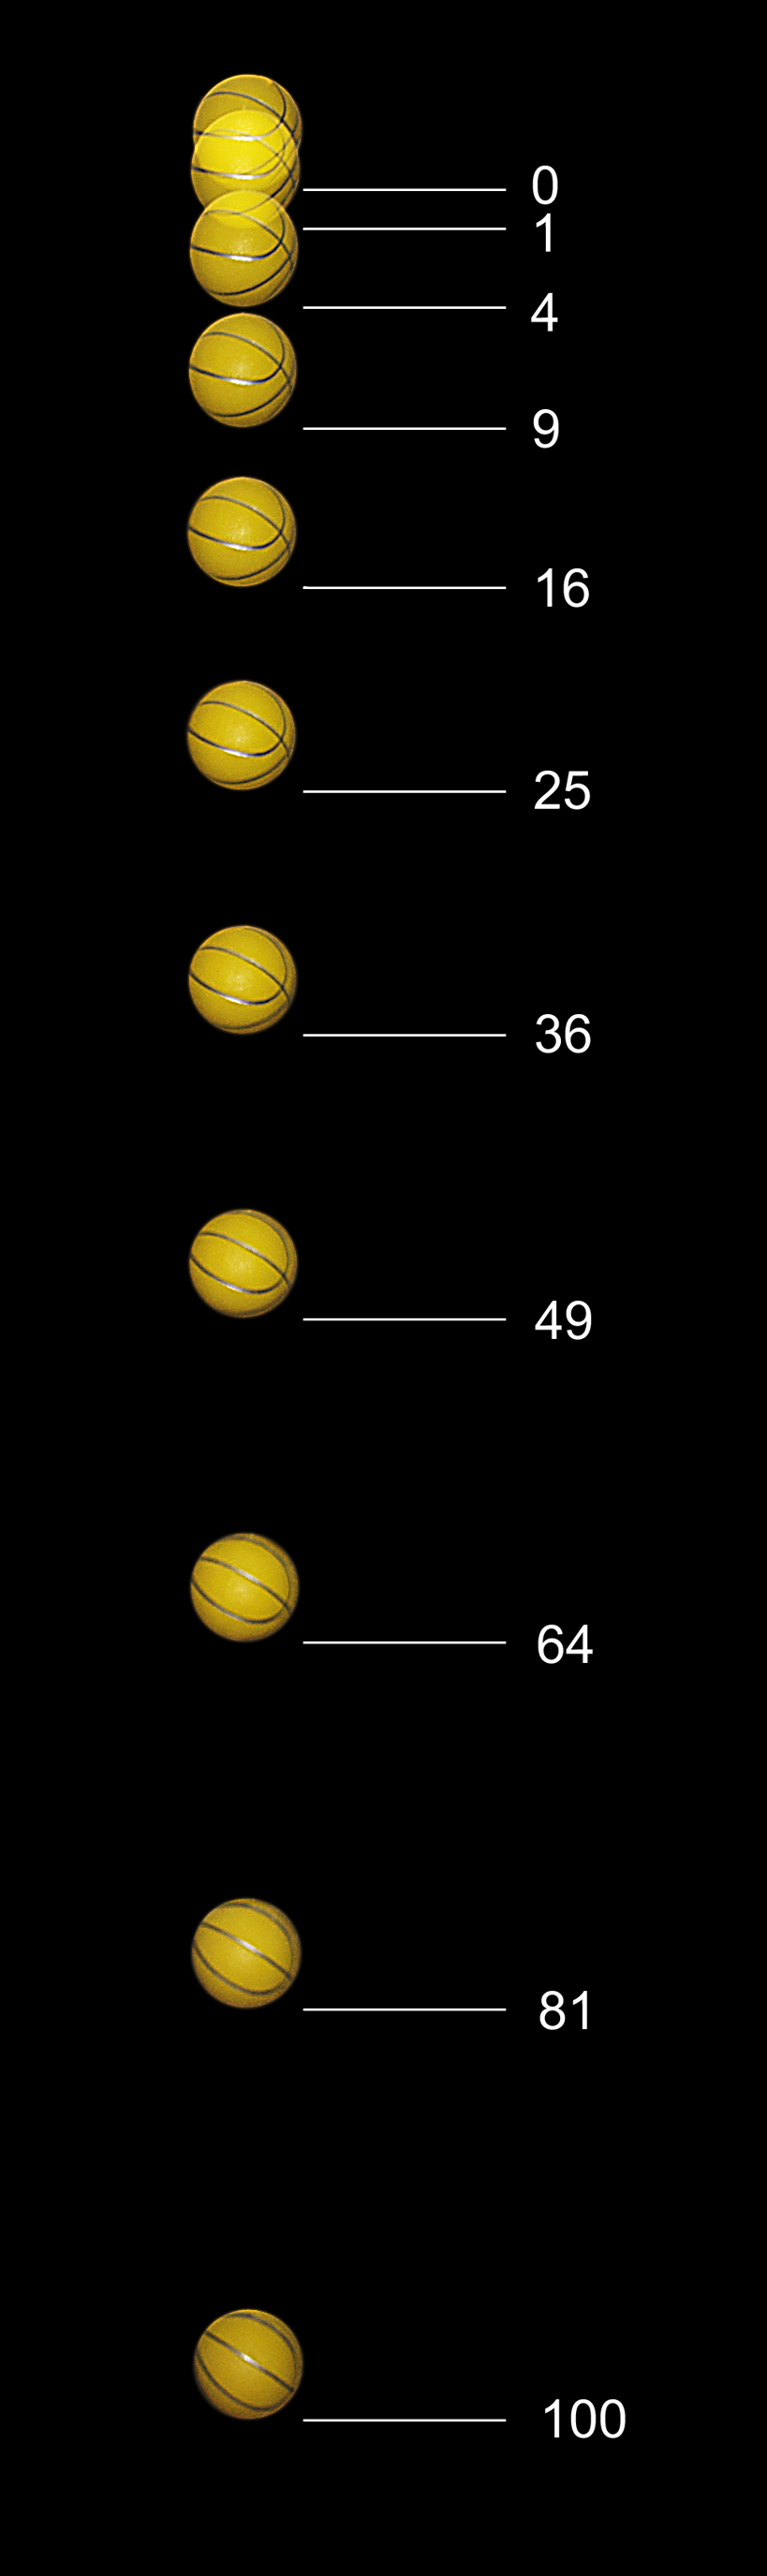
\includegraphics[width=0.15\textwidth]{00/fallingball.jpeg}
  };

\end{tikzpicture}}%
\only<1->{How can we use gravity to compute square roots?}

\only<2-3>{We know from physics}
\only<3->{
\begin{eqnarray*}
\only<3>{\ColorR{d} & = & \frac{1}{2} a \ColorG{t}^{2} \\}
\only<4->{\ColorG{t} & = & \sqrt{\frac{2\ColorR{d}}{a}}}
\end{eqnarray*}}
\only<5->{To compute $\sqrt{n}$, we just need to drop a ball from height $\ColorR{d}=\frac{an}{2}$ and measure the time for the ball to hit the ground.}
\only<6->{
\MedSkip{}
Example:
\begin{eqnarray*}
a & = & 9.8 \mbox{ m/$s^2$} \\
n & = & 81 \\
\ColorR{d} & = & an / 2 = 369.9 \mbox{ meters}
\end{eqnarray*}
Takes 9 seconds to drop}
\end{frame}

\begin{frame}{Using DNA to solve Traveling Salesperson\LinkArrow{https://www.jyi.org/2005-september/2005/9/7/fear-not-traveling-salesmen-dna-computing-is-here-to-save-the-day}}{Uses biophysical properties of ligation and electrophoresis}
    
\begin{columns}
    \begin{column}{0.5\textwidth}
        \begin{itemize}
            \item<1-> Each city is represented by a strand of DNA, with a unique first and last part.
            \item<2-> The strand of one city can ligate (attach) to the strand of an adjacent city, thus extending the path.
            \item<3-> These strands of DNA can be sorted by length using \href{https://en.wikipedia.org/wiki/Gel_electrophoresis}{electrophoresis}, with the shortest acceptable strand encoding the solution.
        \end{itemize}
 
    \end{column}
    \begin{column}{0.5\textwidth}  %%<--- here
     \begin{center}
        \vskip -2.5em
        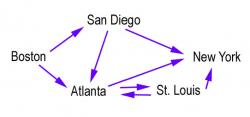
\includegraphics[width=0.7\textwidth]{00/map.jpeg}
     \end{center}
     \only<1->{
        \Vskip{-2em}
        \begin{tabular}{lcl}
            San Diego & = & \texttt{TTG AAA} \\
            Atlanta   & = & \texttt{TTT CTC}
        \end{tabular}
     }
     \only<2->{
        \MedSkip{}
        Possible ligation:
        
        \begin{tabular}{lll}
            \texttt{TTG} & \texttt{AAA} \\
               &  \texttt{TTT} & \texttt{CTC}
        \end{tabular}
     }
     
     \only<3->{
        \MedSkip{}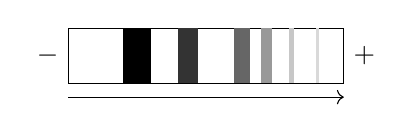
\begin{tikzpicture}[scale=0.7]
              \draw (0,0) rectangle(5,1);
              \node at (0,0.5) [left] {$-$};
              \node at (5,0.5) [right] {$+$};
              \draw[->] (0,-0.25) -- (5,-0.25);
              \fill[color=black!100!white] (1,0) rectangle(1.5,1);
              \fill[color=black!80!white] (2,0) rectangle(2.35,1);
              \fill[color=black!60!white] (3,0) rectangle(3.3,1);
              \fill[color=black!40!white] (3.5,0) rectangle(3.7,1);
              \fill[color=black!22!white] (4,0) rectangle(4.1,1);
              \fill[color=black!15!white] (4.5,0) rectangle (4.55,1);
        \end{tikzpicture}
     }
    \end{column}
\end{columns}

\end{frame}

\begin{frame}{Quantum effect}{Warning:  This material may be mind blowing}
\begin{itemize}
    \item Small particles such as electrons and photons live a very strange existence.
    \item We lack experience or even adequate language to understand and express how they behave.
    \item However, \href{https://en.wikipedia.org/wiki/Quantum_mechanics}{quantum mechanics} has been extraordinarily successful in predicting the outcomes of quantum events.
    \item Einstein did not (want to) believe that (his own) quantum theories were complete.\LinkArrow{https://en.wikipedia.org/wiki/Bohr-Einstein_debates}
\end{itemize}
\only<2->{
\begin{description}
    \item[Einstein:]  God does not play dice with the universe.
    \item[Bohr:] Don't tell God what to do with God's dice!
\end{description}}

\only<3->{\alert{
We can use quantum effects to compute interesting results.   In this course, we look at various problems and develop solutions based on quantum effects.}}

\end{frame}

\begin{frame}{Aside: physics theories}{What should they do for us?}
\begin{description}
    \item[predict outcomes]  The theory suffices when it predicts experimental results.  
    \begin{itemize}
        \item \href{https://en.wikipedia.org/wiki/Richard_Feynman}{Feynman} allegedly said \Quote{Shut up and calculate!}
        \item Perhaps he didn't say that. \LinkArrow{https://physicstoday.scitation.org/doi/10.1063/1.1768652}
        \item Maybe we should calculate but not be silent \LinkArrow{https://aeon.co/essays/shut-up-and-calculate-does-a-disservice-to-quantum-mechanics}
    \end{itemize}
    \item[explain stuff]  The theory should illuminate \emph{how} things work?
    \begin{itemize}
        \item What are the underlying mechanisms at work?
        \item What does this tell us about our world, how it was constructed, how it functions?
    \end{itemize}
\end{description}
This is an ongoing debate in physics.  We run into this problem studying how a ball flies through the air.  We can predict where it lands, but we cannot explain how gravity really works. 
\end{frame}
\begin{frame}{What are those quantum effects of interest to us?}{Superposition, interference, entanglement}
\begin{description}
    \item[Superposition:]  \only<1->{A quantum bit isn't necessarily in one state or another, but can be in a \emph{superposition} of states.  \only<1-3>{For example, consider a bucket of $r$~red and~$b$ blue marbles.  Until you draw a marble, the outcome is characterized as $r/(r+b)$ red $+$ $b/(r+b)$ blue.}}
    \only<2-3>{
    
    Once you draw from the bucket, that outcome has \emph{collapsed} to either fully red or fully blue.  
    
    Moreover, if you look at that drawn marble any number of times, it stays the same color.}
    
    
    \OnlyRemark{3}{
    In a quantum system, we can easily create the superposition of \emph{all} possible inputs to a function.}
    \only<4->{
    \item[Interference:]  In the superposition, we can influence the probability, up or down, of seeing a particular outcome using \emph{interference}.
    
    \only<4>{The effect here is akin to waves in a pool of water.   Based on their relative phases, two waves can pass through each other and either amplify or cancel each other.
    \Remark{We will use interference to emphasize the outcomes we wish to see.}
    }
    
    }
    \only<5->{
    \item[Entanglement:]  When two quantum bits are \emph{entangled}, their measurement outcomes are correlated, even if those outcomes are random.
    
    This is the most strange and useful property of quantum systems.  
    
    We will show that there is no information shared by such quantum bits that explains that behavior.
    
    
    }
\end{description}
\only<6>{\Example{We can entangle two quantum bits so that they randomly both measure either \True{} or \False{}, even if they are separated by light years from each other.}}

\only<7>{
\MedSkip{}Why do we care?  Harnessing these quantum effects allows us to solve some interesting problems in mere seconds that would take billions of years to solve on a classical computer.}
    
\end{frame}

\section{Logistics}

\begin{frame}{Course overview and logistics}{You are responsible for this knowledge}
The information is contained on this semester's \href{https://wustl.instructure.com/courses/80191/pages/overview-grading-academic-integrity?module_item_id=1145453}{canvas page}
\begin{itemize}
    \item Lecture
    \item Homework
    \item Exams
    \item Group work
    \item Academic integrity
    \item How to get help
\end{itemize}
\end{frame}

\begin{frame}{Course outline}{Subject to change}
\Vskip{-4em}\TwoColumns{%
\begin{enumerate}
    \item Introduction and background
    \item Reversible computations
    \item Computational complexity
    \item The physics
    \item Quantum systems
    \item Single qubit
    \item Universal quantum gates
    \item Elitzur--Vaidman bomb
    \item Beyond one qubit
    \item No-cloning theorem
    
\end{enumerate}
}{%
\begin{enumerate}
    \setcounter{enumi}{10}
    \item Quantum teleportation
    \item Quantum advantage
    \item Deutsch's problem
    \item Phase kickback trick
    \item Deutsch--Jozsa problem
    \item Simon's problem
    \item Bernstein--Vazirani problem
    \item Phase estimation
    \item Quantum Fourier
    \item Shor's algorithm
    \item Grover's algorithm
\end{enumerate}
}
    
\end{frame}

\SetTitle{1}{Background}{What you need to know}{01}

\section{Classical Logic}

\begin{frame}{Overview of classical logic}
\begin{itemize}
    \item You should be familiar with \href{https://en.wikipedia.org/wiki/Boolean_algebra}{Boolean algebra} but we will review it here.
    \item The two constants
    \begin{itemize}
        \item \Zero{} or \False{}
        \item \One{} or \True{}
    \end{itemize}
    \item We will review functions over those values.
    \item Classical logic uses \emph{bits} that are either \True{} or \False{}.
    \item Quantum logic uses \emph{qubits} that can be in a \emph{superposition} of \Zero{} and \One{}.
    \item We will study how to implement classical logic using quantum gates.
\end{itemize}
    
\end{frame}


\begin{frame}{Boolean functions of one input}
There are only two possible Boolean functions with just one input:
\begin{itemize}
    \item $f(x) = x$, the identity function
    \item $f(x) = \Not{x}$
\end{itemize}
The second function returns the \emph{complement} of the input value.  The operator is typically pronounced \emph{not}, and it is sometimes written $\neg x$.  In this class we prefer \Not{x}.

The truth table for this function is simple:
\begin{center}
\begin{tabular}{c|c}
$x$  & \Not{x} \\
\hline
\Zero{} & \One{} \\
\One{} & \Zero{} \\
\end{tabular}
\end{center}
\Remark{This function is \emph{reversible} and is its own inverse.}
    
\end{frame}

\def\BTable#1#2#3#4#5{%
\begin{center}
\begin{tabular}{cc|c}
$x$ & $y$ & \ensuremath{#1} \\
\hline
\Zero{} & \Zero{} & \ensuremath{#2} \\
\Zero{} & \One{} & \ensuremath{#3} \\
\One{} & \Zero{} & \ensuremath{#4} \\
\One{} & \One{} & \ensuremath{#5} \\
\end{tabular}
\end{center}
}
\begin{frame}{Boolean functions of two inputs}
For two inputs $x$ and $y$, we generally have:
\BTable{f(x,y)}{f(0,0)}{f(0,1)}{f(1,0)}{f(1,1)}
With four possible results, each \Zero{} or \One{}, there are $2^4$ possible tables. That is, 16 possible Boolean functions of two inputs.
\BigSkip{}
Some of those functions should be familiar.
\end{frame}

\begin{frame}{Conjunction and Disjunction}

\TwoColumns{
Conjunction

\BTable{x\wedge y}{0}{0}{0}{1}

The \emph{and} function is \True{} when both of its inputs are \True{}.

\only<2>{
We sometimes juxtapose inputs to imply conjunction:
\[x\wedge y = xy\]}
}{
Disjunction

\BTable{x\vee y}{0}{1}{1}{1}

The \emph{or} function is \True{} when either input is \True{}.

\only<2>{
We sometimes use $+$ as the operator for disjunction:
\[x\vee y = x + y \]}
}
\only<3>{
\Remark{These functions are \emph{not} reversible.  Even if we are given one of the inputs, the other input cannot be deduced from the output.}
}
\end{frame}

\begin{frame}{Exclusive or}{This operation is prevalent in quantum computations}

\BTable{\Xor{x}{y}}{0}{1}{1}{0}

Exclusive-or is what we usually mean in natural language when we say \emph{or}:
\MedSkip{}
\begin{quote}
    I am going to the gym or I am going to sleep.
\end{quote}
We mean we will do one or the other, but not both.
\Remark{
Given the output of this function and one of the inputs, we can deduce the value of the other input:
$\Xor{(\Xor{x}{y})}{x} = y$
}
\end{frame}

\begin{frame}{Universality}{Theoretically, what operators are needed at a minimum?}
\TwoColumns{
Consider again a general Boolean function of two inputs:
}{
\mbox{}\vskip -3em\mbox{}
\BTable{f(x,y)}{\alert<2>{r_{00}}}{\alert<3>{r_{01}}}{\alert<4>{r_{10}}}{\alert<5>{r_{11}}}
}
\MedSkip{}
Any of the 16 possible functions can be written as:
\[
f(x,y) = \visible<2->{\Not{x}\Not{y}\,r_{00}}\visible<3->{ +\Not{x}y \,r_{01} }\visible<4->{+ x\Not{y}\, r_{10} }\visible<5->{+xy \,r_{11} }
\]
For any $x,y$, exactly one of the above conjunctions involving $x$ and $y$ is true.  Thus, the above expression remains the same if $+$ is replaced by $\oplus$.  
\MedSkip{}
Based on the above, we see that universality is achieved using the three operators $\wedge$, $\vee$, $\neg$.
\end{frame}



\begin{frame}{Can we do better?}{Nand is a universal gate all by itself}
\TwoUnequalColumns{0.6\textwidth}{0.4\textwidth}{%
We define Nand as the not-of-and-of its two inputs:
\[ \Nand{x}{y} = \Not{xy} \]
}{%
\mbox{}\vskip -3.5em\mbox{}\BTable{\Nand{x}{y}}{1}{1}{1}{0}
}
\visible<2->{
\MedSkip{}
From this, we can compute the three operations that provide universality:
\begin{eqnarray*}
\Not{x} & = & \Nand{x}{1} \\
\And{x}{y} & = & \Not{\Nand{x}{y}} \\
\visible<3->{
\Or{x}{y} & = & \Nand{\Not{x}}{\Not{y}}}
\end{eqnarray*}
}
\visible<3->{
The last one follows from one of \href{https://en.wikipedia.org/wiki/De_Morgan\%27s_laws}{De~Morgan's laws}:
\[
\Not{uw} = \Or{\Not{u}}{\Not{w}}
\]
}
\visible<4->{
We can thus achieve universality with only a Nand gate.
}

\end{frame}

\section{Complex arithmetic}

\begin{frame}{Overview of complex arithmetic}
\begin{itemize}
    \item Complex arithmetic is especially convenient for quantum computing.
    \item We will use both forms:
    \begin{itemize}
        \item \href{https://en.wikipedia.org/wiki/Cartesian_coordinate_system}{Cartesian coordinates}
        \item \href{https://en.wikipedia.org/wiki/Polar_coordinate_system}{Polar coordinates}
    \end{itemize}
    \item Complex values allow us to express the magnitude of a wave as well as its phase.  This is helpful for understanding interference.
    \item We could defer using complex arithmetic in this course, but it is wise to embrace it from the start.
\end{itemize}
\end{frame}

\begin{frame}{Complex numbers}{Cartesian coordinates}
  
  \TwoColumns{%
  \begin{itemize}
     \item Each complex number $z$ has a \only<1->{\emph{real}} \only<2->{\emph{and an imaginary}} component.
     \item<3-> Point $z$ is expressed in the usual notation, with $\NiceI=\sqrt{-1}$
     \item<4-> The \emph{conjugate} \Conj{z} of $z$ is obtained by negating its imaginary part.
     
  \end{itemize}
  }{%
    \begin{TIKZP}[scale=0.7]
  \draw[<->] (-1, 0) -- (2.5, 0) node[right] {
    $\Re$ 
  };
  
  \draw (1, 4pt) -- (1, -4pt) node[below] {$a$} ;
  
  \visible<2->{
  \draw[<->] (0, -2.5) -- (0, 2.5) node[above] {$\Im$};
  
  \draw (-4pt, 2) -- (4pt, 2) node[left] {$b\ $} ;
  
  }
  \visible<3->{
  \draw[->] (0, 0) -- (1, 2) ;
  \TZPoint{1.05,2.05}{$z=a+b\NiceI$}{above right}
  
  }
  \visible<4->{
  \draw[->] (0, 0) -- (1, -2) ;
  \TZPoint{1.05,-2.05}{$\Conj{z}=a-b\NiceI$}{below right}
  }
\end{TIKZP}
}
\only<4->{\BigSkip{}The \emph{magnitude} of $z$ is given by $\Mag{z} =  \sqrt{a^{2}+b^{2}}$.}\only<5->{  We thus obtain:
\[
 \Mag{z}^{2}  =  a^{2}+b^{2} = z\Conj{z} = \Conj{z}z
\]
}
\end{frame}

\begin{frame}{The complex unit circle}{All points on the circle have unit length}

\TwoColumns{%
 \begin{itemize}
     \item<1-> The unit circle has radius~$1$.
     \item<2-> On the real axis, the circle has intercepts at~\only<2->{$+1$} \only<3->{and~$-1$.}
     \item<4-> On the imaginary axis, the circle has intercepts at~\only<4->{$+\NiceI$} \only<5->{and~$-\NiceI$.}
 \end{itemize}
 }{%
 \begin{TIKZP}[scale=1.3]
    \UnitComplexCircle{}
    \only<2->{\TZPEast{}}
   \only<4->{\TZPNorth{}}
   \visible<3->{\TZPWest{}}
   \only<5->{\TZPSouth{}}
    
 \end{TIKZP}}
 
 \only<5->{
 \BigSkip{}
 We typically express angles in radians in quantum computing, so the circle has $2\pi$ radians.  We proceed around the circle counterclockwise, beginning at point~$+1$.}

\end{frame}


\begin{frame}{From Cartesian to polar coordinates}
\TwoColumns{
\begin{itemize}
    \item<1-> A complex number $z$ as shown to the right is at the Cartesian coordinate
    \[z=\ColorOne{r}(\cos{\ColorTwo{\theta}}+\NiceI\sin{\ColorTwo{\theta}})\]
    \item<2-> From \href{https://en.wikipedia.org/wiki/Euler\%27s_formula}{Euler's formula}, we can write this using reals \ColorOne{$r$} and \ColorTwo{$\theta$} as
    \[ z = \Polar{\ColorOne{r}}{\ColorTwo{\theta}} \]
    
\end{itemize}
    
 }{%
  \begin{TIKZP}[scale=1.2]
    \UnitComplexCircle{}
    \draw[->,ultra thick] (1,0) arc (0:45:1) coordinate (z) ;
    \draw[thick] (0,0) -- (z) ;
    \TZText{0.5,0}{\ColorTwo{$\theta$}}{above}
    \TZText{z}{$z$}{above right}
    \TZText{0.35,0.35}{\ColorOne{$r$}}{above}
    \TZPoint{1,0}{$(\ColorOne{r},0)$}{below right}
 \end{TIKZP}
 }
 \only<3->{
\BigSkip{}The complex number \Polar{\ColorOne{r}}{\ColorTwo{\theta}} can thus be found by starting at $(\ColorOne{r},0)$ and walking counterclockwise around a circle of radius \ColorOne{$r$},
traversing a distance of \ColorTwo{$\theta$} radians along the circle.}
\end{frame}

\begin{frame}{Complex numbers in polar coordinates}{Useful properties}
\TwoColumns{%
Multiplication and Conjugation
\begin{itemize}
    \item<1-> Given $z_{1}=\Polar{\ColorOne{r_{1}}}{\ColorTwo{\theta_{1}}}$ and $z_{2}=\Polar{\ColorThree{r_{2}}}{\ColorFour{\theta_{2}}}$
    \item<2-> $z_{1}z_{2} = \Polar{\ColorOne{r_{1}}}{\ColorTwo{\theta_1}}\Polar{\ColorThree{r_{2}}}{\ColorFour{\theta_2}}$
    \item<3-> $z_1z_2 = \Polar{\ColorOne{r_{1}}\ColorThree{r_{2}}}{(\ColorTwo{\theta_1}+\ColorFour{\theta_2})}$
    \item<4-> Given $a=\Polar{r}{\theta}$, how do we find $\Conj{z}$?
    \item<4-> $\Conj{z} = \Conj{(\Polar{r}{\theta})}$
    \item<4-> $\Conj{z} = \Conj{r(\cos{\theta}+\NiceI\sin{\theta})}$
    \item<4-> $\Conj{z} = r(\cos{\theta}-\NiceI\sin{\theta})$
    \item<4-> $\Conj{z} = r(\cos(-\theta)+\NiceI\sin(-\theta))$
    \item<4-> $\Conj{z} = \Polar{r}{(-\theta)}$
\end{itemize}
}{
Magnitude
\begin{itemize}
    \item<5-> $\Forall{\theta}{\Mag{\ExpPhase{\theta}}=\sin^{2}\theta+\cos^{2}\theta=1}$
    \item<6-> $\Mag{r\ExpPhase{\theta}}=\Mag{r}\times\Mag{\ExpPhase{\theta}}=r$
    \item<7-> $\Implies{z=r\ExpPhase{\theta}}{\Mag{z}=\Mag{\Conj{z}}=r}$
    \item<8-> $\Implies{z=r\ExpPhase{\theta}}{\Mag{z\Conj{z}}=\Mag{\Conj{z}z}=r^{2}}$
\end{itemize}
}
    
\end{frame}

\section{Linear algebra}

\begin{frame}{Overview of linear algebra}{Quantum systems are linear!}
\begin{itemize}
    \item While much of our world behaves nonlinearly, quantum systems can surprisingly be captured using linear algebra.
    \item Vectors and matrices can represent states and gates.  
    \begin{itemize}
        \item The state of a quantum system is most often described as a column vector, called a \href{https://en.wikipedia.org/wiki/Bra-ket_notation}{ket}, such as $\QState{}=\PZero{}$.  More on this notation coming up$\ldots$
         \item The effect of a quantum gate can be described as a square matrix, which maps in input ket to an output ket.
    \end{itemize}
    \item This is convenient but not efficient in the number of quantum bits.
    \begin{itemize}
        \item A vector representing $k$ quantum bits has length $2^{k}$.
        \item A matrix describing a $k$-bit quantum gate has $2^{k} \times 2^{k}$ entries.
    \end{itemize}
    \item The composition of states and gates is computed using \href{https://en.wikipedia.org/wiki/Tensor}{tensor arithmetic}.
\end{itemize}
    
\end{frame}

\begin{frame}{Bra--ket notation}{Describing quantum states}
Quantum computing borrows notation from physics in using \href{https://en.wikipedia.org/wiki/Paul_Dirac}{Paul Dirac}'s \href{https://en.wikipedia.org/wiki/Bra-ket_notation}{bra--ket} notation.
\TwoColumns{%
\begin{itemize}
\item<1-> We typically represent a quantum state using a column vector.


\item<2-> Dirac calls such a vector a \emph{ket}, using this syntax that looks strange, but will soon become useful.


\end{itemize}
}{
\[
\visible<2->{\ket{\psi} = }
\begin{pmatrix}
.578\\ .408\NiceI \\ .319+.253\NiceI \\ -.578

\end{pmatrix}
\]
\visible<3->{The letter \alert{$\psi$} is typically used in quantum computing to represent \alert{p}state, and especially \alert{p}superpositions.}
}

\only<4->{\BigSkip{} The \emph{bra} of a ket is its conjugate transpose, and \VV{}.
\[
\bra{\psi} =
\begin{pmatrix}
.578 & -.408\NiceI & (.319-.253\NiceI) &  -.578
\end{pmatrix}
\]
}
\end{frame}

\begin{frame}{Inner Products}
The complete bra--ket of a state \QState{} is the inner product of its bra with the ket, which computes the magnitude of the state, squared:
\Vskip{-2em}\begin{eqnarray*}
\braket{\psi}{\psi} & = &
\begin{pmatrix}
\ColorOne{.578} & \ColorTwo{-.408\NiceI} & \ColorThree{(.319-.253\NiceI)} &  \ColorFour{-.578}
\end{pmatrix}
\times\begin{pmatrix}
\ColorOne{.578}\\ \ColorTwo{.408\NiceI} \\ \ColorThree{.319+.253\NiceI} \\ \ColorFour{-.578}
\end{pmatrix}
\\
 & = & \visible<2->{\ColorOne{.578^{2}}}  \visible<3->{\ColorTwo{-(.408\NiceI)^{2}}} \visible<4->{\ColorThree{+ (.102-.064\NiceI^{2})}} \visible<5->{\ColorFour{+ .578^{2}}} \\
\visible<6->{ & = & \Prob{\QState{}}}
\end{eqnarray*}%
\visible<7->{%
For a state~\QState{} that arises in a quantum system,  the above expression is expected to be~$1$.}\visible<8->{  The magnitude-squared of each component is the probability of observing its corresponding bit pattern on measurement.}\visible<9->{  In this example, we would see~\ColorOne{00} or~\ColorFour{11} with probability $\frac{1}{3}$}\visible<10->{, and see~\ColorTwo{01} or~\ColorThree{10} with probability $\frac{1}{6}$.}
\end{frame}


\section*{Outer products}

\begin{frame}{Outer products}
\begin{itemize}
    \item If we instead multiply a ket--bra pair, we obtain an \href{https://en.wikipedia.org/wiki/Outer_product}{outer product}.
    \item Outer products can be used to generate matrices from vectors.
    \item We look at two such uses of outer products:
    \begin{itemize}
        \item Building a gate using outer products, based on where we want to send basis vectors
        \item Decomposing an arbitrary matrix using outer products
    \end{itemize}
\end{itemize}
\end{frame}

\begin{frame}{Outer products of computational-basis vectors}{These generate a useful matrix}
\begin{itemize}[<+->]
    \item States of the computational basis are orthogonal.
    \item Thus, the \emph{inner product} \braket{i}{j} is either~$1$ or~$0$, if $i=j$ or $i\not=j$, respectively.
    \item Because \bra{i} and \ket{j} are one-hot vectors, the outer product \KetBra{i}{j} creates a matrix with a~$1$ in row~$i$ and column~$j$.  All other entries are~$0$.
    \item Example
    \[ \CDQB{0}{0}{0}{1}\DQB{0}{0}{1}{0} =\]
\end{itemize}
\end{frame}

\begin{frame}{Recalling the behavior of the computational basis}{A basis vector selects a given column or row of a matrix}
\begin{itemize}[<+->]
    \item Define \bra{i} as a \href{https://en.wikipedia.org/wiki/One-hot}{one-hot} vector, with a~$1$ in entry~$i$ and zeros elsewhere.  
    
    For example, in a 3-qubit system, $\bra{6} = (0\ 0\ 0\ 0\ 0\ 0\ 1\ 0)$.  
    
    In binary notation, this state is \bra{110}.
    \item Define \ket{i} similarly, as the analogous column vector.
    \item Consider an $n$-qubit system with an operator $U$: a $2^{n}\times 2^{n}$ matrix.
    \item Then $U\ket{i}$ returns column $i$ of $U$ by selection in the product.
    \item Example:
    \[ \CNOTMatrix\ket{2} = \CNOTMatrix\DQB{0}{0}{1}{0} = \DQB{0}{0}{0}{1}\]
    \item Similarly, $\bra{i}U$ returns row~$i$ of $U$.
\end{itemize}
\end{frame}

\begin{frame}{Building a gate using outer products}{An example: the \PauliX{} gate}

Suppose we want to build a quantum \emph{not} gate (Pauli \PauliX):
\begin{itemize}
    \item<2-> \ColorThree{\ket{0}} maps to \ColorOne{\ket{1}}
    \item<3-> \ColorThree{\ket{1}} maps to \ColorTwo{\ket{0}}
\end{itemize}
\visible<4->{A basis bra \ColorThree{\bra{i}} sends the preceding ket} \visible<5->{(below, \ColorOne{\ket{1}}} \visible<6->{and \ColorTwo{\ket{0}})}\visible<7->{ into column \ColorThree{$i$} of a matrix with all other entries $0$.}
\visible<4->{
\[\visible<5->{\ColorOne{\ket{1}}}\visible<4->{\ColorThree{\bra{0}}} + \visible<6,7,9->{\ColorTwo{\ket{0}}}\visible<4->{\ColorThree{\bra{1}}} = 
\visible<5->{\ColorOne{
\begin{pmatrix}
0 \\ 1
\end{pmatrix}}}
\visible<4->{\ColorThree{
\begin{pmatrix}
1 & 0
\end{pmatrix}}}
+
\visible<6,7,9->{\ColorTwo{
\begin{pmatrix}
1 \\ 0
\end{pmatrix}}}
\visible<4-7,9->{\ColorThree{
\begin{pmatrix}
0 & 1
\end{pmatrix}}}
\visible<8->{
= 
\begin{pmatrix}
\ColorOne{0} & 0 \\
\ColorOne{1} & 0
\end{pmatrix}}
\visible<9->{
+
\begin{pmatrix}
0 & \ColorTwo{1} \\
0 & \ColorTwo{0}
\end{pmatrix}}
\visible<10->{
=
\begin{pmatrix}
\ColorOne{0} & \ColorTwo{1} \\
\ColorOne{1} & \ColorTwo{0}
\end{pmatrix}
= \PauliX{}}
\]}
\only<11->{%

That column is then chosen by \ColorThree{\ket{i}} when subjected to the matrix:  $\PauliX(\ColorThree{\ket{0}})=\ColorOne{\ket{1}}$ and $\PauliX(\ColorThree{\ket{1}})=\ColorTwo{\ket{0}}$.}
\end{frame}

\section*{State vectors}

\begin{frame}{State vectors}{A column vector represents a state in quantum computing}

\TwoUnequalColumns{0.85\textwidth}{0.15\textwidth}{%
\Vskip{-3em}\begin{itemize}
    \item<1-> Quantum computing deals greatly with probability distributions among states.
    \item<2-> We use vectors to represent states, with an entry for every possible combination of observable outcomes.
    \item<3-> So, the state of an $n$-qubit system is represented by a vector of $2^n$ entries.  On the right is a $2$-qubit system with~4 combinations of observables \visible<4->{\ColorOne{$00$}}\visible<5->{, \ColorTwo{$01$}}\visible<6->{, \ColorThree{$10$}}\visible<7->{, and~\ColorFour{$11$}.}
    \item<8-> If the vector on the right contained probabilities, we would insist that they sum to~$1$.
    \item<9-> In quantum computing, the entries are not probabilities. They are \href{https://en.wikipedia.org/wiki/Probability_amplitude}{probability amplitudes}, which can be negative.  The \href{https://en.wikipedia.org/wiki/Square_(algebra)\#Absolute_square}{modulus square} of such a quantity yields the probability of the corresponding observable's outcome.
\end{itemize}%
}{%
\only<3->{%
\[\DQB{\visible<4->{\CFCirc{\RCone}}}{\visible<5->{\CFCirc{\RCtwo}}}{\visible<6->{\CFCirc{\RCthree}}}{\visible<7->{\CFCirc{\RCfour}}}\]
}%
}
\end{frame}

\begin{frame}{Unit vectors in quantum computing}{The discipline is based on the $2$-norm}

\TwoUnequalColumns{0.85\textwidth}{0.15\textwidth}{%
\only<1-5>{%
\Vskip{-3.5em}\begin{itemize}
    \item<1-> Consider a general vector shown to the right with $m$ entries.  
    \item<2-> The \href{https://en.wikipedia.org/wiki/Norm_(mathematics)\#p-norm}{$p$-norm} of a vector $v$ is defined as
    \Vskip{-1em}\[
    \PNorm{v}{p} = \left(\sum_{i=1}^{m} \Mag{x_{i}}^p\right)^{1/p}
    \]
    \item<3-> $p=1$ is the \href{https://en.wikipedia.org/wiki/Norm_(mathematics)\#Taxicab_norm_or_Manhattan_norm}{Manhattan norm}, the sum of a vector of distances.
    \item<4-> Quantum computing uses the \href{https://en.wikipedia.org/wiki/Norm_(mathematics)\#Euclidean_norm_of_complex_numbers}{$2$-norm} of a vector, requiring \ColorOne{unit length}:
    \[
    \Implies{\ColorOne{\sqrt{\sum_{i=1}^{m} \Prob{x_i}} = 1}}{\visible<5->{\ColorTwo{\sum_{i=1}^{m} \Prob{x_i}=1}}}
    \]
    \item<5-> With \Prob{x_i} as the probability of outcome~$i$, \ColorTwo{the above} requires that probabilities sum to~$1$.
\end{itemize}}%
}{%
\[
\QQB{x_1}{x_2}{x_3}{\SCirc{}}{\SCirc{}}{\SCirc{}}{\SCirc{}}{x_m}\]
}
\end{frame}

\begin{frame}{More on the $2$--norm}{From Scott Aaronson}

\begin{itemize}
\item 
\href{https://scottaaronson.com/}{Scott Aaronson} has said that much of the wonder of quantum computing can be attributed to its use of the 2-norm.\LinkArrow{https://www.scottaaronson.com/democritus/lec9.html}  That material is included in \href{https://www.amazon.com/Quantum-Computing-since-Democritus-Aaronson/dp/0521199565}{his book}.  

\item To me, he is the \href{https://en.wikipedia.org/wiki/Douglas_Hofstadter}{Douglas Hofstadter} of quantum computing.  I hope you enjoy reading their work as much as I do.
\item 
Let's follow his way of thinking about this \LinkArrow{https://www.scottaaronson.com/democritus/lec9.html} and see where it takes us.  This will take \alert{about 30~minutes}, and here are some helpful notes:
\begin{itemize}
    \item \href{https://en.wikipedia.org/wiki/Andrew_Wiles}{Andrew Wiles} is a mathematician who famously proved \href{https://en.wikipedia.org/wiki/Fermat\%27s_Last_Theorem}{Fermat's last theorem}. While that theorem concerns integer arithmetic, it poetically deals with squaring.
    \item \href{https://en.wikipedia.org/wiki/Raymond_Laflamme}{Ray Laflamme} is a quantum physicist with whom Aaronson \href{https://news.ycombinator.com/item?id=23621425}{worked in 2006} at \href{https://uwaterloo.ca/institute-for-quantum-computing/}{Waterloo's Institute for Quantum Computing}.
    \item \href{https://www.linkedin.com/in/ggutoski/}{Gus Gutoski} was a student in Aaronson's course.
\end{itemize}
\item Aaronson's views of the inherent interest in quantum computing are similar to \href{https://mitpress.mit.edu/contributors/richard-j-lipton}{Richard Lipton's}.
\end{itemize}

\end{frame}



\SetTitle{2}{Reversible computations}{No energy lost or gained}{02}

\begin{frame}{Overview}
\begin{itemize}
    \item Quantum computations involve gates that are \emph{unitary} and therefore are invertible.
    \item Quantum computations are delicate and noise must be kept to a minimum.  Interactions with the environment will cause the quantum system to collapse (\href{https://en.wikipedia.org/wiki/Quantum_decoherence}{decoherence}).
    \item We study a mechanical computer first where it is clear that a nonreversible computation gains or loses energy.
    \item We can build reversible circuits for classical and quantum computations.
    
\end{itemize}
\end{frame}

\section*{Reversible computations}

\begin{frame}{Reversible computing \LinkArrow{https://en.wikipedia.org/wiki/Reversible_computing}}{A brief history}
\begin{itemize}[<+->]
    \item A process that is reversible is \href{https://en.wikipedia.org/wiki/Isentropic_process}{isentropic}.
    \item This means that the system requires no net input of energy, and that it requires no net disposition of energy (such as heat loss).
    \item Long ago, such systems were \href{https://en.wikipedia.org/wiki/Charles_H._Bennett_(physicist)}{studied by scientists} because they had the potential to make computations more efficient.
    \item From a practical point of view, the energy lost by non-reversible computing is small compared to other energy losses in a computing system.
    \item However, quantum computing requires reversible gates.
    \item We begin with a mechanical example of an \NamedGate{and} gate, implemented using billiard balls.
\end{itemize}
\end{frame}


\begin{frame}{The \href{https://en.wikipedia.org/wiki/Billiard-ball_computer}{billiard ball computer}}{When a single ball enters at a time}
\TwoColumns{%
Consider the mechanical \NamedGate{and} gate shown here.
\begin{itemize}
    \item<1-> A ball entering from the top
    \only<2->{will emerge from the ``1-out'' hole.}
    \item<3-> A ball entering from the left
    \only<4->{will emerge from the ``0-out'' hole.}
    
\end{itemize}
}{%
\Vskip{-2em}\adjustbox{width=0.8\textwidth}{%
\begin{ReverseDiag}
\visible<1-2>{%
\visible<1>{\BBall{\RCone}{(1,1.5)}}
\draw<2>[->,ultra thick,dashed] (1,1.25) -- ++(0,-6.5);
\visible<2>{\BBall{\RCone}{(1,-5.75)}}}
\visible<3-4>{%
\visible<3>{\BBall{\RCtwo,}{(-1.75,-1.2)}}
\draw<4>[->,ultra thick,dashed] (-1.5,-1.2) -- ++(5.5,0);
\visible<4>{\BBall{\RCtwo,}{(4.5,-1.2)}}
}
\end{ReverseDiag}}

}
\visible<5->{
\MedSkip{}No energy is put in or taken out of the system.  The ball has its own energy, maintained throughout its motion through the box.}
    
\end{frame}

\begin{frame}{The \href{https://en.wikipedia.org/wiki/Billiard-ball_computer}{billiard ball computer}}{When two balls enter simultaneously}
\Vskip{-3em}\TwoUnequalColumns{0.55\textwidth}{0.45\textwidth}{%
Here, two balls enter simultaneously, \ColorOne{one from the top}, and \ColorTwo{one from the left}
\begin{itemize}
    \item<1-> The balls' first collision \visible<2->{is here.}
    \item<3-> They collide internally one more time.
    \item<4-> \ColorOne{One ball} emerges from the ``AND-output'' chute, \ColorTwo{the other} from the ``1-out'' chute.
    
\end{itemize}
}{%
\Vskip{-2em}\adjustbox{width=0.8\textwidth}{%
\begin{ReverseDiag}
\visible<1>{%
\BBall{\RCone}{(1,1.5)}
\draw[->,thick,\RCone] (1,1.5) -- ++(0,-2);
\BBall{\RCtwo,}{(-1.75,-1.2)}
\draw[->,thick,\RCtwo] (-1.75,-1.2) -- ++(2.5,0);}
\visible<2>{%
\BBall{\RCone}{(1,-0.5)}
\draw[->,thick,\RCone] (1,-0.5) -- ++(1.0,0) -- ++(0,-2);
\BBall{\RCtwo}{(0.5,-1.25)}
\draw[->,thick,\RCtwo] (0.5,-1.25) -- ++(0,-1.75) -- ++(1.25,0);
}
\visible<3>{%
\BBall{\RCone}{(2,-2.25)}
\draw[->,thick,\RCone] (2,-2.25) -- ++(2,0);
\BBall{\RCtwo}{(1.5,-3)}
\draw[->,thick,\RCtwo] (1.5,-3) -- ++(0,-2);
}
\visible<4->{%
\BBall{\RCone}{(4.5,-2.25)}
\BBall{\RCtwo}{(1.5,-5.5)}
}
\end{ReverseDiag}}
}
\visible<5->{
\MedSkip{}Again, the energy of the box remains the same throughout.\Remark{It would take energy to \emph{stop} the ball from exiting the ``1-out'' chute.}}

    
\end{frame}

\section{Reversible gates}
\begin{frame}{Not and And}{From page 12 of \Kaye{}}
\TwoColumns{%
\begin{itemize}
    \only<1>{
    \item The \emph{not} gate is reversible and is in fact its own inverse.}
    \item<2-> Is \And{a}{b} reversible if we know $a$?  \only<3->{\alert<3>{No}.} \only<3>{If $a=0$, $b$ could be either $0$ or $1$.}
    \item<4-> We need a copy of both inputs to create a reversible \emph{and} gate.
\end{itemize}
 
}{%


\begin{center}
\only<1>{
\begin{GateBox}[scale=0.5]{2}{1}{1}
\BoxLabel{Not}
\Input{0}{$a$}
\Output{0}{\Overline{a}}
\end{GateBox}}

\only<2-3>{\begin{GateBox}{2.5}{1}{2}
\BoxLabel{Reversible?}
\Input{0}{$a$}
\Input{1}{$b$}
\Output{0}{$a$}
\Output{1}{\And{a}{b}}
\end{GateBox}}


\only<4>{\begin{GateBox}{2.5}{1}{3}
\BoxLabel{Reversible?}
\Input{0}{$a$}
\Input{1}{$b$}
\Output{0}{$a$}
\Output{1}{$b$}
\Output{2}{\And{a}{b}}
\end{GateBox}}

\only<5>{\begin{GateBox}{2.5}{1.5}{3}
\BoxLabel{\mbox{\stackbox[c]{Reversible\\ And}}}
\Input{0}{$a$}
\Input{1}{$b$}
\Input{2}{\Zero{}}
\Output{0}{$a$}
\Output{1}{$b$}
\Output{2}{\And{a}{b}}
\end{GateBox}}
\end{center}
}
\MedSkip{}
   \only<4>{
    However, this box must generate energy to produce the third output.  To conserve energy, a reversible box must have the same number of inputs as outputs.}

\only<5>{This box enables reversal of the computation and it accepts an \href{https://en.wikipedia.org/wiki/Ancilla_bit}{ancilla} bit as a third input.}

\OnlyRemark{5}{The circuit elements involved in quantum computations must be \emph{reversible} and must contain the same number of inputs as outputs.}
\end{frame}

\begin{frame}{The Toffoli / CCNOT gate}{Uses the third input to greater advantage}
\TwoColumns{%
\begin{itemize}
    \item<1-> The signals $a$ and $b$ are copied to their respective outputs.
    \item<2-> The bottom output is computed as: 
    \only<2->{
    \Vskip{-2em}\begin{description}
        \item[$c=0$] The output is \And{a}{b}.
        \item[$c=1$] The output is \Nand{a}{b}.
    \end{description}}
    \item<2-> Because it can realize Nand, this reversible gate is \emph{universal} for constructing classical circuits.
    \item<3-> The gate is known in quantum computing as the \href{https://en.wikipedia.org/wiki/Toffoli_gate}{Tofolli Gate}.
\end{itemize}
}{%
\begin{center}
\begin{GateBox}{2.5}{1.5}{3}
\only<1-2>{\BoxLabel{\mbox{f(a,b)=\And{a}{b}}}}
\only<3-4>{\BoxLabel{Tofolli Gate}}
\only<5->{\BoxLabel{\mbox{\stackbox[c]{Tofolli Gate\\ CCNOT}}}}

\Input{0}{$a$}
\Input{1}{$b$}
\Input{2}{$c$}
\Output{0}{$a$}
\Output{1}{$b$}
\only<1-3>{\Output{2}{\Xor{c}{(\And{a}{b})}}}
\only<4->{\Output{2}{\Xor{(\And{a}{b})}{c}}}
\end{GateBox}
\end{center}
\only<4->{\MedSkip{}
An alternative view of this gate:
\begin{itemize}
    \item When $a$ and $b$ are both \True{}, the incoming signal $c$ is complemented on output.
    \item<5-> It is thus also called a controlled-controlled-Not gate, or CCNOT.
\end{itemize}
}
}
    
\end{frame}

\begin{frame}{CNOT gate}{Two-bit version of CCNOT}
\Vskip{-3em}
\TwoColumns{%

\begin{itemize}
    \item We can say $c$ controls whether the bottom output is $a$ or its complement.
    \item<2-> We prefer to say $a$ controls whether the bottom output is $c$ or its complement. This is \CNOT{a}{c}.
    \item<3-> The computation is reversible because
    $\Xor{a}{(\Xor{c}{a})} = c $.  \only<3>{We can thus recover $c$.}
    \item<4-> Here you see the quantum circuit symbol for \CNOT{a}{c}:  $a$ conditionally complements $c$.
\end{itemize}
}{%
\begin{GateBox}{2}{1}{2}
\BoxLabel{CNOT}

\Input{0}{$a$}
\Input{1}{$c$}
\Output{0}{$a$}
\Output{1}{\Xor{a}{c}}
\end{GateBox}
\begin{center}
\begin{tabular}{cc||cc}
\multicolumn{2}{c}{Inputs} &
\multicolumn{2}{c}{Outputs} \\
$a$ & $c$  & $a$ & \Xor{c}{a} \\ \hline
0 & 0 & 0 & 0 \\
0 & 1 & 0 & 1 \\
1 & 0 & 1 & 1 \\
1 & 1 & 1 & 0
\end{tabular}
\end{center}

\only<4->{
\begin{center}
\begin{quantikz}
\lstick{$a$} & \ctrl{1} & \qw & \rstick{$a$}\\ 
\lstick{$c$} & \targ{}  & \qw & \rstick{\Xor{a}{c}}
\end{quantikz}
\end{center}
}
}
\end{frame}

\begin{frame}{Generally reversible computation}{From \Kaye{} page 14}
\Vskip{-4em}\begin{center}
\begin{Pixture}[width=0.7\textwidth]{02}{kayep14fig1.6.png}
\end{Pixture}\end{center}
    
\end{frame}

\SetTitle{3}{Overview of computational complexity}{Review}{03}

\section{Overview}

\begin{frame}{Modeling computation}{Turing machines and complexity classes}
\begin{itemize}
    \item A \href{https://en.wikipedia.org/wiki/Turing_machine}{Turing machine} is a simple conceptual device that formalizes the state-to-state nature of computation.
    \item Nobody really builds such a machine, but we say that anything that is computable can be computed on a Turing machine.   
    \only<2>{
    \SmallSkip{}
    Well some people do build such machines:
    \begin{itemize}
        \item \href{https://www.youtube.com/watch?v=E3keLeMwfHY}{Using 35mm film}
        \item \href{https://www.youtube.com/watch?v=5_Hj5x6OWTM}{One with a connection to Washington University.}
    \end{itemize}}
    \item<3-> Here we can think of computation as a program we write. \only<3>{We have to make sure the language we use is clear about how many steps a given statement takes.}
    \item<4-> We can then talk about the number of steps it takes to solve a problem of some size~$n$.  You should already be familiar with \href{https://en.wikipedia.org/wiki/Asymptotic_computational_complexity}{asymptotic notation to express complexity}, especially the time an algorithm or problem takes.
\end{itemize}

\OnlyRemark{5}{We use asymptotic complexity to describe the time and area needed for computations on a quantum computer.}
    
\end{frame}

\section*{Unstructured search}

\begin{frame}{What input provides a given output?}{An interesting problem to consider}

\TwoColumns{%
\begin{center}

\only<1-2,5->{
\begin{GateBox}{2.5}{1}{1}
\BoxLabel{$f(x)$}
\Input{0}{$x$}
\Output{0}{$y$}

\end{GateBox}
}
\only<3-4>{
\begin{GateBox}{2.5}{1}{1}
\BoxLabel{$f(x)=2x+5$}
\Input{0}{?}
\Output{0}{105}

\end{GateBox}
}

\end{center}
\SmallSkip{}
\begin{itemize}
    \item<1-> What input value for $x$ produces a $y$ of interest?
    \item<2-> Given the inverse of $f$, we could compute $x=f^{-1}(y)$
    \item<5-> Not all functions are invertible.
    \item<6-> Some functions may take a long time to find (an) $x\ |\ f(x)=y$.
    
\end{itemize}
}{
\only<3-4>{%
\begin{itemize}
    \item<3-> Consider the function \[ f(x)=2x+5\]
    \item<4> We can use algebra to compute $x=50$ when $f(x)=105$.
\end{itemize}
}%
\only<5>{
\begin{itemize}
\item The function
\[ f(x)=x^{2} \] is \emph{not} invertible, because each output has two possible inputs.  
\item
Here, we can easily find an input that matches a given output, but we cannot hope to create a function $f^{-1}(y)$.
\end{itemize}
}
\only<6->{
\Vskip{-3em}\begin{itemize}
\item<6-> Examples of this include 
\begin{itemize}
    \item \href{https://en.wikipedia.org/wiki/Bitcoin}{Bitcoin}
    \item \href{https://en.wikipedia.org/wiki/SHA-1}{SHA-1}
    \item \href{https://en.wikipedia.org/wiki/MD5}{MD5}
    \item and other similar hash functions
\end{itemize}

\item<7-> This is an example of \emph{unstructured search}, which we examine next.  Quantum computers are asymptotically faster at solving such problems, but the speedup is relatively modest.
\item<8-> An asymptotically more impressive problem is \emph{factoring}, considered after that.
\end{itemize}
}

}
\end{frame}

\begin{frame}{Needle in an unstructured haystack}{The complexity of unstructured search}
\TwoColumns{%
\begin{itemize}
    \item Consider a Boolean-valued function $f(x)$ over domain \Domain{D}, $\Mag{\Domain{D}}=2^{n}$.
    \item For one special element $\SpecialX{x}\in\Domain{D}$, $f(\SpecialX{x})=\True$.
    \item $\Forall{x \not= \SpecialX{x}}{f(x)=\False{}}$.
    \item<3-> For analysis, let $N=2^{n}$, and we assume \Domain{D} has no structure to guide a search.
\end{itemize}

}{%
\only<2>{%
Some examples:
\begin{itemize}
    \item $n$ two-position switches
    \item A \href{https://en.wikipedia.org/wiki/Combination_lock\#Single-dial_locks}{combination lock} with a dial of integers $1\ldots 2^{n/3}$.
    \begin{itemize}
        \item The input consists of three integers, each  a position on the dial.
        \item The total number of combinations is then $\left(2^\frac{n}{3}\right)^3=2^{n}$.
    \end{itemize}
\end{itemize}}%
\only<4->{%
How much time does it take to find \SpecialX{x}?
\begin{itemize}
    \item<4-> Classically, the best we can do is $\Theta(N)$, average- and worst-case.
    \item<5-> If we use $p$ processors, this becomes $\Theta(N/p)$, but unless $p$ scales with $N$, the complexity is unimproved.
    \item<6-> As we will study, \href{https://en.wikipedia.org/wiki/Grover\%27s_algorithm}{Grover's algorithm} offers a quantum computing solution taking $\Theta(\sqrt{N})$ time.
\end{itemize}}
}
\OnlyRemark{7}{Consider how \emph{you} would achieve such a bound looking for something.  The quantum world is strange but offers the promise of greater computing power.}
\end{frame}


\section{Factoring}

\begin{frame}{The factoring problem}{Given an integer $n$, find integers $p$ and $q$ such that $pq=n$}
\TwoColumns{%

\begin{itemize}
    \item We don't know yet the true difficulty of this problem.
    \item Classically, there is as yet no polynomial-time algorithm for solving this problem.
\item<5->
As we will study, a quantum computer can solve this problem in \alert{polynomial time} using \href{https://en.wikipedia.org/wiki/Shor\%27s_algorithm}{Shor's algorithm}.
\item<6> \emph{Aside}: do you see a familiar (to my class) 3-digit number embedded in each of the factors?
\end{itemize}
}{
\begin{itemize}
    \item Can you factor 21 easily into its two prime factors?  \only<2->{$21=7\times 3$}
    \item<3-> How about \[329716591508669867994509609\]
    \item<4-> It is the product of the \href{https://en.wikipedia.org/wiki/Pell_number\#Primes_and_squares}{Pell prime} \[1746860020068409\]
    and the \href{https://en.wikipedia.org/wiki/Wieferich_prime}{Wieferich prime} \[188748146801\]
    
\end{itemize}
}
\end{frame}


\begin{frame}{The discrete log problem}{\href{https://en.wikipedia.org/wiki/Diffie\%E2\%80\%93Hellman_key_exchange}{Key exchange protocol} for \href{https://en.wikipedia.org/wiki/HTTPS}{\texttt{https}}}
\TwoColumns{%
Consider the function
\only<1-2>{
\[ y = g^{x} \bmod p \]
}%
\only<3->{
\[ y = 3^{x} \bmod 17 \]
}%
\visible<1-2>{%
for integers $x, y, g, p$.  Typically $p$ is a very large prime.}
\only<2->{
\begin{itemize}
    \item<2-> Consider $g=3$ and $p=17$
    \item<4-> Suppose $y=13$, what is $x$?
    \item<5-> $x=4$ works
\end{itemize}
}
}{%
\begin{itemize}
    \item Who knows what?
    \begin{itemize}
    \item The world knows $g$ and $p$.
    \item $x$ is private
    \item $y$ is public
    \end{itemize}
    \item Computing $y$ from $x$ is easy and efficient.
    \item Computing $x$ given $y$ is considered difficult classically.
\end{itemize}
}
\OnlyRemark{6}{%
The problem of finding $x$ given $y$ is the \href{https://en.wikipedia.org/wiki/Discrete_logarithm}{discrete logarithm} problem.
}
    
\end{frame}

\begin{frame}{Diffie--Hellman key exchange}{Secrecy relies on the apparent difficulty of discrete log}

\Vskip{-3em}\begin{ProtocolDialog}{0.28\textwidth}{0.33\textwidth}{0.37\textwidth}
\visible<2->{\All{$g=5$ and $p=23$.}{My secret $a=7$.}{My secret $b=12$.}}
\visible<3->{\All{Compute $5^{x}\bmod 23$}{I compute $A=5^{a}\bmod 23$.}{I compute $B=5^{b}\bmod 23$.}}
\visible<4->{\All{Publish the result}{I publish $A=17$.}{I publish $B=18$.}}
\visible<5->{\All{Everybody hears $Y$}{$B=18$}{$A=17$.}}
\visible<6->{\All{{\small Compute} $Y^{x} \bmod 23$}{I compute $B^{a}\bmod 23$.}{I compute $A^{b}\bmod 23$.}}
\visible<7->{\All{}{I obtain $6=18^{7}\bmod 23$.}{I obtain $6=17^{12}\bmod 23$.}}
\visible<8->{\All{They agree!}{We have a shared key $6$.}{We have a shared key $6$.}}
\end{ProtocolDialog}
\OnlyRemark{9}{%
It's easy to compute $A$ from $a$ and $B$ from $b$.  There is no known \emph{efficient} classical algorithm for computing $a$ given $A$ and $B$.  Alice and Bob share the key and nobody else can compute it efficiently unless they know $a$ or $b$---unless they have a sufficiently large quantum computer.
}
    
\end{frame}

\begin{frame}{Summary}{And why should you study quantum computing?}

\begin{itemize}
    \item Computer scientists view problems and their algorithmic solutions through the lens of computational complexity.
    \item We have seen some problems here for which there are (as yet) no efficient algorithms for solving those problems on a classical computer.
    \item We will study quantum computing approaches to solving those problems efficiently.
    \item So$\ldots$why study quantum computing?
    \begin{itemize}
        \item Quantum mechanics allows us to reason about the behavior of small particles.
        \item Such behavior can be leveraged to compute useful information.
        \item We have examples of problems that appear to be very difficult on a classical computer but which have efficient solutions on a quantum computer.
    \end{itemize}
\end{itemize}
    
\end{frame}

\section*{Quantum puzzles}

\begin{frame}{Quantum fly trap games and puzzles}{In preparation for next lecture}

\begin{itemize}
    \item \href{https://quantumflytrap.com/}{Quantum fly trap} is by Piotr Magdal, Klem Jankiewicz, and Pawel Grabarz \LinkArrow{https://quantumflytrap.com/about/}.
    \item \href{https://github.com/stared/quantum-game}{An older version} (no longer live) of this game was developed by Piotr Magdal.
    \item The \href{https://quantumflytrap.com}{newer version} adds useful features.
    \begin{itemize}
    \item \href{https://lab.quantumflytrap.com/game}{Here} are challenges with increasing difficulty, and you unlock higher levels by solving lower ones.
    \item \href{https://lab.quantumflytrap.com/lab}{Here} is the virtual lab where you can create and execute your own scenarios of interest.  
    \item Help on a component can be found by right-clicking on the component in the menu.
    \end{itemize}
    \item \alert{Get as far as you can and you can with \href{https://lab.quantumflytrap.com/game}{the challenges} and perhaps present your solutions in class next time.}
\end{itemize}
    
\end{frame}



\SetTitle{4}{The physics}{Becoming a believer}{04}

\section{Overview}
\begin{frame}{Overview}{What will we study here?}
\begin{itemize}
    \item We have some experience with polarized light, so we begin by investigating some theories about how a succession of polarizing filters behaves.  This will serve as our introduction to \href{https://en.wikipedia.org/wiki/Quantum_superposition}{superposition}.
    \item We must look at the classic \href{https://en.wikipedia.org/wiki/Double-slit_experiment}{double-slit} experiment which involves both superposition and \href{https://en.wikipedia.org/wiki/Wave_interference}{wave interference}.
    \item We return to polarized light by playing some \href{https://lab.quantumflytrap.com/lab}{quantum games} (older site \href{http://play.quantumgame.io/}{here}).
\end{itemize}
    
\end{frame}
\section{Polarized light}

\begin{frame}{Polarized light}{Experiments you can do with commonly found polarizing filters}
\begin{itemize}
    \item The experiments described here can be carried out using \href{https://en.wikipedia.org/wiki/Polarizer}{polarizers}.
    \item Examples include
    \begin{description}
        \item[sunglasses] These are polarized to diminish reflected light from surfaces such as water.  Such light is typically polarized horizontally, so these sunglasses admit only vertically polarized light.
        \item[computer screen]  If you are watching these slides on an \href{https://en.wikipedia.org/wiki/Liquid-crystal_display}{LCD computer screen}, the light reaching your eyeballs is (most likely) linearly polarized.
    \end{description}
    \item You can thus do these experiments with your computer screen and $2-3$ pairs of polarizing sunglasses.
    
\end{itemize}
\OnlyRemark{2}{In the slides that follow, light is emitted from the screen and heading toward you.    Each successive filter is placed in front of the previous one.}
\end{frame}

\begin{frame}{A bad theory for polarization}{Based on the classical world}
\TwoUnequalColumns{0.65\textwidth}{0.35\textwidth}{%
\Vskip{-3em}\begin{itemize}
    \item<1-> Light is a collection of waves, each due to one \href{https://en.wikipedia.org/wiki/Photon}{photon}.
    \item<2-> Unpolarized light might then be many photons, each with an arbitrary angle of polarization.
    \item<3-> What happens when the photons strike a filter as shown here?
    \item<4-> Only those waves polarized vertically, or nearly so, would pass through. 
\end{itemize}
}{%
\only<2->{%
\Vskip{-3em}\begin{center}
\begin{TIKZP}
\RadiantArrows{22.5}{->,color=BrickRed,thick}
\end{TIKZP}
\end{center}
}%
\only<3->{%
\begin{center}
\begin{TIKZP}[overlay]
\PFilter{-1}{0.0}{1}{2.5}{20}
\end{TIKZP}
\end{center}
}%
\only<4->{%
\begin{center}
\begin{TIKZP}[scale=0.5]

  \draw[<->,thick,color=BrickRed] (0,-1) -- (0,1);

\end{TIKZP}
\end{center}
}
}
\OnlyRemark{5}{If this is true, we should see a very small fraction of the light passing through. But we see $\frac{1}{2}$ of the light passing through.  How can this be?}
\end{frame}

\begin{frame}{Polarizing filters in succession}{Observations about this experiment}
\TwoColumns{%
\begin{itemize}
    \item<1-> Start with unpolarized light.
    \item<2-> Impose a \textcolor{\RCtwo}{vertically polarizing filter}.
    \item<3-> You see half of the light passing through.
    \item<4-> Impose a second \textcolor{\RCthree}{identical filter}.
    \item<5-> No more light is filtered out this time.
    \item<6-> Impose \textcolor{\RCone}{another filter} at \Degrees{45}.
    \item<7> You now see half of the previous light passing through, now polarized according to this \textcolor{\RCone}{last filter}.
\end{itemize}
}{%
\begin{center}
\begin{TIKZP}
\visible<1-2>{\RadiantArrows{22.5}{->,color=BrickRed,thick}}
\visible<2>{\begin{scope}[draw=\RCtwo]\PFilter{-1}{-1.2}{1}{1.2}{20}\end{scope}}
\visible<3-4,5,6>{%
\foreach \x in {-1, -0.75,...,1} {
\draw[<->,thick,color=BrickRed] (\x,-1) -- (\x,1);
}
}
\visible<4>{\begin{scope}[draw=\RCthree]\PFilter{-1}{-1.2}{1}{1.2}{20}\end{scope}}

\visible<6>{\begin{scope}[draw=\RCone,rotate=45]\PFilter{-1}{-1.2}{1}{1.2}{20}\end{scope}}
\visible<7>{%
\begin{scope}[rotate=45]
\foreach \x in {-1, -0.5,...,1} {
\draw[<->,thick,color=BrickRed] (\x,-1) -- (\x,1);
}
\end{scope}
}
\end{TIKZP}
\end{center}
}
\end{frame}



\begin{frame}{Orthogonal filters}{They can eliminate all of the light}
\TwoColumns{%
\begin{itemize}
    \item<1-> Start with unpolarized light.
    \item<2-> Impose a \textcolor{\RCtwo}{vertically polarizing filter}.
    \item<3-> You see half the light passing through.
    \item<4-> Add a second \textcolor{\RCthree}{identical filter}, behind the first one, rotated \Degrees{90}.
    \item<5-> No light passes through now.  We should expect this.
\end{itemize}
}{%
\begin{center}
\begin{TIKZP}
\visible<1-2>{\RadiantArrows{22.5}{->,color=BrickRed,thick}}
\visible<2,4>{\begin{scope}[draw=\RCtwo]\PFilter{-1}{-1.2}{1}{1.2}{20}\end{scope}}
\visible<3-4>{%
\foreach \x in {-1, -0.75,...,1} {
\draw[<->,thick,color=BrickRed] (\x,-1) -- (\x,1);
}
}
\visible<4>{\begin{scope}[draw=\RCthree,rotate=90]\PFilter{-1}{-1.2}{1}{1.2}{20}\end{scope}}
\end{TIKZP}
\end{center}
}
\end{frame}

\begin{frame}{How much light passes through two filters?}{Getting quantitative}
\TwoUnequalColumns{.70\textwidth}{.30\textwidth}{%
\begin{itemize}
    \item<1-> When the filters align, so the angle between them is~\Degrees{0}, there is no change in the light passed through the second filter.
    \item<2-> When the filters are orthogonal, so the angle between them is~\Degrees{90}, no light passes through the second filter.
    \item<3-> If you experiment with various angles and measure the fraction of light that enters the first filter and passes through the second, you will see that it is related to $\cos^{2}\theta$, where $\theta$ is the angle between the filters' relative orientations.\LinkArrow{https://en.wikipedia.org/wiki/Polarizer\#Malus's_law_and_other_properties}
\end{itemize}
}{%
\begin{center}
\begin{TIKZP}
\visible<1-3>{\begin{scope}[draw=\RCtwo,rotate=90]\PFilter{-1}{-1.2}{1}{1.2}{20}\end{scope}
\draw[->,thick] (0,0) -- (1,0) ;
}
\visible<2>{\begin{scope}[draw=\RCthree]\PFilter{-1}{-1.2}{1}{1.2}{20}\end{scope}
\draw[->,thick] (0,0) -- (1,0) ;
\draw[->,thick] (0,0) -- (0,1);
}
\visible<3>{\begin{scope}[draw=Sepia,rotate=-20]\PFilter{-1}{-1.2}{1}{1.2}{20}\end{scope}
\draw[->,thick] (0,0) -- (70:1);
\draw (0.2,0) node[above right] {$\theta$};
}
\end{TIKZP}
\end{center}
}
\end{frame}

\begin{frame}{And now a surprise}{A filter can actually cause light to emerge}
\TwoUnequalColumns{0.65\textwidth}{0.35\textwidth}{%
\begin{itemize}
    \item<1-> Start with unpolarized light
    \item<2-> Impose a \textcolor{\RCtwo}{vertically polarizing filter}.
    \item<3-> You see half the light passing through.
    \item<4-> Add a second \textcolor{\RCthree}{identical filter}, in front the first one, rotated \Degrees{90}.
    \item<5-> You see no light, like previously.
    \item<6-> Impose \textcolor{\RCone}{another filter} at \Degrees{45} sandwiched \emph{between} the \textcolor{\RCtwo}{first} and \textcolor{\RCthree}{second} filters.
    \item<7> You now see 25\% of the light passing through and it is polarized according to the \textcolor{\RCthree}{last} filter.
\end{itemize}
}{%
\begin{center}
\begin{TIKZP}
\visible<1-2>{\RadiantArrows{22.5}{->,color=BrickRed,thick}}
\visible<2,4,6,7>{\begin{scope}[draw=\RCtwo]\PFilter{-1}{-1.2}{1}{1.2}{20}\end{scope}}
\visible<3-4>{%
\foreach \x in {-1, -0.75,...,1} {
\draw[<->,thick,color=BrickRed] (\x,-1) -- (\x,1);
}
}
\visible<6,7>{\begin{scope}[draw=\RCone,rotate=45]\PFilter{-1}{-1.2}{1}{1.2}{20}\end{scope}}
\visible<4,6,7>{\begin{scope}[draw=\RCthree,rotate=90]\PFilter{-1}{-1.2}{1}{1.2}{20}\end{scope}}
\visible<7>{%
\begin{scope}[rotate=90]
\foreach \x in {-0.5,0, ...,0.5} {
\draw[<->,thick,color=BrickRed] (\x,-1) -- (\x,1);
}
\end{scope}
}

\end{TIKZP}
\end{center}
}
\end{frame}

\begin{frame}{Quantum interpretation}{A theory that yields precise measurements}
\begin{itemize}
    \item An unpolarized photon is in a \emph{superposition} of polarizations.  Because our personal experiences differ so greatly from that of the photon, we lack the language to describe its behavior.  We will express this concept mathematically, as a linear combination of possible outcomes.  Here we can say that each outcome is equally likely.
    \item When the photon hits the polarizing filter, it interacts with the filter so as to either pass through or not.
    \begin{itemize}
        \item In the \href{https://en.wikipedia.org/wiki/Copenhagen_interpretation}{Copenhagen interpretation}, we say that the superposition \emph{collapsed} by this interaction, which constituted a \emph{measurement}.
        \item In the \href{https://en.wikipedia.org/wiki/Many-worlds_interpretation}{Many Worlds} interpretation, we became entangled with the measurement outcome we saw.  There is a different world where we saw the measurement turn out the other way.
    \end{itemize}
    \item The outcome is consistent with any number of subsequent, identical measurements.
    
\end{itemize}
\end{frame}

\begin{frame}{Reinterpretation of the surprise}{We have to analyze the effects of each filter in turn}
\TwoUnequalColumns{0.65\textwidth}{0.35\textwidth}{%
\begin{itemize}
    \item<1-> Start with unpolarized light
    \item<2-> Impose a \textcolor{\RCtwo}{vertically polarizing filter}.
    \item<3-> You see half the light passing through.
.
    \item<4-> The \textcolor{\RCone}{another filter} at \Degrees{45} sandwiched is next.
    \item<5-> Its angle will cause $\cos^2(\pi/4)=1/2$ of the light to pass through.
        \item<6-> Add the final filter \textcolor{\RCthree}{identical filter}, rotated \Degrees{90}.
    \item<6-> Its angle with the previous filter is also \Degrees{45}, so that the light is cut down by another factor of 2.
    
    \item<7> You thus see $1/4$ of the original light, polarized according to the \textcolor{\RCthree}{last} filter.
\end{itemize}
}{%
\begin{center}
\begin{TIKZP}
\visible<1>{\RadiantArrows{22.5}{->,color=BrickRed,thick}}
\visible<2->{\begin{scope}[draw=\RCtwo]\PFilter{-1}{-1.2}{1}{1.2}{20}\end{scope}}
\visible<2-3>{%
\foreach \x in {-1, -0.75,...,1} {
\draw[<->,thick,color=BrickRed] (\x,-1) -- (\x,1);
}
}
\visible<4->{\begin{scope}[draw=\RCone,rotate=45]\PFilter{-1}{-1.2}{1}{1.2}{20}\end{scope}}
\visible<4-5>{%
\begin{scope}[rotate=45]
\foreach \x in {-0.5,-0.25,...,0.5} {
\draw[<->,thick,color=BrickRed] (\x,-1) -- (\x,1);
}
\end{scope}}
\visible<6->{\begin{scope}[draw=\RCthree,rotate=90]\PFilter{-1}{-1.2}{1}{1.2}{20}\end{scope}}
\visible<6-7>{%
\begin{scope}[rotate=90]
\foreach \x in {-0.5,0.5} {
\draw[<->,thick,color=BrickRed] (\x,-1) -- (\x,1);
}
\end{scope}
}

\end{TIKZP}
\end{center}
}
\end{frame}

\section{Double-slit experiment}

\begin{frame}{Double-slit experiment}
\begin{itemize}
\item No introduction to quantum behavior is complete without some coverage of the \href{https://en.wikipedia.org/wiki/Double-slit_experiment}{double-slit experiment}.  

\item Let's look at (some of) \href{https://en.wikipedia.org/wiki/Umesh_Vazirani}{Umesh Vazirani}'s videos on this subject.
\begin{itemize}
    \item \href{https://www.youtube.com/watch?v=1X7CDd1lvR0}{Video 1} (7.5 minutes)
    \item \href{https://www.youtube.com/watch?v=pHmRp2eGETk}{Video 2} (13 minutes)
    \item \href{https://www.youtube.com/watch?v=SzC_O13IH2w}{Video 3} (9.5 minutes)
\end{itemize}
\item A more mathematical view would be satisfied with probabilities based on $2$-norms and not care so much about the physics.
\item However, it may be worthwhile to consider why probabilities are based on $2$-norms from a physics point of view, and this has to do with the energy required to create a wave of a given amplitude.  We look at that next.
\end{itemize}
\end{frame}

\def\GrowingWave#1{%
\SineWave{#1}
\draw[->] (1,0) -- (1,#1) node[above] {x};
}
\begin{frame}{The intensity of a wave}{This is related to the probability of seeing a given outcome}
\TwoUnequalColumns{0.5\textwidth}{0.5\textwidth}{%
\begin{itemize}
    \item<1-> The \href{https://en.wikipedia.org/wiki/Intensity_(physics)}{intensity of a wave} is a function of its amplitude~$d$.
    \item<2-> The force to push a spring distance $x$ is: \[  F = k\times x \] for some constant $k$ (\href{https://en.wikipedia.org/wiki/Hooke\%27s_law}{Hooke's law}).
    \item<3-> We have to keep pushing~$x$ to achieve the amplitude~$d$.
    \item<6> Thus the energy is proportional to the \emph{square} of the amplitude.
 
\end{itemize}
}{%
\begin{center}
\begin{TIKZP}
\visible<1>{
\SineWave{1.0}
\draw[->] (1,0) -- (1,1);
\draw (1.2,0.2) node[above] {$d$};}
\visible<2>{
\GrowingWave{0.25}}
\visible<3>{
\GrowingWave{0.50}}
\visible<4>{
\GrowingWave{0.75}}
\visible<5->{
\GrowingWave{1.0}
\draw (1.2,0.2) node[above] {$d$};
}

\end{TIKZP}
\end{center}
   \only<5->{ To achieve amplitude $d$ we must push continually from $0$ to $d$, so that the total energy is 
    \[
    \int_{0}^{d} kx \, dx = \frac{1}{2} k d^{2}
    \]}
}
\end{frame}

\begin{frame}{Quantum games}{Beam splitters and reflectors}

\begin{itemize}
    \item As time permits we will go over some of the \href{https://quantumflytrap.com/}{quantum games site} puzzles.
\end{itemize}


    
\end{frame}

\SetTitle{5}{Introduction to quantum systems}{How do we represent a quantum system?}{05}

\section{Overview}

\begin{frame}{Overview}{What will we study here?}
\begin{itemize}
    \item We characterize the state of a quantum system.
    \item Each state is a unit vector of complex numbers, one for each possible measurement outcome of the system.
    \item Each complex number is a \emph{wave amplitude}, which determines
    \begin{itemize}
        \item the probability of measuring the associated outcome
        \item how the state is affected by quantum gates
    \end{itemize}
    \item We initially investigate these ideas using photons and optical components.
    \item The \href{https://lab.quantumflytrap.com/lab}{quantum games} website is a useful and fun way to explore these ideas.
    \begin{itemize}
        \item A simpler antecedent of that website is \href{http://play.quantumgame.io/}{here}.
    \end{itemize}
    
    
\end{itemize}
    
\end{frame}

\begin{frame}{Orthogonality}{A set of mutually exclusive outcomes}
\begin{itemize}
    \item A quantum computing system contains elements, such as electrons, ions, or photons, whose quantum behavior can be influenced to achieve computation.
    \item When measured, each quantum element will be in one of a mutually orthogonal set of $d$~states.
    
\end{itemize}
\OnlyRemark{2}{In a physical system, the outcomes will be physically exclusive, so that only one of the~$d$ outcomes can ever occur.

Mathematically, we will model that behavior using orthogonal basis vectors.}
\end{frame}

\section{Quantum games}

\begin{frame}{Quantum game components}{From \href{http://play.quantumgame.io/}{Play Quantum games}}

\TwoUnequalColumns{0.65\textwidth}{0.35\textwidth}{%

\begin{itemize}

    \item<1-> The ideal light source emits exactly one photon at a time.  We are interested in the path(s) a single photon can take.
    \item<2-> The mirror reflects a photon at a \Degrees{90} angle.
    \item<3-> With equal probability, \alert<3>{yet utter unpredictability}, the beam splitter takes a photon and either
    \begin{itemize} 
       \item allows the photon to continue undisturbed, or
       \item reflects the photon like a mirror \alert<3>{($+$ more)}.
    \end{itemize}
\end{itemize}

}{%
\Vskip{-3em}\begin{center}
\visible<1->{
\begin{TIKZP}
    \LightSource{}
\end{TIKZP}}

\visible<2->{
\begin{TIKZP}
    \draw[->,thick,color=red] (0,0.5) -- ++(0.5,0) -- ++(0,-0.5);
    \RotateAroundCenter{-45}{\Mirror{}}
\end{TIKZP}}

\visible<3->{
\begin{TIKZP}
    \draw[->,thick,color=red] (0,0.5) -- ++(0.5,0) -- ++(0,-0.5);
    \draw[->,thick,color=red] (0.5,0.5) -- (1.0,0.5);
    \RotateAroundCenter{-45}{\BeamSplitter{}}
\end{TIKZP}}
\end{center}
}
\OnlyRemark{4}{%
The beam splitter places a photon into a \emph{superposition} of two paths.  In pictures that show possible paths, remember that there is only \emph{one} photon depicted.
}

\end{frame}

\begin{frame}{A photon in superposition}{There are two possible paths.}
\TwoColumns{%
\begin{itemize}
    \item<1-> The light source emits a single photon.
    \item<2,4-> \textcolor{orange}{In the path shown here, the beam splitter does not reflect the photon.}
    \item<3,4-> \textcolor{NavyBlue}{In the path shown here, the photon is reflected by the beam splitter and again by the mirror.}
\end{itemize}
}{%
\begin{center}
\begin{TIKZP}[scale=0.75]
    \LightSource{}
    \Shift{4}{0}{\RotateAroundCenter{-45}{\BeamSplitter}}
    \Shift{4}{-2}{\RotateAroundCenter{-45}{\Mirror}}
    \Shift{6}{0}{\Measurement[color=orange]{}}
    \Shift{6}{-2}{\Measurement[color=NavyBlue]{}}
    \visible<2,4->{\draw[thick,color=orange] (4.5,0.5) -- (6,0.5);}
    \visible<3->{\draw[thick,color=NavyBlue] (4.5,0.5) -- ++(0,-2) -- ++(1.5,0);}
    
    \draw[thick,color=red] (1,0.5) -- ++(3.5,0);

\end{TIKZP}
\end{center}

}
\OnlyRemark{4}{%
These outcomes are mutually exclusive because there is just one photon.  It can only be measured in one of the two places.   Until it is measured, it is in a \emph{superposition} of the two possible paths.
}
\end{frame}

\begin{frame}{Naming the two possible paths, creating a superposition}{We use the \emph{ket} notation defined previously.}
\begin{itemize}
    \item<1-> With two possible paths, we have a binary system that resembles a 1-bit classical system.
    \item<2-> However, a single bit is either one way or the other, and we cannot express superpositions.
    
\end{itemize}
\TwoColumns{%
\Vskip{-2em}\begin{itemize}
    \item<3-> Let \textcolor{orange}{$\QZero{} = \PZero{}$} be \textcolor{orange}{one path}.
    \item<3-> Let \textcolor{NavyBlue}{$\QOne{} = \POne{}$} be \textcolor{NavyBlue}{the other}.
    \item<4-> We can verify these are orthogonal:
    \[
        \braket{0}{1} = \braket{1}{0} =  0
    \]
\end{itemize}
}{%
\visible<5->{%
A superposition of paths is then
\[
\alpha\textcolor{orange}{\ket{0}} + \beta\textcolor{NavyBlue}{\ket{1}} = \SQB{\alpha}{\beta}
\]
where $\alpha$ and $\beta$ characterize the \emph{presence} of \textcolor{orange}{\ket{0}} and \textcolor{NavyBlue}{\ket{1}}, respectively.  This is related to the probability of outcome, but there is more to say about that later.
}
}
\end{frame}

\begin{frame}{A single entity can be in multiple superpositions}{Sometimes they are independent and sometimes not.}
\begin{itemize}
    \item We have looked at two possible locations for a photon, describing that uncertainty in terms of superposition.
    \item There can be other aspects of the same physical entity that are also in superposition.
    \item For example, we will consider a photon's polarization.  The same photon could be in one superposition with respect to location, and another superposition with respect to its polarization.
    \item Sometimes these superpositions are related.
    \begin{itemize}
        \item For example, determining the spin of an electron in one dimension induces superposition in other, orthogonal dimensions.
        \item But the polarization and location of our photon are generally independent, unless an optical element \emph{entangles} them.
    \end{itemize}
\end{itemize}
\end{frame}

\begin{frame}{Three orthogonal states for location}{This photon is measured in one of three places.}
\TwoColumns{%
\begin{itemize}
    \item<1-> Here we see two beam splitters.  The photon arrives at the first one and with equal probability it
    \begin{itemize}
        \item<2-> passes through or
        \item<3-> reflects downward.
    \end{itemize}
    \item<4-> At the second beam splitter, it either 
    \begin{itemize}
        \item<5-> passes through, or
        \item<6-> reflects downward.
    \end{itemize}
\end{itemize}
}{%
\begin{center}
\begin{TIKZP}[scale=0.75]
    \LightSource{}
    \Shift{2}{0}{\RotateAroundCenter{-45}{\BeamSplitter{}}}
    \Shift{4}{0}{\RotateAroundCenter{-45}{\BeamSplitter}}
    \Shift{4}{-2}{\RotateAroundCenter{-45}{\Mirror}}
    \Shift{2}{-4}{\RotateAroundCenter{-45}{\Mirror}}
    \Shift{6}{0}{\Measurement[color=orange]{}}
    \Shift{6}{-2}{\Measurement[color=NavyBlue]{}}
    \Shift{6}{-4}{\Measurement[color=OliveGreen]{}}
    \visible<2->{\draw[thick,color=orange] (2.5,0.5) -- (4.5,0.5);}
    \visible<5->{\draw[thick,color=orange] (4.5,0.5) -- (6,0.5);}
    \visible<6->{\draw[thick,color=NavyBlue] (4.5,0.5) -- ++(0,-2) -- ++(1.5,0);}
    \visible<3->{\draw[thick,color=OliveGreen] (2.5,0.5) -- ++(0,-4) -- ++ (3.5,0);}
    \draw[thick,color=red] (1,0.5) -- ++(1.5,0);

\end{TIKZP}
\end{center}
\only<3>{\textcolor{OliveGreen}{There is thus a 50\% chance of hitting the bottom measuring device.}
}
\only<5>{\textcolor{orange}{There is a 25\% chance of hitting the top measuring device.}}
\only<6>{\textcolor{NavyBlue}{There is a 25\% chance of hitting the middle measuring device.}}
}
    
\end{frame}

\begin{frame}{Naming the three possible paths}{We can add one more basis vector.}
\TwoColumns{%

    \visible<1,4->{\textcolor{orange}{$\QZero{} = \begin{pmatrix}1\\ 0\\ 0\end{pmatrix}$}}
    \visible<2,4->{\textcolor{NavyBlue}{$\QOne{} = \begin{pmatrix}0 \\ 1\\ 0\end{pmatrix}$}}
    \visible<3,4->{\textcolor{OliveGreen}{$\ket{2} = \begin{pmatrix}0 \\ 0\\ 1\end{pmatrix}$}}
    
\begin{itemize}
    \item<4-> We can verify $\Forall{i\not=j}{\braket{i}{j}=0}$ so these are mutually orthogonal basis vectors.
    \item<5> A superposition is then
    \[
    \alpha\textcolor{orange}{\ket{0}} +
    \beta\textcolor{NavyBlue}{\ket{1}} +
    \gamma\textcolor{OliveGreen}{\ket{2}} = \begin{pmatrix} \alpha \\ \beta \\ \gamma \end{pmatrix}
    \]
\end{itemize}

}{%
\begin{center}
\begin{TIKZP}[scale=0.75]
    \LightSource{}
    \Shift{2}{0}{\RotateAroundCenter{-45}{\BeamSplitter{}}}
    \Shift{4}{0}{\RotateAroundCenter{-45}{\BeamSplitter}}
    \Shift{4}{-2}{\RotateAroundCenter{-45}{\Mirror}}
    \Shift{2}{-4}{\RotateAroundCenter{-45}{\Mirror}}
    \Shift{6}{0}{\Measurement[color=orange]{}}
    \Shift{6}{-2}{\Measurement[color=NavyBlue]{}}
    \Shift{6}{-4}{\Measurement[color=OliveGreen]{}}
    \visible<1->{\draw[thick,color=orange] (2.5,0.5) -- (4.5,0.5);}
    \visible<1->{\draw[thick,color=orange] (4.5,0.5) -- (6,0.5);}
    \visible<2->{\draw[thick,color=NavyBlue] (4.5,0.5) -- ++(0,-2) -- ++(1.5,0);}
    \visible<3->{\draw[thick,color=OliveGreen] (2.5,0.5) -- ++(0,-4) -- ++ (3.5,0);}
    \draw[thick,color=red] (1,0.5) -- ++(1.5,0);

\end{TIKZP}
\end{center}
}
\end{frame}

\section{Quantum systems}

\begin{frame}{Modeling quantum systems}{We shall typically use qubits.}
\begin{itemize}
    \item<1-> Generally, a quantum element could be in a superposition of $d$ mutually orthogonal measurement outcomes.
    \item<2-> If there are $d>2$ such outcomes, we represent a quantum state by a $d$-valued 
    \href{https://en.wiktionary.org/wiki/qudit}{qudit}. 
    \visible<3->{If $d=3$ the qudit is sometimes called
    a \href{https://en.wikipedia.org/wiki/Qutrit}{qutrit}.}
    \item<4-> Quantum computing focuses on \emph{qubits}, each having two possible measurement outcomes.
    \item<5-> In the \href{https://en.wikipedia.org/wiki/Qubit\#Qubit_states}{standard basis}, those are always $\QZero{}=\PZero{}$ and $\QOne{} = \POne{}$.
    \item<6-> As with classical computing bits, larger quantum systems are implemented with multiple (2-state) qubits. An n-qubit system is computationally equivalent to a $2^{n}$-valued qudit system. A proof follows from equivalence of basis vectors.
\end{itemize}
\end{frame}

\begin{frame}{A single-qubit system revisited}{Measurement outcomes}
\TwoUnequalColumns{0.65\textwidth}{0.35\textwidth}{%
\begin{itemize}
    \item<1-> Let \ket{0} and \ket{1} represent horizontal and vertical polarization, respectively.  
    \item<2-> A photon that passes through a horizontal filter is in state \ket{0}.
    \item<3-> And a photon that passes through a vertical filter is in state \ket{1}.
\end{itemize}

}{%
\begin{center}
\begin{TIKZP}
\visible<1-4>{
\draw[->,ultra thick] (0,0) -- (1,0) node[right] {\ \ket{0}};
\draw[->,ultra thick] (0,0) -- (0,1) node[above] {\ket{1}};
}
\visible<2>{\begin{scope}[draw=NavyBlue,rotate=90]\PFilter{-1}{-1.2}{1}{1.2}{20}\end{scope}}
\visible<3>{\begin{scope}[draw=OliveGreen]\PFilter{-1}{-1.2}{1}{1.2}{20}\end{scope}}
\end{TIKZP}
\end{center}
}
\OnlyRemark{4}{Passing through a filter constitutes a \emph{measurement}, so that the photon will be observed to be \ket{0} or \ket{1} due to the filter.  In one case the photon passes through;  in the other case, its energy is absorbed by the filter.}
\end{frame}

\begin{frame}{Preparation of state}{Polarizing filters create a known starting state.}
\TwoUnequalColumns{0.65\textwidth}{0.35\textwidth}{%
\begin{itemize}
    \item<1-> If we begin with a source of unpolarized light.
    \item<2-> Then a horizontal filter is a source of photons that are all in state \ket{0}.
    \item<3-> Similarly, a vertical filter acts a source of photons in state \ket{1}.
\end{itemize}

}{%
\begin{center}
\begin{TIKZP}
\visible<1>{\RadiantArrows{22.5}{->,color=BrickRed,thick}}
\visible<2>{%
\foreach \x in {-1, -0.75,...,1} {
\draw[<->,thick,color=BrickRed] (-1,\x) -- (1,\x);
}
}
\visible<3>{%
\foreach \x in {-1, -0.75,...,1} {
\draw[<->,thick,color=BrickRed] (\x,-1) -- (\x,1);
}
}
\visible<2-3>{
\draw[->,ultra thick] (0,0) -- (1,0) node[right] {\ \ket{0}};
\draw[->,ultra thick] (0,0) -- (0,1) node[above] {\ket{1}};
}
\visible<2>{\begin{scope}[draw=NavyBlue,rotate=90]\PFilter{-1}{-1.2}{1}{1.2}{20}\end{scope}}
\visible<3>{\begin{scope}[draw=OliveGreen]\PFilter{-1}{-1.2}{1}{1.2}{20}\end{scope}}
\end{TIKZP}
\end{center}
}
\OnlyRemark{4}{We say in such cases that a photon has been \emph{prepared} in state~\ket{0} or~\ket{1}, depending on the filter.}
\end{frame}

\begin{frame}{What about an arbitrarily polarized photon?}{How do we represent its state?}
\Vskip{-4em}\TwoUnequalColumns{0.5\textwidth}{0.5\textwidth}{%
\begin{itemize}
    \item<1-> If the photon has been prepared at angle $\theta$ with the horizontal axis
    \item<2-> then its state is
    \[ \cos{\theta}\ket{0} + \sin{\theta}\ket{1} \]
    \item<3-> The measurement outcomes and their likelihoods are:
    \begin{description}
        \item[\ket{0}] with probability $\cos^{2}\theta$
        \item[\ket{1}] with probability $\sin^{2}\theta$
    \end{description}
\end{itemize}
}{%
\begin{center}
\begin{TIKZP}
\visible<1->{\draw[->,color=BrickRed] (0,0) -- (70:1);
\draw[color=BrickRed] (0.2,0) node[above right] {$\theta$};
}
\visible<1->{
\draw[->, thick] (0,0) -- (1,0) node[right] {\ \ket{0}};
\draw[->, thick] (0,0) -- (0,1) node[above] {\ket{1}};
}
\end{TIKZP}
\begin{itemize}
    \item<4-> This matches photons prepared at $\theta=\Degrees{0}$ or $\theta=\Degrees{90}$.
    \item<5-> With $\cos^{2}\theta+\sin^{2}\theta=1$, every photon is measured as \ket{0} or \ket{1}.
    \item<6-> When $\theta=\Degrees{45}$, $\cos^{2}\theta = \sin^{2}\theta = \frac{1}{2
    }$
\end{itemize}
\end{center}
}
\OnlyRemark{7}{Unpolarized photons' measurements are uniformly distributed in any basis.}
\end{frame}

\section{Waves}

\begin{frame}{Wave amplitudes and probabilities}{One is the square of the other.}
\TwoColumns{%
\begin{itemize}
    \item<1-> Recall the state of a photon prepared to be polarized with angle~$\theta$:
    \[ \alert<1>{\cos\theta}\ket{0} + \alert<1>{\sin\theta}\ket{1} \]
    \item<2-> More generally, a single qubit is specified as
    \[ \alpha\ket{0} + \beta\ket{1} = \SQB{\alpha}{\beta} \]
    subject to $\Prob{\alpha} + \Prob{\beta} = 1$
\end{itemize}
}{%
\begin{itemize}
    \item<1-> The \alert<1>{wave amplitudes} can be positive or negative.  Here they are real-valued but in general they are complex-valued.
    \item<3-> For real-valued coefficients, $\Prob{a} = a^{2}$
    \item<3-> For complex-valued coefficients
    $\Prob{a} = \Conj{a}a$
\end{itemize}
}
    
\end{frame}


\begin{frame}{Why complex-valued coefficients?}{They represent phase.}
\begin{itemize}
    \item Some sources defer the use of complex values for wave amplitudes, but they are essential for quantum computing.
    \item To that end, we study here the \href{https://en.wikipedia.org/wiki/Mach-Zehnder_interferometer}{Mach--Zehnder interferometer}. Apparently a photon can reach either measuring device.
\end{itemize}

\Vskip{-4em}\TwoUnequalColumns{0.50\textwidth}{0.50\textwidth}{%
\begin{itemize}
  \item Surprisingly, \emph{every} photon is measured only by the \textcolor{orange}{device on the right}.

\item The explanation requires understanding \emph{phase} and \emph{interference}.   \item Mathematically, this is easiest with complex arithmetic.
\end{itemize}
}{%
\begin{center}
\begin{TIKZP}[scale=0.7]
\MZ{}
\draw[color=red] (1,0.5) -- (2.5,0.5);
\draw[color=purple] (2.5,0.5) -- ++(4,0) -- ++(0,-2);
\draw[color=OliveGreen] (2.5,0.5) -- ++(0,-2) -- ++(4,0);
\draw[->,color=orange] (6.5,-1.5) -- ++(1.5,0);
\draw[->,color=NavyBlue] (6.5,-1.5) -- ++(0,-1.5);
\end{TIKZP}
\end{center}
}
\end{frame}

\begin{frame}{The beam splitter, revisited}{It does more than we thought it did.}
\Vskip{-3em}\TwoUnequalColumns{0.6\textwidth}{0.4\textwidth}{%
\only<1-5>{%
\begin{itemize}
    \item<1-> The beam splitter places a photon in a superposition of two subsequent paths.
    \item<2-> If the photon passes through the beam splitter, there is no change at all for the photon.   \visible<3->{It's as if the beam splitter is absent.}
    \item<4-> However, if the beam splitter reflects the photon, its \emph{phase} is affected: some delay is experienced causing the wave nature of the photon to be \emph{shifted}.
    
    \SmallSkip{}
    The amount of phase shift depends on properties of~the splitter, such as its size and material.
\end{itemize}}%
\only<6->{%
\begin{TIKZP}
\node at (0,0)
    {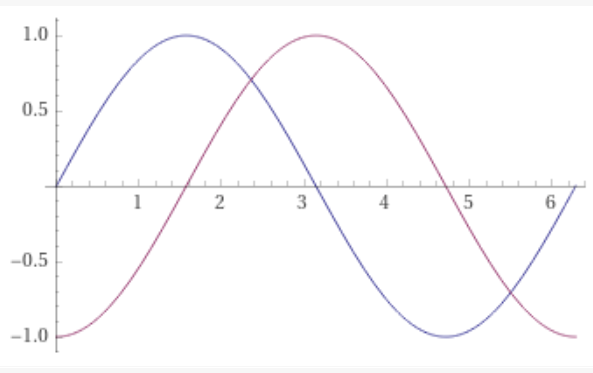
\includegraphics[width=0.9\textwidth]{05/phaseshift.png}};
\node at (-1.6,2.0) { \textcolor{blue}{not reflected}};
\node at (1.7,2.0)  { \textcolor{purple}{reflected}};
\end{TIKZP}
\begin{center}
{\small Thanks to Rick Roesler for this plot}
\end{center}
}
}{%
\Vskip{-4em}\begin{center}
\begin{TIKZP}[scale=2.0]
    \draw[thick,color=red] (0,0.5) -- ++(0.5,0);
    \visible<1,4->{\draw[->,thick,color=red] (0,0.5) -- ++(0.5,0) -- ++(0,-0.5);}
    \visible<1-3>{\draw[->,thick,color=red] (0.5,0.5) -- (1.0,0.5);}
    \visible<1-2,4->{\RotateAroundCenter{-45}{\BeamSplitter{}}}
\end{TIKZP}
\end{center}
\visible<5->{%
When reflected, we assume here that the photon experiences \textcolor<6->{purple}{a delay of $\frac{\pi}{2}$ radians} compared with \textcolor<6->{blue}{one passing through the beam splitter}.
}
}

\end{frame}

\begin{frame}{Analysis of the photon's paths}{A demonstration of interference}

\Vskip{-4em}\TwoUnequalColumns{0.55\textwidth}{0.45\textwidth}{%
\begin{itemize}
  \item<1-> A photon is measured \textcolor{NavyBlue}{here} using one of two paths:
  \begin{itemize}
      \item<2-> \textcolor{purple}{Here, the photon is reflected by a mirror, but passes through both beam splitters.  \alert<2>{There is no phase shift in this case.}}
      \item<3-> \textcolor{OliveGreen}{Here, the photon is reflected by each beam splitter.  \alert<3>{The accumulated delay is therefore $2\times \pi/2 = \pi$~radians.}}
  \end{itemize}
  \item<4-> \textcolor{NavyBlue}{Where the paths converge, the waves cancel, so there is no probability of measurement here.}
  \item<5> \textcolor{orange}{All photons are measured here.}
\end{itemize}
}{%
\Vskip{-2em}
\begin{center}
\begin{TIKZP}[scale=0.655]
\MZ{}
\draw[color=red] (1,0.5) -- (2.5,0.5);
\draw[color=purple] (2.5,0.5) -- ++(4,0) -- ++(0,-2);
\draw<2>[ultra thick,color=purple] (2.5,0.5) -- ++(4,0) -- ++(0,-3.5);
\draw[color=OliveGreen] (2.5,0.5) -- ++(0,-2) -- ++(4,0);
\draw<3>[ultra thick,color=OliveGreen] (2.5,0.5) -- ++(0,-2) -- ++(4,0) -- ++(0,-1.5);
\draw<1,5->[->,color=orange] (6.5,-1.5) -- ++(1.5,0);
\draw<1-4>[->,color=NavyBlue] (6.5,-1.5) -- ++(0,-1.5);
\end{TIKZP}
\MedSkip{}

\only<1-4>{
\begin{TIKZP}
\visible<2,4>{
\begin{scope}[color=purple]
\SineWave{1.0}
\end{scope}}
\visible<3,4>{
\begin{scope}[color=OliveGreen]
\SineWave{-1.0}
\end{scope}}
\end{TIKZP}}
\end{center}
\only<5->{
Physics experiments have confirmed this behavior.
We will soon look at how to model this behavior mathematically.}
}
\end{frame}

\begin{frame}{The quantum eraser}{This material can be skipped, but you may find it interesting.}
\begin{itemize}
    \item A \href{https://www.scientificamerican.com/article/slide-show-do-it-yourself-diy-quantum-eraser/}{do-it yourself} approach.
    \item This material from \href{https://www.physlab.org/wp-content/uploads/2016/07/machzehnder-v4.pdf}{here}
    \item PBS Space Time: \href{https://www.youtube.com/watch?v=8ORLN_KwAgs}{How the Quantum Eraser Rewrites the Past}
    \item PBS Space Time: \href{https://www.youtube.com/watch?v=2Uzytrooz44}{Quantum Eraser Lottery Challenge}
\end{itemize}
\end{frame}

\begin{frame}{Accounting for a phase shift of $\pi/2$ radians}{We use complex numbers.}
\Vskip{-3em}\TwoUnequalColumns{0.7\textwidth}{0.3\textwidth}{%
\begin{itemize}
    \item Recall the complex unit circle.  
    \item Suppose we begin with an amplitude $\alpha$, which already has an arbitrary phase shift.
    \item<2-> $\ExpPhase{0}\alpha = 1\times \alpha$ represents no (further) phase shift.
    \item<3-> The shift of $\alpha$ by $\theta$ radians is then $\ExpPhase{\theta}\alpha$.
   
    
\end{itemize}
}{%
\begin{center}
    \begin{TIKZP}
        \UnitComplexCircle{}
        \visible<4->{\TZPNorth{}
        \draw[->,ultra thick] (0,0) -- (0,1);}
        \visible<2->{\TZPEast{}}
        \visible<3>{\draw[->,thick] (1,0) arc (0:45:1) coordinate (z) ;
    \draw[thick] (0,0) -- (z) ;
    \draw (0.3,0) node[above right] {$\theta$};}
        \visible<4->{\TZPSouth{}
        \TZPWest{}}
    \end{TIKZP}
\end{center}
}
\OnlyRemark{4}{The shift of an amplitude by $\pi/2$ radians is effected through multiplication by $\ExpPhase{\pi/2} = i$.}
\end{frame}
\begin{frame}{Properties of phase shifts}{Complex math helps here too.}
\Vskip{-3em}\TwoUnequalColumns{0.7\textwidth}{0.3\textwidth}{%
\begin{itemize}
    \item<1-> A phase shift has no effect on the wave's magnitude:
    \[
    \Forall{\theta}{%
    \Mag{\ExpPhase{\theta}\alpha} = \Mag{\ExpPhase{\theta}} \times \Mag{\alpha} 
    = 1 \times \Mag{\alpha} = \Mag{\alpha}
    }
    \]
    \item<2-> A shift of $\alpha$ by $\theta$ radians followed
    by a shift of $\phi$ radians is given by
    \[
       \ExpPhase{\phi}\left(\ExpPhase{\theta}\alpha\right) = \ExpPhase{(\theta+\phi)}\alpha
    \]
    which walks counter-clockwise around the unit circle $\theta$ and then $\phi$ radians.
\end{itemize}
}{%
\begin{center}
    \begin{TIKZP}
        \UnitComplexCircle{}
        \TZPNorth{}\TZPSouth{}\TZPEast{}\TZPWest{}
        \visible<1->{
            \draw[->,thick] (1,0) arc (0:45:1) coordinate (z) ;
            \draw[thick] (0,0) -- (z) ;
            \draw (0.3,0) node[above right] {$\theta$};
        }
        \visible<2->{
            \draw[->,thick] (1,0) arc (0:135:1) coordinate (z) ;
            \draw[thick] (0,0) -- (z) ;
            \draw (0,0.2) node[above left] {$\phi$};
        }
    \end{TIKZP}
\end{center}
}
\end{frame}

\begin{frame}{Creating an equal superposition}{We can determine much about the amplitude from the desired probability.}
\Vskip{-3em}\TwoUnequalColumns{0.6\textwidth}{0.4\textwidth}{%
\begin{itemize}
    \item<1-> We begin with a ground state such as \ket{0}.
    \item<2-> From \ket{0}, we wish to create an equal superposition of \ket{0} and \ket{1}.
    \item<3-> That is, we want the probability of measuring either outcome to be $\frac{1}{2}$.
    \item<4-> From this we know the magnitude of the associated wave amplitudes must be $\frac{1}{\sqrt{2}}$.
    \item<5-> We are thus seeking the state
    \[ \alpha\ket{0} + \beta\ket{1} \]
    subject to $\Mag{\alpha} = \Mag{\beta} = \frac{1}{\sqrt{2}}$
\end{itemize}
}{%
\Vskip{-4em}\begin{center}
\begin{TIKZP}[scale=2.0]
    \draw[thick,color=red] (0,0.5) -- ++(0.5,0);
    \visible<1->{\draw[->,thick,color=red] (0,0.5) -- ++(0.5,0) -- ++(0,-0.5);}
    \visible<1->{\draw[->,thick,color=red] (0.5,0.5) -- (1.0,0.5);}
    \visible<1->{\RotateAroundCenter{-45}{\BeamSplitter{}}}
\end{TIKZP}
\end{center}
\visible<6->{
\BigSkip{}
Each wave amplitude must therefore be of the form
\[\frac{1}{\sqrt{2}}\ExpPhase{\theta} \]
}
}
\end{frame}
\def\BSG{%
\ensuremath{\frac{1}{\sqrt{2}}
\begin{pmatrix}
1 & i \\
i & 1
\end{pmatrix}}}

\section{Quantum gates}

\begin{frame}{Modeling the beam splitter}{Our first quantum gate}

\def\ralpha{\ensuremath{\textcolor{red}{\alpha}}}
\def\bbeta{\ensuremath{\textcolor{brown}{\beta}}}
\def\ralphap{\ensuremath{\textcolor{orange}{\alpha'}}}
\def\bbetap{\ensuremath{\textcolor{NavyBlue}{\beta'}}}


\Vskip{-3em}\TwoUnequalColumns{0.5\textwidth}{0.5\textwidth}{%
\visible<1->{Suppose the beam splitter is presented with a photon in superposition
    \[\ket{\psi}=
    \visible<1->{\ralpha\textcolor{red}{\ket{0}}}
    \visible<2->{+ \bbeta\textcolor{brown}{\ket{1}}
    = \SQB{\ralpha}{\bbeta}
    }
    \]}
    \visible<5->{%
    \Vskip{-1.5em}The output is then
    \begin{eqnarray*}
     \ket{\psi'} & = & \SQB{\ralphap{}}{\bbetap{}} \\
     \ralphap{} & = & \frac{1}{\sqrt{2}}\left(\visible<6->{\ralpha{}}
        + \visible<7->{i\bbeta{}}\right) \\
    \visible<8->{\bbetap{} & = & \frac{1}{\sqrt{2}}\left(\visible<9->{i\ralpha{}}
         + \visible<10->{\bbeta{}}\right)}
    \end{eqnarray*}}
}{%
\only<1-10>{%
\Vskip{-4em}
\begin{center}
\begin{TIKZP}[scale=2.5]
    \visible<1->{\RotateAroundCenter{-45}{\BeamSplitter{}}}
    \visible<1->{\draw[->,color=red] (0,0.5) node[left] {$\alpha$}  -- node[midway,below]  {\ket{0}} ++(0.5,0);}
    \visible<2->{\draw[->,color=brown] (0.5,1) node[above] {$\beta$} -- node[midway,right] {\ket{1}} ++(0, -0.5);}
    \visible<3->{\draw[->,color=orange] (0.5,0.5) -- (1.0,0.5) node[right] {$\alpha'$};}
    \visible<4->{\draw[->,color=NavyBlue] (0.5,0.5) -- ++(0,-0.5) node[below] {$\beta'$};}
    
\end{TIKZP}
\end{center}
\only<3-4>{We want to compute the effect of the beam splitter in creating a superposition of outputs: \textcolor{orange}{photon traveling east} and \visible<4->{\textcolor{NavyBlue}{photon traveling south}}}
\only<5-7>{\ralphap{} is composed of an equal fraction of \only<6-7>{\ralpha{} continuing right} \only<7>{and \bbeta{} reflecting to the right with a $\frac{\pi}{2}$ phase shift.}}
\only<8-10>{\bbetap{} is composed of an equal fraction of \only<9-10>{\ralpha{} reflecting down with a $\frac{\pi}{2}$ phase shift} \only<10>{and \bbeta{} continuing down.}}
}%
\only<11->{%
We can model the effect of the beam splitter using the following matrix algebra:
\[
\SQB{\ralphap{}}{\bbetap{}} = 
\BSG{} \SQB{\ralpha}{\bbeta}
\]
and we view the beam splitter as represented mathematically as
\[
\BSG{}
\]
}
}
\end{frame}

\begin{frame}{Applying the beam splitter to our example}{Matrix multiplication models the cumulative effect of gates.}

\TwoUnequalColumns{0.6\textwidth}{0.4\textwidth}{%
\Vskip{-2em}\begin{itemize}
    \only<1-2>{
    \item We begin with the photon in state \SQB{1}{0}.}
    \only<2-3>{\item At the first beam splitter, we obtain the state
    \[ \BSG{} \SQB{1}{0} = \frac{1}{\sqrt{2}} \SQB{1}{i}
    \]}
    \only<3-4>{\item The mirrors flip the sense of two paths with respect to the second beam splitter.  We therefore apply a gate to swap the two components and obtain
    \[
    \XMatrix{} \RootTwo{}\SQB{1}{i} = \RootTwo{}\SQB{i}{1}
    \]}
    \only<4-5>{\item The final beam splitter produces
    \[
    \BSG{}\RootTwo{}\SQB{i}{1} = \frac{1}{2}\SQB{2i}{i^{2}+1} = \SQB{i}{0}
    \]}
    \only<5>{\item The interference canceled the bottom component.    
    \alert{This explains why the bottom device never measures any photons in this setup.}
    \item
    We can also see the top component is rotated by $\pi/2$ radians.  The superpositions measured \textcolor{orange}{by this device} each experienced one beam-splitter reflection.}
\end{itemize}
}{%
\begin{center}
    \Vskip{-3em}\begin{TIKZP}[scale=0.5]
        \MZ{}
        \visible<2>{\Shift{2}{0}{\RotateAroundCenter{-45}{\BeamSplitter[ultra thick]{}}}}
        \visible<4>{\Shift{6}{-2}{\RotateAroundCenter{-45}{\BeamSplitter[ultra thick]{}}}}
        \draw[color=red] (1,0.5) -- (2.5,0.5);
        \draw<1>[ultra thick,color=red] (1,0.5) -- (2.5,0.5);
        \draw[color=purple] (2.5,0.5) -- ++(4,0) -- ++(0,-2);
        \draw[color=OliveGreen] (2.5,0.5) -- ++(0,-2) -- ++(4,0);
        \draw[->,color=orange] (6.5,-1.5) -- ++(1.5,0);
        \draw[->,color=NavyBlue] (6.5,-1.5) -- ++(0,-1.5);
    \end{TIKZP}
    \begin{TIKZP}[scale=1.5]
    \visible<1->{\RotateAroundCenter{-45}{\BeamSplitter{}}}
    \visible<1->{\draw[->,color=red] (0,0.5) node[left] {$\alpha$}  -- node[midway,below]  {\ket{0}} ++(0.5,0);}
    \visible<1->{\draw[->,color=brown] (0.5,1) node[above] {$\beta$} -- node[midway,right] {\ket{1}} ++(0, -0.5);}
    \visible<1->{\draw[->,color=orange] (0.5,0.5) -- (1.0,0.5) node[right] {$\alpha'$};}
    \visible<1->{\draw[->,color=NavyBlue] (0.5,0.5) -- ++(0,-0.5) node[below] {$\beta'$};}
    
\end{TIKZP}
\end{center}
}
    
\end{frame}

\begin{frame}{Quantum gates as matrices}{What properties must they have?}

\begin{itemize}
    \item Recall that the quantum state of a single qubit can be represented by the ket
    $\SQB{\alpha}{\beta}$, where $\alpha$ and $\beta$ are complex numbers.  We require $\Prob{\alpha}+\Prob{\beta}=1$.  Such vectors are called \href{https://en.wikipedia.org/wiki/Unit_vector}{unit vectors}.
    \item A matrix can represent the action of a quantum gate, but it must have the following properties:
    \begin{itemize}
        \item It must be \href{https://en.wikipedia.org/wiki/Reversible_computing}{reversible}. We have already studied this property.
        \item It must be \emph{length-preserving}.  If $U$ is such a matrix, then $\Implies{\Mag{\alpha}=1}{\Mag{U\alpha}=1}$. Informally, no \Quote{probability} is gained or lost by application of $U$.
    \end{itemize}
     
\end{itemize}
    The matrices we seek are \href{https://en.wikipedia.org/wiki/Unitary_matrix}{unitary}.   We next investigate their definition and properties.
\end{frame}

\begin{frame}{Unitary matrix}{Definition and properties \LinkArrow{https://en.wikipedia.org/wiki/Unitary_matrix}}

\Definition{%
The matrix $U$ is \emph{unitary} iff $U\Conj{U}=\Conj{U}U=\Identity$}
\begin{center}Equivalent conditions\end{center}

\TwoColumns{%

\begin{itemize}
    \item $U$ is unitary
    \item \Conj{U} is unitary
    \item $U$ is invertible with $\Inverse{U}=\Conj{U}$
    \item The columns of $U$ form an \href{https://en.wikipedia.org/wiki/Orthonormal_basis}{orthonormal basis}; so do the rows.
\end{itemize}
}{%
\begin{itemize}
    \item $U$ is a \href{https://en.wikipedia.org/wiki/Normal_matrix}{normal matrix} whose eigenvalues lie on the (real) unit circle.
\end{itemize}
}

\end{frame}

\section{Summary}
\begin{frame}{Summary}{What have we learned?}
\begin{itemize}
    \item A quantum state is represented by a column vector called a \emph{ket}.  The \href{https://en.wikipedia.org/wiki/Qubit\#Standard_representation}{standard computational basis} for a single qubit uses $\ket{0}=\PZero{}$ and $\ket{1}=\POne{}$.
    \item Superpositions are expressed as linear combinations of basis states.  
    \item The wave amplitude on each basis state is a complex number, which expresses both magnitude and phase.
    \item We model a quantum gate using a unitary matrix.  For a single qubit, such matrices are $2\times 2$.
    \item The effect of a gate on a quantum state is computed using matrix multiplication.
\end{itemize}
    
\end{frame}
\frame{Assignment ps1}
\frame{Programming assignment q0}

\SetTitle{6}{A single qubit}{Representation and some quantum gates}{06}

\section{Overview}
\begin{frame}{Overview}{What we will cover}
\begin{itemize}
    \item We develop an efficient representation for a single quantum bit (qubit), parameterized by two real values.
    \item We introduce the Bloch sphere: a compelling visualization of a single qubit.
    \item We introduce the Hadamard gate that transforms \ket{0} into a uniform superposition of \ket{0} and \ket{1}.
    \item We introduce the \emph{Pauli} gates and their associated unitary matrices.
    \item We develop a general approach to rotating a qubit around each axis of the Bloch sphere.
\end{itemize}
\end{frame}

\section{Efficient characterization}

\begin{frame}{State space}{Definition}
\Vskip{-3em}\Postulate{State Space}{The state of a quantum system is a unit vector in a complex \href{https://en.wikipedia.org/wiki/Hilbert_space}{Hilbert space}}
\begin{itemize}
    \item We need a Hilbert space, rather than the simpler \href{https://en.wikipedia.org/wiki/Euclidean_space}{Euclidean space}, because we use complex values to represent state.
    \item We have used two dimensions to specify a single qubit, one each for $\alpha$ and $\beta$: $\ket{\psi}=\SQB{\alpha}{\beta}$, where
    $\Prob{\alpha}+\Prob{\beta}=1$.
  
    \item The state of an $n$-qubit system is a unit column vector (ket)  of $\TwoToThe{n}$ complex values.
\end{itemize}
\OnlyRemark{1}{%
We next examine a more concise and visually compelling definition of a qubit.
}
\end{frame}

\begin{frame}{Coordinates for a qubit}{Cartesian and polar}
\Vskip{-5em}\TwoUnequalColumns{0.4\textwidth}{0.6\textwidth}{%
\ColHead{Cartesian}
\begin{itemize}
    \item $\ket{\psi}=\alpha\ket{0} + \beta\ket{1}$ with $\Mag{\alpha}^2+\Mag{\beta}^2=1$.
    \item Letting
    \begin{itemize}
        \item $\alpha=\Complex{a_{0}}{b_{0}}$
        \item $\beta=\Complex{a_{1}}{b_{1}}$
    \end{itemize}
    \item This requires \alert{four real parameters}
\end{itemize}
}{%
\ColHead{Polar}
\begin{itemize}
    \item Write $\alpha = r_{a}\left(\cos\theta_{a}+\NiceI \sin\theta_{a}\right) = \Polar{r_{a}}{\theta_{a}}$
    \item Write $\beta = r_{b}\left(\cos\theta_{b}+\NiceI \sin\theta_{b}\right) = \Polar{r_{b}}{\theta_{b}}$
    \item Then \begin{eqnarray*} \ket{\psi} & = & \Polar{r_{a}}{\theta_{a}}\ket{0} + \Polar{r_{b}}{\theta_{b}}\ket{1} \\
    & = & \visible<1>{\ExpPhase{\theta_{a}}}\left( \alert<4>{r_{a}}\ket{0} + \Polar{\alert<4>{r_{b}}}{
    \only<1-2>{(\theta_{b}-\theta_{a})}
    \only<3->{\alert<4>{\phi}}
    }\ket{1} \right)
    \end{eqnarray*}
    \item<2-> Discard $\ExpPhase{\theta_{a}}$ as a global phase
    \item<3-> Let $\phi=\theta_{b}-\theta_{a}$
    \item<4-> So we need just \alert{three real parameters}
\end{itemize}
}
\end{frame}

\def\Bloch#1#2{%
\ensuremath{%
\cos{\frac{\textcolor{\RCtwo}{#1}}{2}}\ket{0} + \Polar{}{\textcolor{\RCone}{#2}}\sin{\frac{\textcolor{\RCtwo}{#1}}{2}}\ket{1}}}

\section{Bloch sphere}

\begin{frame}{Can we do better?}{Yes!  It takes only two real parameters to denote the state of one qubit}
\begin{itemize}
   \item We start with three real parameters:
   \( \ket{\psi}= r_{a}\left( \ket{0} + r_{b}\ExpPhase{\phi}\ket{1}\right) \)
   \item We have not yet accounted for the unit nature of \ket{\psi}.   
   \item We require $r_{a}^{2}+r_{b}^{2}=1$ which implies \And{r_{a}^{2} \leq 1}{r_{b}^{2} \leq 1}. 
   \item We can show $\Implies{x^{2}\leq 1}{-1 \leq x \leq 1}$.
   \item<2-> We therefore substitute for $r_{a}$ and $r_{b}$ as follows:
   \[
     r_{a} = \cos{\frac{\theta}{2}}, 
     r_{b} = \sin{\frac{\theta}{2}} \]
   The use of $\theta/2$ is arbitrary for now but will work out well later.
   \item<3-> We can thus characterize $\ket{\psi}$ using only \alert{two (angular) real parameters}:
   \[ \ket{\psi} = \Bloch{\theta}{\phi}
   \]
\end{itemize}

    
\end{frame}

\begin{frame}{From polarizing filters to a sphere}{The angular separation between the basis states changes}
\Vskip{-3em}\TwoColumns{%
\begin{itemize}
    \item<1-> With polarizing filters, our bases were horiziontal \visible<2->{and vertical, so they were separated by \Degrees{90}.}
    \item<3-> We imposed a \Degrees{90} angular separation between these bases logically as well.
    \item<4-> We are about to use a \emph{sphere} to capture quantum state.  To use the entire sphere, we locate \ket{0} at the north pole and \ket{1} at the south pole.
    \item<5-> In that depiction, the basis states are separated by \Degrees{180}.
\end{itemize}
}{%
\Vskip{-3em}\begin{center}
\begin{TIKZP}
\visible<3->{
\draw[->,ultra thick] (0,0) -- (1,0) node[right] {\ \ket{0}};
\draw[->,ultra thick] (0,0) -- (0,1) node[above] {\ket{1}};
}
\visible<1->{\begin{scope}[draw=\RCtwo,rotate=90]\PFilter{-1}{-1.2}{1}{1.2}{20}\end{scope}}
\visible<2->{\begin{scope}[draw=\RCthree]\PFilter{-1}{-1.2}{1}{1.2}{20}\end{scope}}
\end{TIKZP}
\end{center}
\visible<4->{%
\begin{center}
    \begin{BlochSphere}[scale=1]{60}{115}
    \BlochSpherePhiTheta{}
     \TZPoint{0,0,1}{\ket{0}}{right}
     \TZPoint{0,0,-1}{\ket{1}}{below}
    \end{BlochSphere}
\end{center}}
}
\end{frame}

\begin{frame}{Our two-parameter characterization}{It meshes well with our studies so far}
\[ \Bloch{\theta}{\phi} \]
\begin{itemize}
    \item The parameter \textcolor{\RCtwo}{$\theta$} trades wave amplitude between \ket{0} and \ket{1}.
    \item Only the relative phase between \ket{0} and \ket{1} matters for interactions.  
    \item This formulation ascribes the phase difference to \ket{1}, using a walk of \textcolor{\RCone}{$\phi$} radians counterclockwise around the complex unit circle, starting at 0~radians.
    \item This formulation of state makes clear that while only two real-valued parameters are needed, the number of states is \href{https://en.wikipedia.org/wiki/Uncountable_set}{uncountably infinite}.
    
\end{itemize}
    
\end{frame}

\begin{frame}{Recall the beam splitter}{We characterize two of its states using our new formula}
\[ \Bloch{\theta}{\phi} \]
    \begin{itemize}
        \item The state of the photon was initially $\Bloch{0}{0} = \SQB{1}{0}$
        \item After one beam splitter we obtained \[ \Bloch{\pi/2}{\pi/2} = \frac{1}{\sqrt{2}} \SQB{1}{i} \]
    \end{itemize} 
\end{frame}

\begin{frame}{The Bloch sphere}{Our two angular parameters determine a point on the unit sphere}
\TwoColumns{%
\[ \ket{\psi} = \Bloch{\theta}{\phi} \]
\begin{itemize}

\item \ket{\psi} is located 
\begin{itemize}
    \item  \textcolor{\RCone}{$\phi$} radians off the $x$~axis and 
    \item \textcolor{\RCtwo}{$\theta$} radians off the $z$~axis.
\end{itemize}
\item We locate states \emph{on} the unit sphere, but the distance from the center of the sphere has no meaning here.  

A more general interpretation of the sphere ascribes meaning to interior points.
\end{itemize}
}{%
\Vskip{-3em}\begin{BlochSphere}[scale=2.5]{60}{115}
    
    \BlochSpherePhiTheta{}
    \TZPoint{theta}{\ket{\psi}}{above right}
\end{BlochSphere}
}
\end{frame}

\begin{frame}{Correspondence between the formula and the sphere}{We see why the formula cuts the angle in half}
\TwoUnequalColumns{0.5\textwidth}{0.5\textwidth}{%
\begin{itemize}
  \item<2-> We locate \ket{0} at \PhiTheta{0}{0} using \Bloch{0}{0}.  The choice of \textcolor{\RCone}{$\phi$} doesn't matter when $\textcolor{\RCtwo}{\theta}=0$.
  \item<3-> We locate \ket{1} at $\PhiTheta{0}{\pi}$ using $\Bloch{\pi}{0}$.
  \item<4-> From the picture, \textcolor{\RCone}{$\phi$} doesn't matter when $\textcolor{\RCtwo}{\theta}=\pi$.  How can this be?
\end{itemize}
}{%
\only<1-4>{%
\[ \ket{\psi} = \Bloch{\theta}{\phi} \]}
\only<5>{%
\[ \ket{\psi} =  \ExpPhase{\textcolor{\RCone}{\phi}} \ket{1} \]
}%
\only<1-4>{%
\begin{BlochSphere}[scale=1.5]{60}{115}
    
    \BlochSpherePhiTheta{}
    \visible<2->{\TZPoint{0,0,1}{$\ket{0}$}{right}}
    \visible<3->{\TZPoint{0,0,-1}{$\ket{1}$}{right}}
    
\end{BlochSphere}}%
\only<5>{%
\begin{itemize}
\item With $0$ as the amplitude on \ket{0}, any phase on \ket{1} with $\textcolor{\RCone}{\phi}\not=0$ can be canceled with an appropriate global phase of 
  \ExpPhase{(-\textcolor{\RCone}{\phi})} on \ket{\psi}.
\item Global phases can be ignored as they do not affect measurements or interactions.
\end{itemize}
}
}
\end{frame}

\begin{frame}{The computational basis}{Measurement outcomes are related to proximity to the north or south pole}
\TwoUnequalColumns{0.6\textwidth}{0.4\textwidth}{%
\begin{itemize}
  \item<1-> The north and south poles, \ket{0} and \ket{1}, respectively, are our \emph{standard} or \emph{computational basis}.
   All other points on the sphere are superpositions of that basis.
   \item<2-> The probability of measuring \ket{0} or \ket{1} is related to how close the state is to the north or south pole, respectively, which is represented by $\textcolor{\RCtwo}{\theta}$.
   \item<3-> The probability of measuring \ket{0} is $\cos^{2}(\textcolor{\RCtwo}{\theta}/2)$.  At the equator, we are equally likely to measure \ket{0} or \ket{1}.
\end{itemize}
}{%
\[ \ket{\psi} = \Bloch{\theta}{\phi} \]
\begin{BlochSphere}[scale=1.5]{60}{115}
    
    \BlochSpherePhiTheta{}
    \visible<2->{\TZPoint{0,0,1}{$\ket{0}$}{right}}
    \visible<3->{\TZPoint{0,0,-1}{$\ket{1}$}{right}}
    
\end{BlochSphere}
}
\end{frame}

{%
\def\Sket#1{%
\ket{\hbox to 4ex{\hfil\ensuremath{#1}\hfil}}}%
\def\R#1{\mbox{\textcolor{\RCone}{#1}}}%
\def\B#1{\mbox{\textcolor{\RCtwo}{#1}}}%
\begin{frame}{Navigating the Bloch sphere}{Other points of interest}


\Vskip{-4em}\TwoUnequalColumns{0.6\textwidth}{0.4\textwidth}{%
\begin{center}
    \begin{tabular}{ccc}
        State & \textcolor{\RCone}{$\phi$} & \textcolor{\RCtwo}{$\theta$} \\
        \visible<1->{\Sket{0} & \R{$0$} & \B{$0$} \\}%
        \visible<1->{\Sket{1} & \R{$0$} & \B{$\pi$} \\}%
        \visible<2->{\Sket{+x} & \R{$0$} & \B{$\pi/2$} \\}%
        \visible<3->{\Sket{-x} & \R{$0$} & \B{$-\pi/2$} \\}%
        \only<3-4>{\Sket{-x} & \R{$\pi$} & \B{$\pi/2$} \\}%
        \visible<5->{\Sket{+y} & \R{$\pi/2$} & \B{$\pi/2$} \\}%
        \visible<6->{\Sket{-y} & \R{$-\pi/2$} & \B{$\pi/2$} \\}%
    \end{tabular}
\end{center}
\only<4>{\Vskip{-5em}States \ket{+x} and \ket{-x} are also called \ket{+} and \ket{-}, respectively.  They are more familiar as:
\begin{eqnarray*} \ket{+} & = & \frac{1}{\sqrt{2}} \SQB{1}{1} \\
\ket{-} & = & \frac{1}{\sqrt{2}} \SQB{1}{-1}
\end{eqnarray*}
}%

}{%
\[ \ket{\psi} = \Bloch{\theta}{\phi} \]
\begin{BlochSphere}[scale=1.5]{60}{115}
    
    \BlochSpherePhiTheta{}
    \visible<1>{\TZPoint{0,0,1}{$\ket{0}$}{right}}
    \visible<1>{\TZPoint{0,0,-1}{$\ket{1}$}{right}}
    \visible<2-3>{\TZPoint{1,0,0}{$\ket{+x}$}{right}}
    \visible<3>{\TZPoint{-1,0,0}{$\ket{-x}$}{right}}
    \visible<5-6>{\TZPoint{0,1,0}{$\ket{+y}$}{above}}
    \visible<6>{\TZPoint{0,-1,0}{$\ket{-y}$}{right}}
\end{BlochSphere}
}
\Exercise{y}{What are +y and -y, expressed in the standard basis?}
\end{frame}
}

\begin{frame}{Switching between bases}{We consider here the standard and Hadamard bases}
\TwoUnequalColumns{0.7\textwidth}{0.3\textwidth}{%
\begin{itemize}
    \item Typically, our computations begin and end (with measurements) in the standard basis.
    \item We often create a uniform superposition of the standard basis states, \ket{+} or \ket{-}, which together form the \href{https://en.wikipedia.org/wiki/Quantum_logic_gate\#Hadamard_gate}{Hadamard} basis in quantum computing.
    \item<1-> How?  We need a transformation (unitary matrix) \Hadamard{} that sends $\ket{0}\mapsto \ket{+}$ and $\ket{1}\mapsto \ket{-}$.
    \item<3-> From linear algebra, the columns of \Hadamard{} are the transformed versions of \textcolor<4->{\RCtwo}{\ket{0}} and \textcolor<5->{\RCthree}{\ket{1}}.
    \item<6-> Because it is symmetric and its entries are real, \mbox{\Hadamard{} = \Conj{\Hadamard{}}}  $\rightarrow$ \Hadamard{} is also its own inverse.
    
\end{itemize}
}{%
\visible<2->{%
\begin{eqnarray*}
    \SQB{1}{0} & \mapsto & \textcolor<3->{\RCtwo}{\frac{1}{\sqrt{2}}\SQB{1}{1}} \\
    \SQB{0}{1} & \mapsto & \textcolor<3->{\RCthree}{\frac{1}{\sqrt{2}}\SQB{1}{-1}}
    \end{eqnarray*}}
\visible<4->{%
\[
\Hadamard{} = \HMatrix{}
\]
\begin{TIKZP}[overlay]
  \draw[white] (0,0) circle(1pt);  % anchor
  \draw<4-5>[\RCtwo,thick] (2.25,0.7) ellipse(0.3 and 0.6);
  \draw<5>[\RCthree,thick] (3, 0.7) ellipse (0.3 and 0.6);
\end{TIKZP}
}
}
\end{frame}

\begin{frame}{Physics and the Bloch sphere}{Models electron spin in space}
\Vskip{-4em}\TwoUnequalColumns{0.8\textwidth}{0.2\textwidth}{%
\begin{itemize}
\item The labeled axes on the Bloch sphere are often used in physics to model spin in each of the three physical dimensions:
\begin{description}
\item[z axis] spin up or down
\item[x axis] spin in or out
\item[y axis] spin left or right
\end{description}
\item In quantum computing we almost always use the standard basis of \ket{0} and \ket{1} (the z axis).
\item The named axes are mutually orthogonal. \Exercise{Orthogonal Axes}{Prove orthogonality of the x, y, and z axes}
\item While we can characterize two of the dimensions using only real values (the z--x plane, where $\textcolor{\RCone}{\phi}=0$), we require complex values to admit a third mutually orthogonal dimension (y).

\end{itemize}
}{%
\begin{center}
    \begin{BlochSphere}[scale=1]{60}{115}
    
    \BlochSpherePhiTheta{}
    \end{BlochSphere}
\end{center}
}

\end{frame}

\begin{frame}{What other bases are there?}{Quite a few}
\Definition{Two points on the Bloch sphere are \emph{antipodal} if they determine a line that passes through the center of the sphere.}
\TwoColumns{%
\begin{itemize}
    \item Every pair of antipodal points determines an orthogonal basis for the quantum state of a single qubit. \Exercise{Antipodal points determine a basis}{Prove that antipodal points on the Bloch sphere are orthogonal.}
    \item Using linear algebra, we can express any state \ket{\psi} in any basis. \LinkArrow{https://www.youtube.com/watch?v=P2LTAUO1TdA}
\end{itemize}
}{%
\begin{center}
\begin{BlochSphere}[scale=1.5]{60}{115}
    \BlochSpherePhiTheta{}
\end{BlochSphere}
\end{center}
}
\end{frame}

%% \begin{frame}{Antipodal points are orthogonal}{Leave as exercise?}
%% \ToDo{include or not?}
%% \end{frame}

\section{The Pauli matrices}

\begin{frame}{Overview of the Pauli matrices}{We use these as gates in quantum computation}

\begin{itemize}
    \item There are three \href{https://en.wikipedia.org/wiki/Pauli_matrices}{Pauli matrices} that are named for the three axes of the Bloch sphere.
    \item Each matrix has the property of rotating a state by $\pi$ radians about its associated axis.
    \item Each gate is its own inverse.
    \item We will develop a universality argument:  any quantum gate can be realized using a linear combination of the Pauli matrices.
    \item The gates we study here are quantum gates, used in the middle of a quantum circuit.  We can also think of these gates as \emph{measurement operators} but we study that later.
\end{itemize}
    
\end{frame}

\begin{frame}{Pauli \PauliZ{}}{A gate that changes the sign of \ket{1}}

\TwoUnequalColumns{0.6\textwidth}{0.4\textwidth}{%
\[
\PauliZ{} = \ZMatrix{}
\]
\begin{itemize}
    \item<1-> This matrix transforms a state as follows: \[ \ApplyGate{\PauliZ}{\SQB{\alpha}{\beta}} =  \SQB{\alpha}{-\beta} \]
    \item<2-> However, two states are unaffected by \PauliZ{}:
    \begin{itemize}
       \item $\ApplyGate{\PauliZ}{\left(\ket{0}=\SQB{1}{0}\right)} = \ket{0}$
       \item $\ApplyGate{\PauliZ}{\left(\ket{1}=\SQB{0}{1}\right)} = -\ket{1}\equiv \ket{1}$
    \end{itemize}
\end{itemize}
}{%
\Vskip{-4em}\begin{center}
    \begin{BlochSphere}[scale=1]{60}{115}
    \BlochSpherePhiTheta{}
     \TZPoint{0,0,1}{\ket{0}}{right}
     \TZPoint{0,0,-1}{\ket{1}}{below}
    \end{BlochSphere}
\end{center}
\only<2>{%
\Vskip{-2.5em}Such states are called eigenstates (or \href{https://en.wikipedia.org/wiki/Eigenvalues_and_eigenvectors}{eigenvectors}) of \PauliZ{}.  A matrix transforms an eigenstate into a multiple $\lambda$ of itself;  $\lambda$ is called an eigenvalue of the matrix.  Here, $\PauliZ{}\ket{0} = +1\ket{0}$ and $\PauliZ{}\ket{1}=-1\ket{1}$.
}
\only<3>{%
\Vskip{-2em}\PauliZ{} affects all other states, off the z axis, for example
\begin{eqnarray*}
\ApplyGate{\PauliZ}{\ket{+}} & = & \ket{-} \\
\ApplyGate{\PauliZ}{\ket{-}}  & = & \ket{+}
\end{eqnarray*}
rotations of $\pi$ radians around the z~axis.
}}
\end{frame}

\begin{frame}{Pauli \PauliX{}}{Also called the \NamedGate{NOT} gate}

\TwoUnequalColumns{0.6\textwidth}{0.4\textwidth}{%
\[
\PauliX{} = \XMatrix{}
\]
\begin{itemize}
    \item<1-> This transformation exchanges the amplitudes: \[ \ApplyGate{\PauliX}{\SQB{\alpha}{\beta}} =  \SQB{\beta}{\alpha} \]
    \item<2-> The two eigenstates are \ket{+x} and \ket{-x}. \Exercise{unaffected points}{Show that X doesn't affect +x or -x.}
    \item<3-> This gate maps $\ket{0}\mapsto\ket{1}$ and \VV{}.
\end{itemize}
}{%
\begin{center}
    \begin{BlochSphere}[scale=1]{60}{115}
    \BlochSpherePhiTheta{}
    \TZPoint{1,0,0}{\ket{x}}{left}
    \TZPoint{-1,0,0}{\ket{-x}}{right}
    \end{BlochSphere}
\end{center}
\PauliX{} generally
rotates a state  by $\pi$ radians around the x~axis.
}
\end{frame}

\begin{frame}{Pauli \PauliY{}}{Exchanges amplitudes and imposes a sign change}

\TwoUnequalColumns{0.6\textwidth}{0.4\textwidth}{%
\[
\PauliY{} = \YMatrix{}
\]
\begin{itemize}
    \item<1-> This transformation exchanges the amplitudes and imposes a relative sign change: \[ \ApplyGate{\PauliY}{\SQB{\alpha}{\beta}} =  \SQB{-\NiceI\beta}{i\alpha} = -\NiceI\SQB{\beta}{-\alpha} \equiv \SQB{\beta}{-\alpha} \]
    \item<2-> The two eigenstates are \ket{+y} and \ket{-y}. \Exercise{unaffected points}{Define +y and -y in the standard basis and show that Paul Y doesn't affect +y or -y.}
    \item<3-> This gate maps $\ket{0}\mapsto\ket{1}$ and \VV{}.
\end{itemize}
}{%
\begin{center}
    \begin{BlochSphere}[scale=1]{60}{115}
    \BlochSpherePhiTheta{}
    \TZPoint{0,1,0}{\ket{y}}{above}
    \TZPoint{0,-1,0}{\ket{-y}}{left}
    \end{BlochSphere}
\end{center}
\PauliY{} generally
rotates a state  by $\pi$ radians around the y~axis.  
\visible<3>{\MedSkip{}This gate also maps $\ket{+} \mapsto \ket{-}$ and \VV{}.}
}
\end{frame}

\begin{frame}{Properties of Pauli gates}{These should be apparent from our study so far}
\begin{center}
$\PauliX{}=\XMatrix{}$
$\PauliY{}=\YMatrix{}$
$\PauliZ{}=\ZMatrix{}$
\end{center}
\begin{itemize}
    \item Each matrix is \href{https://en.wikipedia.org/wiki/Involutory_matrix}{involutory} (each is its own inverse).
    \item These relations can be verified by computing the appropriate products:
    \begin{center}
    { \setlength{\tabcolsep}{3pt}%
    \begin{tabular}{rcrl@{\hspace{3em}}rcrl@{\hspace{3em}}rcrl} \setlength{\tabcolsep}{1pt}
        \PauliX{}\PauliY{} & = & \NiceI &\PauliZ{} & \PauliZ{}\PauliX{} & = & \NiceI &\PauliY{} & \PauliY{}\PauliZ{} & = & \NiceI &\PauliX{} \\
        \PauliY{}\PauliX{} & = & $-\NiceI$ &\PauliZ{} &  \PauliX{}\PauliZ{} & = & $-\NiceI$ &\PauliY{} & \PauliZ{}\PauliY{} & = & $-\NiceI$ &\PauliX{}
    \end{tabular}}
    \end{center}
    \item Each matrix has \href{https://en.wikipedia.org/wiki/Eigenvalues_and_eigenvectors}{eigenvalues} $\pm 1$.
    \item Each Pauli matrix rotates all states by $\pi$ radians about its associated axis, except the two states at the intercept of its axis with the unit Bloch sphere.  The eigenstates are therefore those intercepts.
\end{itemize}
\end{frame}

%%
%% This material might move to module 12
%%
\begin{frame}{Eigenvalues of the Pauli gates}{And their corresponding eigenvectors}
\only<1-5>{%
\begin{itemize}
    \item<1-> In quantum computing, a \href{https://en.wikipedia.org/wiki/Measurement_in_quantum_mechanics}{measurement of a quantum system} is modeled by an operator $M$ called an \href{https://en.wikipedia.org/wiki/Observable}{observable}.  We can generally view the measurement as yielding $+1$ or $-1$.
    \item<2-> After observation, the system is in a state $\psi$ such that subsequent applications of $\psi$ certainly yield the same measurement.
    \item<3-> If a system has been measured by an operator $M$ and it entered some state $\psi$, then we must have \[ M\psi = \lambda\psi \] where $\lambda=\pm 1$ is the measured result.
    \item<4-> The above equation is the \href{https://en.wikipedia.org/wiki/Eigenvalues_and_eigenvectors\#Formal_definition}{definition} of an eigenvalue~$\lambda$ and its eigenvector~$\psi$.
    \item<5-> For qubits, measurement operators yield $\pm 1$ and there will be a distinct eigenvector for each of those eigenvalues.
\end{itemize}}%
\only<6->{%
\TwoColumns{%
\only<6-12>{%
\begin{itemize}
    \item<6-> Each Pauli matrix is an observable.
    \item<7-> The \PauliZ{} matrix corresponds to the \href{https://en.wikipedia.org/wiki/Qubit\#Standard_representation}{computational basis}, because its eigenvectors are \visible<8->{\alert<8>{\ket{0}}} \visible<9->{and \alert<9>{\ket{1}}.}
    \item<10-> When an \alert<10>{arbitrary state~$\psi$}\visible<11->{ is measured as \ket{0} or \ket{1}, subsequent applications of \PauliZ{} produce the same eigenvalue and eigenvector.}  
    \item<12-> If $\psi$ happens to be \ket{0} or \ket{1}, then re-measurement must yield same state.
\end{itemize}}%
\only<13->{%
\begin{itemize}
    \item<13-> Consider the observable \PauliX{} with eigenvectors \visible<14->{\alert<14>{\ket{+}}} \visible<15->{and \alert<15>{\ket{-}}.}
\end{itemize}
}
}{%
\only<8-12>{%
\begin{alignat*}{5}
    \ZMatrix{} & \alert<8>{\PZero{}} & \mbox{ = } & +1  & \alert<8>{\PZero{}}  \\
    \visible<9->{\ZMatrix{} & \alert<9>{\POne{}} & \mbox{ = } & -1  & \alert<9>{\POne{}} }
\end{alignat*}}%
\only<13->{%
\begin{alignat*}{5}
    \XMatrix{} & \alert<14>{\PHad{}} & \mbox{ = } & +1  & \alert<14>{\PHad{}}  \\
    \visible<15->{\XMatrix{} & \alert<15>{\PHadm{}} & \mbox{ = } & -1  & \alert<15>{\PHadm{}} }
\end{alignat*}}
\begin{center}
\begin{TIKZP}
\visible<8->{
\draw[->,ultra thick] (0,0) -- (1,0) node[right] {\ \alert<8>{\ket{0}}};
\draw[->,ultra thick] (0,0) -- (0,1) node[above] {\alert<9>{\ket{1}}};
\visible<10>{\alert{\draw[->,thick] (0,0) -- (30:1) node[above] {$\psi$};}}
\visible<14>{\alert{\draw[->,thick] (0,0) -- (45:1) node[above] {\ket{+}};}}
\visible<15>{\alert{\draw[->,thick] (0,0) -- (-45:1) node[right] {\ket{-}};}}
}
\visible<8>{\begin{scope}[draw=\RCtwo,rotate=90]\PFilter{-1}{-1.2}{1}{1.2}{20}\end{scope}}
\visible<9>{\begin{scope}[draw=\RCthree]\PFilter{-1}{-1.2}{1}{1.2}{20}\end{scope}}
\visible<14>{\begin{scope}[draw=\RCtwo,scale=0.7,rotate=-45]\PFilter{-1}{-1.2}{1}{1.2}{20}\end{scope}}
\visible<15>{\begin{scope}[draw=\RCthree,scale=0.7,rotate=45]\PFilter{-1}{-1.2}{1}{1.2}{20}\end{scope}}
\end{TIKZP}
\end{center}
}
}

\end{frame}
%%
%% End of stuff that might move to module 12
%%
{%
\def\Redify#1{\textcolor{RedOrange}{#1}}%
\def\Bluify#1{\textcolor{\RCtwo}{#1}}%
\def\Term#1{\frac{i^{#1}\theta^{#1}A^{#1}}{#1!}}%
\def\TermA#1{\frac{i\theta^{#1}A}{#1!}}%
\def\TermI#1{\frac{\theta^{#1}\Identity{}}{#1!}}%
\def\TermF#1{\frac{\theta^{#1}}{#1!}}%
\begin{frame}{A useful theorem for expressing rotations}{A matrix extension of \href{https://en.wikipedia.org/wiki/Euler\%27s_formula}{Euler's formula}}


\Vskip{-3em}
\only<1-6>{%
\[  \alert<2>{A^{2}=\Identity{}} \rightarrow \ExpPhase{\theta A} = \Complex{\cos(\theta)\ \Identity{}}{\sin(\theta)\ A} \]}
\TwoColumns{%
Recall the following \href{https://en.wikipedia.org/wiki/Taylor_series}{Taylor series}:
\begin{align*}
\Exp{x} = & 1 + \frac{x}{1!} + \frac{x^2}{2!} + \frac{x^3}{3!} + \cdots \\
\Redify{\cos(x)} = & \Redify{1 - \frac{x^2}{2!} + \frac{x^4}{4!} - \frac{x^6}{6!} +  \cdots} \\ 
\Bluify{\sin(x)} = & \Bluify{\frac{x}{1!} - \frac{x^3}{3!} + \frac{x^5}{5!} - \frac{x^7}{7!} + \cdots}
\only<2>{%
\\ i^{2} = & -1 \\
   i^{3} = & - i \\
   i^{4} = & \ 1
}
\end{align*}
}{%
\Vskip{-4.3em}\begin{align*}
\ExpPhase{\theta A}
\only<1-2>{%
= {} &
\Identity{} + \Term{1} + \alert<2>{\Term{2}} + \Term{3} \\[0.5em] & + \alert<2>{\Term{4}} + \Term{5} + \cdots \\[1em]
}%
\only<2-3>{%
  = {} & 1\,\Identity{} + 
  \TermA{1} - 
  \alert<2>{\TermI{2}} - 
  \TermA{3} \\[0.5em] & + 
  \alert<2>{\TermI{4}} + 
  \TermA{5} \\[1em]}%
\only<4-5>{%
  = {} & \Redify{1\,\Identity{}} + 
  \Bluify{\TermA{1}} - 
  \Redify{\TermI{2}} - 
  \Bluify{\TermA{3}} \\[0.5em] & + 
  \Redify{\TermI{4}} + 
  \Bluify{\TermA{5}}\\[1em]}%
\only<5-6>{%
  = {} & \Identity{}\left[ \Redify{1} - 
   \Redify{\TermF{2}}  
  + \Redify{\TermF{4}} - \cdots\right]
  \\[0.5em] &
  + i\,\left[
  \Bluify{\TermF{1}}
  - \Bluify{\TermF{3}} 
   + 
  \Bluify{\TermF{5}} - \cdots\right]\,A\\[1em]
  }%
\only<6>{%
= {} & \Identity{}\left[ \Redify{\cos(\theta)} \right]
  \\[0.5em] &
  + i\,\left[
  \Bluify{\sin(\theta)}\right]\,A \QEDsym{}
}
\end{align*}
}
\end{frame}
}


\begin{frame}{Arbitrary rotations}{The Pauli matrices rotate by $\pi$ radians;  how can we rotate by $\theta$ radians?}
We can use the extended Euler formula to express rotation about the Bloch x, y, or z axes:
\begin{align*}
R_{x}(\theta) = & \ExpNegPhase{\left(\frac{\theta}{2}\right)\,\PauliX{}}\\[0.7em]
R_{y}(\theta) = & \ExpNegPhase{\left(\frac{\theta}{2}\right)\,\PauliY{}}\\[0.7em]
R_{z}(\theta) = & \ExpNegPhase{\left(\frac{\theta}{2}\right)\,\PauliZ{}}
\end{align*}
where the matrices in the exponents are the Pauli matrices.

When $\theta=\pi$, $\cos(-\pi/2)=0$ and $\sin(-\pi/2)=-1$ $\rightarrow$ $R_a(\pi) = -i\ A \equiv A$, matching the Pauli gates in terms of their rotation by $\pi$ radians about their respective axes.
\end{frame}

\def\EulerP#1{%
\ComplexDiff{\cos\left(\frac{\theta}{2}\right)\Identity}{\sin\left(\frac{\theta}{2}\right)#1}}

\begin{frame}{Matrix formulation of rotating gates}{We use the matrix form of Euler's formula}

\begin{align*}
R_{x}(\theta) = & \ExpNegPhase{\left(\frac{\theta}{2}\right)\,\PauliX{}}%
\visible<2-3>{= \EulerP{\PauliX{}}}%
\visible<3>{= \SQBG{\relax}{\cos\left(\frac{\theta}{2}\right)}{\ImaginaryM{\sin\left(\frac{\theta}{2}\right)}}{\ImaginaryM{\sin\left(\frac{\theta}{2}\right)}}{\cos\left(\frac{\theta}{2}\right)}}\\[0.7em]
%
%
\alert<4>{R_{y}(\theta)} = & \ExpNegPhase{\left(\frac{\theta}{2}\right)\,\PauliY{}}%
\visible<2-3>{= \EulerP{\PauliY{}}}
\visible<3-4>{= \alert<4>{\SQBG{\relax}{\cos\left(\frac{\theta}{2}\right)}{-\sin\left(\frac{\theta}{2}\right)}{\sin\left(\frac{\theta}{2}\right)}{\cos\left(\frac{\theta}{2}\right)}}}\\[0.7em]
%
%
R_{z}(\theta) = & \ExpNegPhase{\left(\frac{\theta}{2}\right)\,\PauliZ{}}%
\visible<2-3>{= \EulerP{\PauliZ{}}}%
\visible<3>{= \SQBG{\relax}{\ExpNegPhase{\frac{\theta}{2}}}{0}{0}{\ExpPhase{\frac{\theta}{2}}}
\equiv \SQBG{\relax}{1}{0}{0}{\ExpPhase{\theta}}}
\end{align*}
\visible<4>{\alert<4>{Given a state with real amplitudes ($\phi=0$ on the Bloch sphere), this rotation shifts probability between \ket{0} and \ket{1} while keeping the amplitudes real.}}
\end{frame}

\begin{frame}{Interior points of the Bloch sphere}{Representing mixed states}
\Vskip{-2.2em}We now draw a distinction between the following two scenarios.  \visible<2->{On the left, we have an unpolarized photon.}  \visible<3->{On the right, we have a photon that is randomly polarized horizontally or vertically.}
\Vskip{-3em}\TwoColumns{%
\begin{center}
\begin{TIKZP}[scale=1.0]
\visible<1->{\RadiantArrows{22.5}{->,color=BrickRed,thick}}
\end{TIKZP}\end{center}
\visible<2->{\ColorOne{\[\QState{} = \QPlus{}\]}}
}{%
\begin{center}
\begin{TIKZP}[scale=0.64]
\visible<1->{
\draw[->,ultra thick] (0,0) -- (1,0) node[right] {\ \ket{0}};
\draw[->,ultra thick] (0,0) -- (0,1) node[above] {\ket{1}};
}
\visible<1->{\begin{scope}[draw=\RCtwo,rotate=90]\PFilter{-1}{-1.2}{1}{1.2}{20}\end{scope}}
\visible<1->{\begin{scope}[draw=\RCthree]\PFilter{-1}{-1.2}{1}{1.2}{20}\end{scope}}
\end{TIKZP}\end{center}
\visible<3->{\Vskip{-3em}\ColorTwo{\begin{align*}
    \QState{} &= \QZero{} &\mbox{ with probability 0.5} \\
    &= \QOne{} &\mbox{ with probability 0.5}
\end{align*}}}
}
\visible<4->{\Vskip{-2em}The \ColorOne{left state} is \href{https://en.wikipedia.org/wiki/Quantum_state\#Pure_states}{pure}, and is found on the surface of the Bloch sphere as \ket{+x}.   The \ColorTwo{right state} is \href{https://en.wikipedia.org/wiki/Quantum_state\#Mixed_states}{mixed}. Recalling \QZero{} and \QOne{} are the north and south poles, respectively, the \ColorTwo{right state} is the vector sum of~0.5\QZero{} and~0.5\QOne{}, which places it statistically at the center of the sphere.}
    
\end{frame}

\begin{frame}{Summary}

\begin{itemize}
    \item Two real parameters suffice for specifying the state of a single quantum bit.
    \item The Bloch sphere is a convenient visualization of a single qubit's state.
    \item We have studied four gates of interest so far:
    \begin{itemize}
        \item The Hadamard gate creates a uniform superposition of \ket{0} and \ket{1} given the input \ket{0}.
        \item The \PauliX{}, \PauliY{}, and \PauliZ{} gates rotate state by $\pi$ radians about their respective axes.
    \end{itemize}
    \item There are matrices that describe arbitrary rotations about the Bloch axes. 
    \item Interior points of the Bloch sphere represent mixed states.
\end{itemize}
\end{frame}

\SetTitle{7}{Universal quantum gates}{Several approaches, culminating in the qiskit U gate}{07}

\begin{frame}{Universality}{Some initial thoughts}

\begin{itemize}[<+->]
    \item We captured the essence of a single qubit using two real rotational parameters $\phi$ and $\theta$.  Those parameters describe points on the unit sphere, each point corresponding to a quantum state.
    \item A quantum gate is a mapping from states to states.
    \item Because such gates must have inverses, the mapping established by such gates must be \href{https://en.wikipedia.org/wiki/Bijection}{bijective}.
    \item We can think of a gate as a permutation of states, or points, on the Bloch sphere.
    \item How many parameters does it take to characterize an arbitrary single-qubit quantum gate?
\end{itemize}

    
\end{frame}

\begin{frame}{Quantum gate}{Properties}

\TwoUnequalColumns{0.4\textwidth}{0.6\textwidth}{%
We begin with an arbitrary unitary matrix $U$ to represent a quantum gate for a single qubit:
\[
U=\SQBG{\relax}{a}{c}{b}{d}
\]
}{%
\begin{itemize}[<+->]
    \item $a, b, c, d$ are complex
    \item So, apparently 8 parameters
    \item $U$ is invertible and $\Inverse{U}=\Conj{U}$
    \item The columns form an orthonormal basis
    \item The rows form an orthonormal basis
\end{itemize}}
\BigSkip{}
\visible<+->{%
These constraints will take us from 8 parameters to only 3.}
    
\end{frame}

\begin{frame}{The Qiskit U gate}{Theorem statement}
\begin{theorem}
   Up to a global phase, any $2\times 2$ unitary matrix can be expressed as
    \[
    U(\theta, \phi, \lambda) = 
    \UGate{}
    \] where
    $0 \leq \theta,\phi,\lambda < 2\pi$
    \end{theorem}
    For example, the Hadamard gate \HMatrix{} is $U(\pi/2, 0, \pi)$, which yields
    \[
    \SQBG{\relax}{\cos \pi/4}{-\ExpPhase{\pi}\sin \pi/4}{\ExpPhase{0}\sin \pi/4}{\ExpPhase{\pi}\cos pi/4} = \HMatrix{}
    \]

\end{frame}

\begin{frame}{Proof}{We begin with an arbitrary unitary matrix $U$ with complex entries}
\TwoColumns{%
$U = \SQBG{\relax}{a}{b}{c}{d}$ so
$\Conj{U} = \SQBG{\relax}{\Conj{a}}{\Conj{c}}{\Conj{b}}{\Conj{d}}$

\MedSkip{}
Because $U$ is unitary:
\begin{itemize}
\item<1-> Each column of $U$ (row of \Conj{U}) is \href{https://en.wikipedia.org/wiki/Orthonormality}{orthonormal}:
\begin{align*}
    \Conj{a}a + \Conj{c}c = & \Prob{a} + \Prob{c} = 1 \\
    \Conj{b}b + \Conj{d}d = & \Prob{b} + \Prob{d} = 1 
\end{align*}
\item<2-> $\Implies{\Prob{a} + \Prob{c} = 1}{\Mag{a} \leq 1}$
\end{itemize}
\visible<5>{%
\alert<5>{%
We use $\theta/2$ to accommodate $0\leq \theta < 2\pi$}}
}{%
\Vskip{-5em}\begin{center}
\begin{TIKZP}[scale=0.45]
\UnitComplexCircle{}
\end{TIKZP}
\end{center}
\visible<3->{%
Because $\Mag{a}\leq 1$, $a$ is some point on or in the unit
complex circle.
\begin{itemize}
    \item<4-> Let $\ExpPhase{\phi_{a}}$ be a point on the circle.
    \item<5-> We can then scale it by \alert<5>{$\cos(\theta/2)$} to obtain any point on or in the circle.
    \item<6-> We thus obtain
    \[
    a = \ExpPhase{\phi_{a}}\cos(\theta/2)
    \]
\end{itemize}}
}
\end{frame}

\begin{frame}{Proof (continued)}{The other entries follow from the requirement that each row and column is \href{https://en.wikipedia.org/wiki/Unit_vector}{normal}}
\[
    U=\SQBG{\relax}{a}{b}{c}{d} = 
    \SQBG{\relax}{\ExpPhase{\phi_{a}}\cos(\theta/2)}{\visible<4->{\ExpPhase{\phi_{b}}\sin(\theta/2)}}{\visible<6->{\ExpPhase{\phi_{c}}\sin(\theta/2)}}{\visible<7->{\ExpPhase{\phi_{d}}\cos(\theta/2)}}
    \]
\TwoColumns{%
\begin{itemize}
    \item<2-> Each row of $U$ is orthonormal, so 
    $\Prob{a}+\Prob{b}=1$
    \item<3-> $\Prob{b}=\sin^{2}(\theta/2)$
    \item<4-> We can let $b=\ExpPhase{\phi_{b}}\sin(\theta/2)$
    \item<5-> $\Prob{a}+\Prob{c}=1$
    \item<6-> We can let $c=\ExpPhase{\phi_{c}}\sin(\theta/2)$
    \item<7-> Same for $d$
\end{itemize}
}{%
\begin{itemize}
    \item<3-> $\Mag{\ExpPhase{\theta}}=1$ for all $\theta$
    \item<4-> Yields the correct magnitude with an arbitrary phase $\phi_{b}$
    \item<5-> $c$ and $d$ follow in the same way
    \item<7-> We now have 5 parameters instead of 8
\end{itemize}
}
\end{frame}

\begin{frame}{Proof (continued)}{We can simplify by applying orthogonality of $U$'s columns}
\Vskip{-3em}\[
    U=\SQBG{\relax}{a}{b}{c}{d} = 
    \SQBG{\relax}{\textcolor{\RCone}{\ExpPhase{\phi_{a}}\cos(\theta/2)}}{\textcolor{\RCtwo}{\ExpPhase{\phi_{b}}\sin(\theta/2)}}{\textcolor{\RCthree}{\ExpPhase{\phi_{c}}\sin(\theta/2)}}{\textcolor{\RCfour}{\ExpPhase{\phi_{d}}\cos(\theta/2)}}
    \]
    
\TwoColumns{%
\begin{itemize}
    \item<1-> The columns of $U$ are orthogonal
    \item<2-> $\CQB{\Conj{\textcolor{\RCone}{a}}}{\Conj{\textcolor{\RCthree}{c}}} \SQB{\textcolor{\RCtwo}{b}}{\textcolor{\RCfour}{d}}=\Conj{\textcolor{\RCone}{a}}\textcolor{\RCtwo}{b} + \Conj{\textcolor{\RCthree}{c}}\textcolor{\RCfour}{d}=0$
\end{itemize}
}{%
\begin{itemize}
        \item<3-> Let's plug in the matrix values
        \item<4-> Recall the conjugate of $\ExpPhase{x}$ is $\ExpNegPhase{x}$
\end{itemize}
}
\visible<4->{%
\MedSkip{}\[
\textcolor{\RCone}{\ExpNegPhase{\phi_a}\cos(\theta/2)}\,\textcolor{\RCtwo}{\ExpPhase{\phi_b}\sin(\theta/2)}
+
\textcolor{\RCthree}{\ExpNegPhase{\phi_c}\cos(\theta/2)}\,\textcolor{\RCfour}{\ExpPhase{\phi_d}\sin(\theta/2)}
= 0 \]}%
\visible<5->{\[
\cos(\theta/2)\sin(\theta/2)\left[
\ExpPhase{(\phi_{b}-\phi_{a})} +
\ExpPhase{(\phi_{d}-\phi_{c})} \right]=0
\]}%
\visible<6->{%
The value of $\theta$ must be arbitrary, so we can only get $0$ when
\[
\ExpPhase{(\phi_{b}-\phi_{a})} = - \ExpPhase{(\phi_{d}-\phi_{c})}
\]}
\end{frame}
\begin{frame}{Proof (continued)}{We can now relate the phases}

\Vskip{-3em}\[
    U=\SQBG{\relax}{a}{b}{c}{d} = 
    \SQBG{\relax}{\textcolor{\RCone}{\ExpPhase{\phi_{a}}\cos(\theta/2)}}{\textcolor{\RCtwo}{\ExpPhase{\phi_{b}}\sin(\theta/2)}}{\textcolor{\RCthree}{\ExpPhase{\phi_{c}}\sin(\theta/2)}}{\textcolor{\RCfour}{\ExpPhase{\phi_{d}}\cos(\theta/2)}}
    \]
    
\begin{align*}
\ExpPhase{(\phi_{b}-\phi_{a})} &= - \ExpPhase{(\phi_{d}-\phi_{c})} \\
 & = \ExpPhase{\pi}\,\ExpPhase{(\phi_{d}-\phi_{c})} \\
 & = \ExpPhase{(\phi_{d}-\phi_{c}+\pi)} \\
 \textcolor{\RCfour}{\phi_{d}} &= \phi_{b}+\phi_{c}-\phi_{a} -\pi \\
 &= \phi_{b}+\phi_{c}-\phi_{a} -\pi + 2\pi \\
 &= (\phi_{b}+\pi) + \phi_{c}-\phi_{a}
\end{align*}
We next eliminate $\phi_{d}$ in favor of the other phases.
\end{frame}

\begin{frame}{Proof (continued)}{Now 4 parameters, but soon only 3}
\Vskip{-3em}\[
    U=\SQBG{\relax}{a}{b}{c}{d} = 
    \SQBG{\relax}{\textcolor{\RCone}{\ExpPhase{\phi_{a}}\cos(\theta/2)}}{\textcolor{\RCtwo}{\ExpPhase{\phi_{b}}\sin(\theta/2)}}{\textcolor{\RCthree}{\ExpPhase{\phi_{c}}\sin(\theta/2)}}{\textcolor{\RCfour}{\ExpPhase{\phi_{d}}\cos(\theta/2)}}
    \]
    \[
    \phi_{d} = (\phi_{b}+\pi) + \phi_{c}-\phi_{a}
    \]
    \begin{align*}
    \visible<2->{
    U&= 
\SQBG{%
    \phantom{\ExpPhase{\phi_a}}}{%
    \textcolor{Black}{\ExpPhase{\phi_{a}}\cos(\theta/2)}}{%
    \textcolor{Black}{\ExpPhase{\phi_{b}}\sin(\theta/2)}}{%
    \textcolor{Black}{\ExpPhase{\phi_{c}}\sin(\theta/2)}}{%
    \textcolor{Black}{\ExpPhase{((\phi_{b}+\pi) + \phi_{c}-\phi_{a})}\cos(\theta/2)}} \\[1.5em]}
    \visible<3->{
    &\only<3-4>{=}\only<5->{\equiv} \SQBG{%
    \visible<3-4>{\ExpPhase{\phi_a}}}{%
    \textcolor{Black}{\cos(\theta/2)}}{%
    \textcolor{Black}{\ExpPhase{(\phi_{b}-\phi_{a})}\sin(\theta/2)}}{%
    \textcolor{Black}{\ExpPhase{(\phi_{c}-\phi_{a})}\sin(\theta/2)}}{%
    \textcolor{Black}{\ExpPhase{((\phi_{b}+\pi) + \phi_{c}-2\phi_{a})}\cos(\theta/2)}}}
    \end{align*}
\visible<4->{
The coefficient $\ExpPhase{\phi_{a}}$ is a \emph{global} phase and can therefore be \visible<5->{ignored.}}
    
\end{frame}
\begin{frame}{Conclusion of Proof}{We now have a general unitary matrix specified using only three parameters}
\def\Phii{\textcolor{\RCone}{\phi}}
\def\Lambdaa{\textcolor{\RCtwo}{\lambda}}
\[
U = \SQBG{%
    \relax}{%
    \textcolor{Black}{\cos(\theta/2)}}{%
    \ExpPhase{(\textcolor<2->{\RCtwo}{\phi_{b}-\phi_{a}-\pi}+\pi)}\sin(\theta/2)}{%
    \ExpPhase{\textcolor<2->{\RCone}{(\phi_{c}-\phi_{a})}}\sin(\theta/2)}{%
    \textcolor{Black}{\ExpPhase{((\phi_{b}+\pi) + \phi_{c}-2\phi_{a})}\cos(\theta/2)}}
    \]
\TwoColumns{%

\Vskip{-3.5em}\begin{align*}
     \visible<2->{\mbox{Let } \Phii &= \textcolor<2>{\RCone}{\phi_{c}-\phi_{a}} \\
     \mbox{Let } \Lambdaa &= \textcolor{\RCtwo}{\phi_{b}-\phi_{a}-\pi}}
\end{align*}
\Vskip{-3em}
\only<5>{%
\begin{align*}
     \visible<5->{%
     b' &= \ExpPhase{(\Lambdaa+\pi)}\sin(\theta/2) \\
     &= \ExpPhase{\pi}\ExpPhase{\Lambdaa}\sin(\theta/2) \\
     &= -\ExpPhase{\Lambdaa}\sin(\theta/2)}
\end{align*}}
\only<6->{%
\begin{align*}
    d' &= \ExpPhase{(\phi_{b}+\pi+\phi_{c}-2\phi_{a})}\cos(\theta/2) \\
       &= \ExpPhase{(\Lambdaa+\Phii+2\pi)}\cos(\theta/2) \\
       &= \ExpPhase{(\Lambdaa+\Phii)}\cos(\theta/2)
\end{align*}
}
}{%
\visible<3->{%
\[
U = \SQBG{}{%
\only<3>{a'}%
\only<4->{\cos(\theta/2)}}{%
\only<3-4>{b'}%
\only<5->{-\ExpPhase{\Lambdaa}\sin(\theta/2)}}{%
\only<3>{c'}
\only<4->{\ExpPhase{\Phii}\sin(\theta/2)}}{%
\only<3-5>{d'}%
\only<6->{\ExpPhase{(\Lambdaa+\Phii)}\cos(\theta/2)}}
\]}
\only<4-5>{
\begin{align*}
a' &= \cos(\theta/2) \\
    c' &= \ExpPhase{\Phii}\sin(\theta/2)
\end{align*}}%
\only<7->{%

We need just these three parameters to determine a quantum gate: $\theta, \Phii, \Lambdaa$. \QED{}
}
}

    
\end{frame}

\begin{frame}{Importance of this result}{The qiskit \NamedGate{U} gate}
\begin{theorem}
   Up to a global phase, any $2\times 2$ unitary matrix can be expressed as
    \[
    U(\theta, \phi, \lambda) = 
    \UGate{}
    \] where
    $0 \leq \theta,\phi,\lambda < 2\pi$
    \end{theorem}
\begin{itemize}[<+->]
   \item A qubit has a given probability of measuring \QZero{} or \QOne{}, based on its amplitude.   The \NamedGate{U} gate affects such measurements of that qubit using the parameter~$\theta$. 
   \item The qiskit environment offers the \href{https://qiskit.org/documentation/stubs/qiskit.circuit.library.UGate.html}{\NamedGate{U}} gate, which is compiled into the necessary actions on a quantum device to realize the gate.
\end{itemize}

\end{frame}

\begin{frame}{Building an actual quantum gate}{This turns out to be impossible, but we shouldn't let that stop us}
\begin{itemize}[<+->]
    \item We can specify a gate mathematically using three \href{https://en.wikipedia.org/wiki/Real_number}{real} parameters $0 \leq \theta,\phi,\lambda < 2\pi$.  So that's nice, but how do we build a gate?
    \item Suppose a device existed that could realize such a gate.  How would we communicate the three parameters to that device?
    \item The reals are \href{https://en.wikipedia.org/wiki/Uncountable_set}{uncountable} (thanks, \href{https://en.wikipedia.org/wiki/Irrational_number}{irrationals}), so there is no way to express all possible values for the parameters in any language. The number of possible values exceeds the capacity of any naming convention.
    \item The best we can hope to do is to \emph{approximate} a quantum gate.
    \item It turns out we can do that efficiently to a desired degree of accuracy.
    \item We were able to implement Boolean logic using only the \NamedGate{NAND} gate.
    \item What operations are needed to realize the approximation of a quantum gate?
    \item We return to this general question after moving beyond one qubit.
\end{itemize}
\end{frame}


{
\def\UZZ{\ensuremath{\ColorOne{u_{0,0}}}}
\def\UZN{\ensuremath{\ColorTwo{u_{0,1}}}}
\def\UNZ{\ensuremath{\ColorThree{u_{1,0}}}}
\def\UNN{\ensuremath{\ColorFour{u_{1,1}}}}
\begin{frame}{Single qubit universality via Pauli gates}{Adapted from \href{https://qiskit.org/textbook/ch-gates/proving-universality.html\#pauli}{qiskit}}

\TwoColumns{%
\Vskip{-2em}Consider a one-qubit gate:
\Vskip{-1.5em}\begin{align*}
U =& \SQBG{}{\UZZ}{\UZN}{\UNZ}{\UNN}\\
\visible<2->{=\ & \UZZ\alt<5->{\alert<5>{\frac{\Identity+\PauliZ}{2}}}{\alert<4>{\KetBra{0}{0}}} + \UZN\alt<9->{\alert<9>{\frac{\Complex{\PauliX}{\PauliY}}{2}}}{\alert<8>{\KetBra{0}{1}}} \\
 + &\UNZ\alt<11->{\alert<11>{\frac{\ComplexDiff{\PauliX}{\PauliY}}{2}}}{\alert<10>{\KetBra{1}{0}}} + \UNN\alt<7->{\alert<7>{\frac{\Identity-\PauliZ}{2}}}{\alert<6>{\KetBra{1}{1}}}}
\end{align*}%
\visible<8-11>{%
\Vskip{-1.5em}We use the following identities:
\Vskip{-2em}\begin{align*}
    \alert<10-11>{\PauliX\QZero} =& \alert<10-11>{\QOne} &
    \alert<10-11>{\PauliX\PauliZ}=& \alert<10-11>{-\NiceI\PauliY} \\
    \alert<8-9>{\PauliZ\PauliX} =& \alert<8-9>{\NiceI\PauliY}&
    \alert<8-9>{\bra{0}\PauliX} =& \alert<8-9>{\bra{1}}
\end{align*}
}
}{%
\only<1-5>{%
\begin{itemize}
    \item Recall we can express $U$ \visible<2->{as the weighted sum of outer products.}
    \item<3-> We can then express the outer products as follows:
\end{itemize}}
\only<4-5>{%
    \begin{align*}
        \alert<4>{\KetBra{0}{0}} & = \frac{1}{2}\left[\IMatrix + \ZMatrix \right]\\
        &= \alert<4-5>{\frac{\Identity+\PauliZ}{2}}
    \end{align*}
}%
\only<6-7>{%
\begin{align*}
        \alert<6>{\KetBra{1}{1}} &= \frac{1}{2}\left[\IMatrix - \ZMatrix \right]\\
        &= \alert<6-7>{\frac{\Identity-\PauliZ}{2}}
    \end{align*}
}%
\only<8-9>{%
\begin{align*}
    \alert<8>{\KetBra{0}{1}} =& \KetBra{0}{0}\PauliX \\
    = & \frac{1}{2}(\Identity+\PauliZ)\PauliX 
    = \alert<8-9>{\frac{\Complex{\PauliX}{\PauliY}}{2}}
\end{align*}%
}%
\only<10-11>{%
\begin{align*}
    \alert<10>{\KetBra{1}{0}} =& \PauliX\KetBra{0}{0}\\
    = & \PauliX\ \frac{1}{2}(\Identity+\PauliZ)
    = \alert<10-11>{\frac{\ComplexDiff{\PauliX}{\PauliY}}{2}}
\end{align*}%
}%
\only<12->{%
\begin{align*}
   \visible<12->{ = & \frac{\UZZ+\UNN}{2}&\Identity \\}
   \visible<13->{ + & \frac{\UZN+\UNZ}{2}&\PauliX \\}
   \visible<14->{+ &\frac{\UZN-\UNZ}{2}\NiceI & \PauliY \\}
   \visible<15->{+ & \frac{\UZZ-\UNN}{2} & \PauliZ}
\end{align*}
}
}
\only<16->{%

Thus, any single-qubit gate can be realized using only the three Pauli gates.}

\end{frame}}

\SetTitle{8}{Universal quantum gates}{Several approaches, culminating in the qiskit U gate}{08}

\begin{frame}{Universality}{Some initial thoughts}

\begin{itemize}[<+->]
    \item We captured the essence of a single qubit using two real rotational parameters $\phi$ and $\theta$.  Those parameters describe points on the unit sphere, each point corresponding to a quantum state.
    \item A quantum gate is a mapping from states to states.
    \item Because such gates must have inverses, the mapping established by such gates must be \href{https://en.wikipedia.org/wiki/Bijection}{bijective}.
    \item We can think of a gate as a permutation of states, or points, on the Bloch sphere.
    \item How many parameters does it take to characterize an arbitrary single-qubit quantum gate?
\end{itemize}

    
\end{frame}

\begin{frame}{Quantum gate}{Properties}

\TwoUnequalColumns{0.4\textwidth}{0.6\textwidth}{%
We begin with an arbitrary unitary matrix $U$ to represent a quantum gate for a single qubit:
\[
U=\SQBG{\relax}{a}{c}{b}{d}
\]
}{%
\begin{itemize}[<+->]
    \item $a, b, c, d$ are complex
    \item So, apparently 8 parameters
    \item $U$ is invertible and $\Inverse{U}=\Conj{U}$
    \item The columns form an orthonormal basis
    \item The rows form an orthonormal basis
\end{itemize}}
\BigSkip{}
\visible<+->{%
These constraints will take us from 8 parameters to only 3.}
    
\end{frame}

\begin{frame}{The Qiskit U gate}{Theorem statement}
\begin{theorem}
   Up to a global phase, any $2\times 2$ unitary matrix can be expressed as
    \[
    U(\theta, \phi, \lambda) = 
    \UGate{}
    \] where
    $0 \leq \theta,\phi,\lambda < 2\pi$
    \end{theorem}
    For example, the Hadamard gate \HMatrix{} is $U(\pi/2, 0, \pi)$, which yields
    \[
    \SQBG{\relax}{\cos \pi/4}{-\ExpPhase{\pi}\sin \pi/4}{\ExpPhase{0}\sin \pi/4}{\ExpPhase{\pi}\cos pi/4} = \HMatrix{}
    \]

\end{frame}

\begin{frame}{Proof}{We begin with an arbitrary unitary matrix $U$ with complex entries.}
\TwoColumns{%
$U = \SQBG{\relax}{a}{b}{c}{d}$ so
$\Conj{U} = \SQBG{\relax}{\Conj{a}}{\Conj{c}}{\Conj{b}}{\Conj{d}}$

\MedSkip{}
Because $U$ is unitary:
\begin{itemize}
\item<1-> Each column of $U$ (row of \Conj{U}) is \href{https://en.wikipedia.org/wiki/Orthonormality}{orthonormal}:
\begin{align*}
    \Conj{a}a + \Conj{c}c = & \Prob{a} + \Prob{c} = 1 \\
    \Conj{b}b + \Conj{d}d = & \Prob{b} + \Prob{d} = 1 
\end{align*}
\item<2-> $\Implies{\Prob{a} + \Prob{c} = 1}{\Mag{a} \leq 1}$
\end{itemize}
\visible<5>{%
\alert<5>{%
We use $\theta/2$ to accommodate $0\leq \theta < 2\pi$}}
}{%
\Vskip{-5em}\begin{center}
\begin{TIKZP}[scale=0.45]
\UnitComplexCircle{}
\end{TIKZP}
\end{center}
\visible<3->{%
Because $\Mag{a}\leq 1$, $a$ is some point on or in the unit
complex circle.
\begin{itemize}
    \item<4-> Let $\ExpPhase{\phi_{a}}$ be a point on the circle.
    \item<5-> We can then scale it by \alert<5>{$\cos(\theta/2)$} to obtain any point on or in the circle.
    \item<6-> We thus obtain
    \[
    a = \ExpPhase{\phi_{a}}\cos(\theta/2)
    \]
\end{itemize}}
}
\end{frame}

\begin{frame}{Proof (continued)}{The other entries follow from the requirement that each row and column is \href{https://en.wikipedia.org/wiki/Unit_vector}{normal}.}
\[
    U=\SQBG{\relax}{a}{b}{c}{d} = 
    \SQBG{\relax}{\ExpPhase{\phi_{a}}\cos(\theta/2)}{\visible<4->{\ExpPhase{\phi_{b}}\sin(\theta/2)}}{\visible<6->{\ExpPhase{\phi_{c}}\sin(\theta/2)}}{\visible<7->{\ExpPhase{\phi_{d}}\cos(\theta/2)}}
    \]
\TwoColumns{%
\begin{itemize}
    \item<2-> Each row of $U$ is orthonormal, so 
    $\Prob{a}+\Prob{b}=1$
    \item<3-> $\Prob{b}=\sin^{2}(\theta/2)$
    \item<4-> We can let $b=\ExpPhase{\phi_{b}}\sin(\theta/2)$
    \item<5-> $\Prob{a}+\Prob{c}=1$
    \item<6-> We can let $c=\ExpPhase{\phi_{c}}\sin(\theta/2)$
    \item<7-> Same for $d$
\end{itemize}
}{%
\begin{itemize}
    \item<3-> $\Mag{\ExpPhase{\theta}}=1$ for all $\theta$
    \item<4-> Yields the correct magnitude with an arbitrary phase $\phi_{b}$
    \item<5-> $c$ and $d$ follow in the same way
    \item<7-> We now have 5 parameters instead of 8
\end{itemize}
}
\end{frame}

\begin{frame}{Proof (continued)}{We can simplify by applying orthogonality of $U$'s columns.}
\Vskip{-3em}\[
    U=\SQBG{\relax}{a}{b}{c}{d} = 
    \SQBG{\relax}{\textcolor{\RCone}{\ExpPhase{\phi_{a}}\cos(\theta/2)}}{\textcolor{\RCtwo}{\ExpPhase{\phi_{b}}\sin(\theta/2)}}{\textcolor{\RCthree}{\ExpPhase{\phi_{c}}\sin(\theta/2)}}{\textcolor{Brown}{\ExpPhase{\phi_{d}}\cos(\theta/2)}}
    \]
    
\TwoColumns{%
\begin{itemize}
    \item<1-> The columns of $U$ are orthogonal
    \item<2-> $\CQB{\Conj{\textcolor{\RCone}{a}}}{\Conj{\textcolor{\RCthree}{c}}} \SQB{\textcolor{\RCtwo}{b}}{\textcolor{Brown}{d}}=\Conj{\textcolor{\RCone}{a}}\textcolor{\RCtwo}{b} + \Conj{\textcolor{\RCthree}{c}}\textcolor{Brown}{d}=0$
\end{itemize}
}{%
\begin{itemize}
        \item<3-> Let's plug in the matrix values
        \item<4-> Recall the conjugate of $\ExpPhase{x}$ is $\ExpNegPhase{x}$
\end{itemize}
}
\visible<4->{%
\MedSkip{}\[
\textcolor{\RCone}{\ExpNegPhase{\phi_a}\cos(\theta/2)}\,\textcolor{\RCtwo}{\ExpPhase{\phi_b}\sin(\theta/2)}
+
\textcolor{\RCthree}{\ExpNegPhase{\phi_c}\cos(\theta/2)}\,\textcolor{Brown}{\ExpPhase{\phi_d}\sin(\theta/2)}
= 0 \]}%
\visible<5->{\[
\cos(\theta/2)\sin(\theta/2)\left[
\ExpPhase{(\phi_{b}-\phi_{a})} +
\ExpPhase{(\phi_{d}-\phi_{c})} \right]=0
\]}%
\visible<6->{%
The value of $\theta$ must be arbitrary, so we can only get $0$ when
\[
\ExpPhase{(\phi_{b}-\phi_{a})} = - \ExpPhase{(\phi_{d}-\phi_{c})}
\]}
\end{frame}
\begin{frame}{Proof (continued)}{We can now relate the phases.}

\Vskip{-3em}\[
    U=\SQBG{\relax}{a}{b}{c}{d} = 
    \SQBG{\relax}{\textcolor{\RCone}{\ExpPhase{\phi_{a}}\cos(\theta/2)}}{\textcolor{\RCtwo}{\ExpPhase{\phi_{b}}\sin(\theta/2)}}{\textcolor{\RCthree}{\ExpPhase{\phi_{c}}\sin(\theta/2)}}{\textcolor{Brown}{\ExpPhase{\phi_{d}}\cos(\theta/2)}}
    \]
    
\begin{align*}
\ExpPhase{(\phi_{b}-\phi_{a})} &= - \ExpPhase{(\phi_{d}-\phi_{c})} \\
 & = \ExpPhase{\pi}\,\ExpPhase{(\phi_{d}-\phi_{c})} \\
 & = \ExpPhase{(\phi_{d}-\phi_{c}+\pi)} \\
 \textcolor{Brown}{\phi_{d}} &= \phi_{b}+\phi_{c}-\phi_{a} -\pi \\
 &= \phi_{b}+\phi_{c}-\phi_{a} -\pi + 2\pi \\
 &= (\phi_{b}+\pi) + \phi_{c}-\phi_{a}
\end{align*}
We next eliminate $\phi_{d}$ in favor of the other phases.
\end{frame}

\begin{frame}{Proof (continued)}{Now 4 parameters, but soon only 3}
\Vskip{-3em}\[
    U=\SQBG{\relax}{a}{b}{c}{d} = 
    \SQBG{\relax}{\textcolor{\RCone}{\ExpPhase{\phi_{a}}\cos(\theta/2)}}{\textcolor{\RCtwo}{\ExpPhase{\phi_{b}}\sin(\theta/2)}}{\textcolor{\RCthree}{\ExpPhase{\phi_{c}}\sin(\theta/2)}}{\textcolor{Brown}{\ExpPhase{\phi_{d}}\cos(\theta/2)}}
    \]
    \[
    \phi_{d} = (\phi_{b}+\pi) + \phi_{c}-\phi_{a}
    \]
    \begin{align*}
    \visible<2->{
    U&= 
\SQBG{%
    \phantom{\ExpPhase{\phi_a}}}{%
    \textcolor{Black}{\ExpPhase{\phi_{a}}\cos(\theta/2)}}{%
    \textcolor{Black}{\ExpPhase{\phi_{b}}\sin(\theta/2)}}{%
    \textcolor{Black}{\ExpPhase{\phi_{c}}\sin(\theta/2)}}{%
    \textcolor{Black}{\ExpPhase{((\phi_{b}+\pi) + \phi_{c}-\phi_{a})}\cos(\theta/2)}} \\[1.5em]}
    \visible<3->{
    &\only<3-4>{=}\only<5->{\equiv} \SQBG{%
    \visible<3-4>{\ExpPhase{\phi_a}}}{%
    \textcolor{Black}{\cos(\theta/2)}}{%
    \textcolor{Black}{\ExpPhase{(\phi_{b}-\phi_{a})}\sin(\theta/2)}}{%
    \textcolor{Black}{\ExpPhase{(\phi_{c}-\phi_{a})}\sin(\theta/2)}}{%
    \textcolor{Black}{\ExpPhase{((\phi_{b}+\pi) + \phi_{c}-2\phi_{a})}\cos(\theta/2)}}}
    \end{align*}
\visible<4->{
The coefficient $\ExpPhase{\phi_{a}}$ is a \emph{global} phase and can therefore be \visible<5->{ignored.}}
    
\end{frame}
\begin{frame}{Conclusion of Proof}{We now have a general unitary matrix specified using only three parameters.}
\def\Phii{\textcolor{\RCone}{\phi}}
\def\Lambdaa{\textcolor{\RCtwo}{\lambda}}
\[
U = \SQBG{%
    \relax}{%
    \textcolor{Black}{\cos(\theta/2)}}{%
    \ExpPhase{(\textcolor<2->{\RCtwo}{\phi_{b}-\phi_{a}-\pi}+\pi)}\sin(\theta/2)}{%
    \ExpPhase{\textcolor<2->{\RCone}{(\phi_{c}-\phi_{a})}}\sin(\theta/2)}{%
    \textcolor{Black}{\ExpPhase{((\phi_{b}+\pi) + \phi_{c}-2\phi_{a})}\cos(\theta/2)}}
    \]
\TwoColumns{%

\Vskip{-3.5em}\begin{align*}
     \visible<2->{\mbox{Let } \Phii &= \textcolor<2>{\RCone}{\phi_{c}-\phi_{a}} \\
     \mbox{Let } \Lambdaa &= \textcolor{\RCtwo}{\phi_{b}-\phi_{a}-\pi}}
\end{align*}
\Vskip{-3em}
\only<5>{%
\begin{align*}
     \visible<5->{%
     b' &= \ExpPhase{(\Lambdaa+\pi)}\sin(\theta/2) \\
     &= \ExpPhase{\pi}\ExpPhase{\Lambdaa}\sin(\theta/2) \\
     &= -\ExpPhase{\Lambdaa}\sin(\theta/2)}
\end{align*}}
\only<6->{%
\begin{align*}
    d' &= \ExpPhase{(\phi_{b}+\pi+\phi_{c}-2\phi_{a})}\cos(\theta/2) \\
       &= \ExpPhase{(\Lambdaa+\Phii+2\pi)}\cos(\theta/2) \\
       &= \ExpPhase{(\Lambdaa+\Phii)}\cos(\theta/2)
\end{align*}
}
}{%
\visible<3->{%
\[
U = \SQBG{}{%
\only<3>{a'}%
\only<4->{\cos(\theta/2)}}{%
\only<3-4>{b'}%
\only<5->{-\ExpPhase{\Lambdaa}\sin(\theta/2)}}{%
\only<3>{c'}
\only<4->{\ExpPhase{\Phii}\sin(\theta/2)}}{%
\only<3-5>{d'}%
\only<6->{\ExpPhase{(\Lambdaa+\Phii)}\cos(\theta/2)}}
\]}
\only<4-5>{
\begin{align*}
a' &= \cos(\theta/2) \\
    c' &= \ExpPhase{\Phii}\sin(\theta/2)
\end{align*}}%
\only<7->{%

We need just these three parameters to determine a quantum gate: $\theta, \Phii, \Lambdaa$. \QED{}
}
}

    
\end{frame}

\begin{frame}{Importance of this result}{The qiskit \NamedGate{U} gate}
\begin{theorem}
   Up to a global phase, any $2\times 2$ unitary matrix can be expressed as
    \[
    U(\theta, \phi, \lambda) = 
    \UGate{}
    \] where
    $0 \leq \theta,\phi,\lambda < 2\pi$
    \end{theorem}
\begin{itemize}[<+->]
   \item A qubit has a given probability of measuring \QZero{} or \QOne{}, based on its amplitude.   The \NamedGate{U} gate affects such measurements of that qubit using the parameter~$\theta$. 
   \item The qiskit environment offers the \href{https://qiskit.org/documentation/stubs/qiskit.circuit.library.UGate.html}{\NamedGate{U}} gate, which is compiled into the necessary actions on a quantum device to realize the gate.
\end{itemize}


    
\end{frame}

\begin{frame}{Some theoretical results}{From \Kaye{}}
\end{frame}

\begin{frame}{Universality via Pauli gates}

\ToDo{Do these slides}
    
\end{frame}

\SetTitle{9}{Beyond one qubit}{Composite quantum systems}{09}

\begin{frame}{Overview}

\begin{itemize}
    \item We can build larger quantum systems by using multiple qubits.
    \item The mathematics of \href{https://en.wikipedia.org/wiki/Tensor}{tensors} allows us to reason about multi-qubit systems.
    \item If $k$ qubits are separate and do not interact, they can be visualized as $k$ Bloch spheres, and they can be simulated efficiently using a classical computer.
    \item On the other hand, if some qubits are \href{https://en.wikipedia.org/wiki/Quantum_entanglement}{entangled}, then we cannot necessarily treat them independently.  Simulating them classically can take exponential time.
    \item Entanglement is a strange but powerful concept in quantum mechanics that can provide significant computational advantages on a quantum computer.
\end{itemize}
    
\end{frame}

\section{Tensor product of states}

\begin{frame}{A system of two qubits}{We start here, and generalization will be easy}
\begin{itemize}
    \item Consider two qubits, one in state \QState{a} and the other in state \QState{b}.
    \item We say the system of those two qubits is in state
    \[
       \QState{a}\QState{b} = \ket{\psi_{a}\psi_{b}} = \TensProd{\QState{a}}{\QState{b}}
    \]
    \item The first two expressions are interchangeable names for the system. The last expressions tells us how to compute the state:  it is the \href{https://en.wikipedia.org/wiki/Tensor_product}{tensor product} of the individual states.
\end{itemize}
\end{frame}


\begin{frame}{Tensor product of two states}{We must keep track of the combinations separately}
\TwoColumns{%
\only<1-5>{%
\begin{itemize}
    \item<1-> Consider two quantum states:
    \begin{align*}
        \QState{x} = & \alpha_{x}\ket{0} + \beta_{x}\ket{1} \\
        \QState{y} = & \alpha_{y}\ket{0} + \beta_{y}\ket{1}
    \end{align*}
    \item<2-> Measuring \QState{x} will yield \ket{0} or \ket{1}.
    \item<3-> Measuring \QState{y} will yield \ket{0} or \ket{1}.
    \item<4-> This does not capture the joint probability of outcomes.
    \item<5-> This does the job, with wave amplitudes computed as follows.
\end{itemize}}
\only<6-10>{%
We compute each entry in turn:
\begin{itemize}
    \item<7-> The wave amplitude of \ket{00}.
    \item<8-> The wave amplitude of \ket{01}.
    \item<9-> The wave amplitude of \ket{10}.
    \item<10-> The wave amplitude of \ket{11}.
\end{itemize}
}
\only<11>{%
\Vskip{-3em}\begin{align*}
& \alpha_{x}\,\alpha_{y}\DQB{1}{0}{0}{0}
+ 
\alpha_{x}\,\beta_{y}\DQB{0}{1}{0}{0} \\[1em]
+ \ &
\beta_{x}\,\alpha_{y}\DQB{0}{0}{1}{0}
+ 
\beta_{x}\,\beta_{y}\DQB{0}{0}{0}{1}
\end{align*}
}
\only<12-14>{%
\begin{itemize}
    \item<12-> State $\ket{00} = \TensProd{\ket{0}}{\ket{0}}$ is the outcome of measuring $\QState{x}=$\ket{0} and $\QState{y}=\ket{0}$.
    \item<13-> The probability of that outcome is
    \[
    \Prob{\alpha_{x}\,\alpha_{y}} = \Prob{\alpha_{x}}\,\Prob{\alpha_{y}}
    \]
    \item<14-> This is the joint probability of $\QState{x}=\ket{0}$ and $\QState{y}=\ket{0}$.
\end{itemize}
}
\only<15->{%
\begin{itemize}
    \item Each of the other coefficients is the amplitude on the basis vector for the related measurements.
    \item And the square of the magnitude of an amplitude is the joint probability of seeing the two outcomes.
\end{itemize}
}
}{%
\visible<4->{%
    \begin{align*}
    \TensProd{\QState{x}}{\QState{y}} = & \TensProd{\SQB{\alert<7,8>{\alpha_{x}}}{\alert<9,10>{\beta_{x}}}}{\SQB{\alert<7,9>{\alpha_{y}}}{\alert<8,10>{\beta_{y}}} } \\[2em]
    \only<4>{\not= & \DQB{\alpha_{x}}{\beta_{x}}{\alpha_{y}}{\beta_{y}}%
    }
    \only<5->{= & \DQB{\alert<7,12-14>{\alpha_{x}\,\alpha_{y}}}{\alert<8>{\alpha_{x}\,\beta_{y}}}{\alert<9>{\beta_{x}\,\alpha_{y}}}{\alert<10>{\beta_{x}\,\beta_{y}}}%
    }
    \end{align*}}
}
\only<11->{%
\MedSkip{}
The resulting state is
\[
\alert<12-14>{\alpha_{x}\,\alpha_{y}}\ket{00}
+\alpha_{x}\,\beta_{y}\ket{01}
+\beta_{x}\,\alpha_{y}\ket{10}
+\beta_{x}\,\beta_{y}\ket{11}
\]
}
\end{frame}

\begin{frame}{Properties of tensor products}{There are more, but these are important for quantum computing}
\begin{itemize}
    \item If $a \in \Co{}$ and $v$ and $w$ are quantum states, then
    \[ 
       \TensProd{(av)}{w} = \TensProd{v}{(aw)} = a\,(\TensProd{v}{w})
    \]
    \item Tensor products distribute over superpositions.  If $v_{1}$, $v_{2}$, and $w$ are quantum states, then
    \begin{align*}
       \TensProd{(v_{1}+v_{2})}{w} = & \TensProd{v_{1}}{w} + \TensProd{v_{2}}{w} \\
       \TensProd{w}{(v_{1}+v_{2})} = & \TensProd{w}{v_{1}} + \TensProd{w}{v_{2}}
    \end{align*}
\end{itemize}
\end{frame}


\begin{frame}{Now three qubits}{Each new qubit is incorporated by tensor product}

\Vskip{-3em}\TwoColumns{%
\only<1-10>{%
\begin{itemize}
    \item<1-> A system of $k$ qubits is characterized by the tensor product of those qubits' states.
    \item<2-> Consider for example a 3~qubit system comprised of the states
    \begin{align*}
    \QState{x} = \PZero{} &
    \QState{y} = \POne{} \\
    \QState{z} = & \PHad{}
    \end{align*}
\end{itemize}
\only<3-10>{%

How do we compute \ket{\QName{x}\QName{y}\QName{z}}?}}%
\only<11>{%
We can describe a quantum state using a column vector, but when that is sparse, it may be more clear to write it out in terms of its basis states:
\[
\frac{\ket{010} + \ket{011}}{\sqrt{2}}
\]
Counting down a column $(0, 1, 2, \ldots)$, we include the binary encoding of each index whose entry is non-zero.
}
}{%
\only<3->{%
\begin{align*}
    & \TensProd{\TensProd{\PZero{}}{\POne{}}}{\PHad{}} \\
    = & \TensProd{\DQB{\alert<3-4>{0}}{\alert<5-6>{1}}{\alert<7-8>{0}}{\alert<9-10>{0}}}{\frac{1}{\sqrt{2}}\SQB{\alert<3,5,7,9>{1}}{\alert<4,6,8,10>{1}}}
    = \frac{1}{\sqrt{2}}\QQB{%
    \alert<3>{0}}{%
    \alert<4>{0}}{%
    \alert<5>{1}}{%
    \alert<6>{1}}{%
    \alert<7>{0}}{%
    \alert<8>{0}}{%
    \alert<9>{0}}{%
    \alert<10>{0}}
\end{align*}}
}
    
\end{frame}

\section{Tensor product of gates}


\begin{frame}{From states to gates}{We can use tensor products of matrices to reason about systems of gates}
Computing the tensor product of two matrices is similar to computing the tensor product of two vectors.  It is demonstrated by the example of 
\[
\TensProd{\PauliZ{}}{\Hadamard{}} = %
\TensProd{%
   \SQBG{\relax}{%
   \alert<1-4>{1}}{%
   \alert<5-8>{0}}{%
   \alert<9-12>{0}}{%
   \alert<13-16>{-1}}}{%
   \SQBG{\frac{1}{\sqrt{2}}}{%
   \alert<1,5,9,13>{1}}{%
   \alert<2,6,10,14>{1}}{%
   \alert<3,7,11,15>{1}}{%
   \alert<4,8,12,16>{-1}}}
   = \frac{1}{\sqrt{2}}\begin{pmatrix*}[r]
   \visible<1-4,17->{ \alert<1>{1} &  \alert<2>{1} }& \visible<5-8,17->{\alert<5>{0} & \alert<6>{0} }\\
     \visible<1-4,17->{\alert<3>{1} & \alert<4>{-1} }& \visible<5-8,17->{\alert<7>{0} & \alert<8>{0} }\\
     \visible<9-12,17->{\alert<9>{0} &  \alert<10>{0}} & \visible<13-16,17->{\alert<13>{-1} & \alert<14>{-1}} \\
     \visible<9-12,17->{\alert<11>{0} &  \alert<12>{0} }& \visible<13-16,17->{\alert<15>{-1} & \alert<16>{1}}
   \end{pmatrix*}
\]
\only<18-19>{%
\begin{itemize}
\item<18-> This gate can then be applied to any two-qubit state. 
\item<19-> If that state is \TensProd{\QState{a}}{\QState{b}}, then the result will be as if \PauliZ{} and \Hadamard{} acted separately on each input.
\[
(\TensProd{\PauliZ{}}{\Hadamard{}})\,\ket{\QName{a}\QName{b}} = \TensProd{(\PauliZ{}\QState{a})}{(\Hadamard{}\QState{b})}
\]
\end{itemize}
}%
\only<20>{%
\begin{itemize}

\item Why compute the tensor product of the two gates if the result can be computed separately?

\item There are some two-qubit states that cannot be written as any \TensProd{\QState{a}}{\QState{b}}.  Such entangled states require using the gates' tensor product.
\end{itemize}}

\end{frame}

\section{Uniform superpositions}

\begin{frame}{Another example}{We can create the uniform superposition of two qubits using Hadamard gates}
\TwoUnequalColumns{0.2\textwidth}{0.8\textwidth}{%
\adjustbox{valign=t}{\begin{quantikz}
\lstick{\QZero{}}\slice{\alert<1>{\QState{0}}} &  \gate{H}\slice{\alert<4>{\QState{1}}}  & \qw\\
\lstick{\QZero{}} &   \gate{H}    &  \qw
\end{quantikz}}
}{%
\Vskip{-3em}\begin{align*} 
\alert<1-3>{\QState{0}}= &\ket{00} 
\visible<2->{=  \TensProd{\PZero}{\PZero}}
\visible<3->{= \DQB{1}{0}{0}{0} }\\
\visible<4->{%
\alert<4->{\QState{1}} = & (\TensProd{\Hadamard{}}{\Hadamard{}})\,\DQB{1}{0}{0}{0} 
\visible<5->{= \frac{1}{\sqrt{2}}\frac{1}{\sqrt{2}}
    \begin{pmatrix*}[r]
      1 & 1 & 1 & 1 \\
      1 & -1 & 1 & -1 \\
      1 & 1 & -1 & -1 \\
      1 & -1 & -1 & 1
    \end{pmatrix*}\DQB{1}{0}{0}{0}} \\
   \visible<6->{ = & \frac{1}{2}\DQB{1}{1}{1}{1}}
   \visible<7->{= \frac{\ket{00}+\ket{01}+\ket{10}+\ket{11}}{2}
   }}
\end{align*}
}
\end{frame}

\begin{frame}{General superposition of $n$ qubits}{The idea extends to any number of qubits}
\TwoUnequalColumns{0.25\textwidth}{0.75\textwidth}{%
\adjustbox{scale=0.9,valign=t}{\begin{quantikz}
\lstick{\QZero{}}\slice{\alert<1>{\QState{0}}} &  \gate{H}\slice{\alert<2-3>{\QState{1}}}  & \meter{\textcolor<5-6>{red}{0/1}} \\
\lstick{\QZero{}} &   \gate{H}    &  \meter{\textcolor<5-6>{red}{0/1}} \\
\lstick{$\bullet$} & \mbox{$\bullet$} & \mbox{$\bullet$}\\
\lstick{$\bullet$} & \mbox{$\bullet$} & \mbox{$\bullet$}\\
\lstick{$\bullet$} & \mbox{$\bullet$} & \mbox{$\bullet$} \\
\lstick{\QZero{}}\slice{\alert<1>{\QState{0}}} &  \gate{H}\slice{\alert<2>{\QState{1}}}  & \meter{\textcolor<5-6>{red}{0/1}}
\end{quantikz}}
}{%
\only<1-4>{%
\Vskip{-3em}\begin{align*} 
\alert<1>{\QState{0}} = & \ket{0^{n}} \\
\visible<2->{\alert<2->{\QState{1}} = & \TensSupProd{\Hadamard{}}{n}\ket{0^{n}}\\
\visible<3->{= & \frac{1}{\sqrt{2^{n}}}\SumBV{x}{n} \ket{x}
\visible<4->{=\frac{1}{\sqrt{2^{n}}} \sum_{j=0}^{2^{n}-1} \ket{j}}
}}
\end{align*}
\Vskip{-2em}\begin{itemize}
\item<1-> There are $n$ inputs, each \ket{0}.
\item<2-> A Hadamard gate is applied to each input.
\item<3-> The result is the uniform superposition of all possible $n$-bit vectors.  
\item<4-> Interpreted as integers base-2, the result is also the uniform superposition of $2^{n}$ values.
\end{itemize}
}%
\only<5->{%
\begin{itemize}
   \item<5->On \alert<5>{measurement} of the $n$ qubits, each outcome is equally likely to be \Zero{} or \One{}.
   \item<6-> Taken as an $n$-bit string, each of the possible $2^n$ outcomes is therefore also equally likely.
   \item<7-> In theory, this is a perfect random-number generator for an integer in the interval $\left[0,2^{n}\right)$.
   \begin{itemize}
       \item We know from physics that the outcome of these measurements is completely unpredictable.
       \item Uniformity of outcome depends on each \Hadamard{} gate placing its input into a perfect (unbiased) superposition of $\frac{\ket{0}+\ket{1}}{\sqrt{2}}$.
   \end{itemize}
\end{itemize}
}
}
\end{frame}

\section{Entanglement}

\begin{frame}{Entangling two qubits}{We use gates we have studied to create an interesting quantum state}

\TwoUnequalColumns{0.3\textwidth}{0.7\textwidth}{%
\adjustbox{valign=t}{\begin{quantikz}
\lstick{\QZero{}}\slice{\alert<1>{\QState{0}}} &  \gate{H}\slice{\alert<2-5>{\QState{1}}} & \ctrl{1}\slice{\alert<7-8>{\QState{2}}} & \meter{\textcolor<8->{red}{0/1}}\\
\lstick{\QZero{}} &   \qw    &  \targ{}  & \meter{\textcolor<8->{red}{0/1}}
\end{quantikz}}%
\only<5>{%

We can do this because the qubits are acting independently at this point.  This state can be factored into the tensor product of two states.
}
}{%
\only<1-7>{%
\Vskip{-2.5em}\begin{itemize}
    \item<1-> As before, our initial state $\QState{0}=\ket{00}=\DQB{1}{0}{0}{0}$
    \only<2-3>{%
    \item<2-> To compute the state here, we can tensor the \Hadamard{} and \Identity{} gates, obtaining
    $\RootTwo{}\begin{pmatrix*}[r]
        1 & 0 & 1 & 0 \\
        0 & 1 & 0 & 1 \\
        1 & 0 & -1 & 0 \\
        0 & 1 & 0 & -1
    \end{pmatrix*}$
    \item<3-> Applying those gates to \QState{0} yields $\QState{1}=\RootTwo{}\DQB{1}{0}{1}{0}$}
    \only<4-5>{%
    \item It's easier to compute \QState{1} as follows:
   \begin{align*}
       \TensProd{\Hadamard{}\ket{0}}{\Identity{}\ket{0}}
     = & \TensProd{\HMatrix{}\PZero{}}{\PZero} \\
     = & \RootTwo{}\DQB{1}{0}{1}{0}
    \end{align*}}
    \only<6-7>{%
        \item<6-> $\QState{1} = \RootTwo{}\DQB{1}{0}{1}{0}$
        \item<7-> $\QState{2} = \CNOTMatrix{}\RootTwo\DQB{1}{0}{1}{0} = \RootTwo{}\DQB{1}{0}{0}{1}$
    }
    \end{itemize}}
    \only<8->{%
    \[\QState{2} =  \RootTwo{}\DQB{1}{0}{0}{1}=\frac{\ket{00}+\ket{11}}{\sqrt{2}}\]
    }
}
\only<8->{%
\begin{itemize}
\item<8-> In this state, we have a 50\% chance of seeing \ket{0} at each sensor, and a 50\% chance of seeing \ket{1} at each sensor.
\item<9-> The two measurements are absolutely correlated, \alert<10>{no matter in which order the measurements are taken}, and \alert<11>{no matter the distance between the sensors}.
\item<12->  The two outcomes are also uniformly random but completely unpredictable.
\end{itemize}
}
\end{frame}

\begin{frame}{The Bell state $\frac{\ket{00}+\ket{11}}{\sqrt{2}}$}{Our first entangled state}
\Vskip{-3.5em}\begin{itemize}
    \item<1-> The behavior of this state is an incredible consequence of quantum theory.
    \item<2-> While physics confirms quantum behavior experimentally, there is no explanation yet for \emph{why}.
    \item<3-> The Bell state is \emph{entangled}, meaning that it cannot be expressed as the tensor product of two single-qubit states.
\end{itemize}
\only<3->{%
\SmallSkip{}
\TwoUnequalColumns{0.58\textwidth}{0.42\textwidth}{%
\visible<3->{Proof (by contradiction):}
\visible<4->{Suppose there exist
    \[
    \SQB{a}{b} \mbox{ and } \SQB{c}{d}\ |\ \RootTwo{}\TensProd{\SQB{a}{b}}{\SQB{c}{d}} = \RootTwo{}\DQB{\textcolor<6>{\RCone}{1}}{\textcolor<6>{\RCtwo}{0}}{\textcolor<7>{\RCone}{0}}{\textcolor<7>{\RCtwo}{1}}
    \]}
}{%
\visible<5->{Then}
\begin{align*}
    \visible<6->{\textcolor<6>{\RCone}{ac} = & 1 & \textcolor<6>{\RCtwo}{ad} =& 0 }\\
    \visible<7->{\visible<8->{\times} \textcolor<7>{\RCtwo}{bd} = & 1 & \visible<8->{\times} \textcolor<7>{\RCone}{bc} =& 0 }\\
    \visible<8->{---- & -- & ---- & --} \\
    \visible<9->{abcd = & 1 & abcd =& 0}
\end{align*}
\visible<10->{which is a contradiction $\square$}
}}
    
\end{frame}

\begin{frame}{How entangled are the qubits?}{Their experience with CNOT cannot be undone unless they are physically proximate again}

\TwoUnequalColumns{0.35\textwidth}{0.65\textwidth}{%
\adjustbox{valign=t}{\begin{quantikz}
\lstick{\QZero{}}\slice{\QState{0}} &  \gate{H}\slice{\QState{1}} & \ctrl{1}\slice{\QState{2}} & \meter{0/1}\\
\lstick{\QZero{}} &   \qw    &  \targ{}  & \meter{0/1}
\end{quantikz}}%
}{%
\begin{itemize}
    \item The qubits' entanglement persists in any basis.
    \item No action taken on them separately can disentangle them.
    \item If they were brought back together and run through a \NamedGate{CNOT} gate again, then they would disentangle.  \NamedGate{CNOT} is its own inverse.
\end{itemize}
}
\MedSkip{}
Entanglement defies classical physics and logic and affords advantages for games and computations.
    
\end{frame}

\section{EPR paradox}

\begin{frame}{Pondering entanglement}{Einstein regarded quantum theory as incomplete}

\begin{itemize}
    \item<1-> Upon measurement, our entangled qubits collapse unpredictably to the same value, instantaneously, even if they are separated by light years.
    \item<2-> Einstein regarded this \textit{spukhafte Fernwirkung} (spooky action at a distance) as evidence that quantum theory is incomplete.
    \item<3-> For example, local \href{https://en.wikipedia.org/wiki/Hidden-variable_theory}{hidden variables} would explain how qubits manage to provide the same measurement after entanglement.
    \item<6-> Thanks to Bell, we shall soon rule out local hidden variables.
    \item<7-> Perhaps there are \href{https://en.wikipedia.org/wiki/Principle_of_locality}{nonlocal} hidden variables, but how would we prove this?
\end{itemize}
\only<3-7>{%
\begin{center}
\begin{TIKZP}
    \draw (0,0)  -| ++(1,1) 
    node[pos=0.25,below] {$q_0$} 
    -| (0,0);
    \draw<3> (1.5,0)  -| ++(1,1) 
    node[pos=0.25,below] {$q_1$} 
    -| (1.5,0);
    \draw<4> (0.5,0)  -| ++(1,1) 
    node[pos=0.25,below] {$q_1$} 
    -| (0.5,0);
    \fill<4>[red] (0.5,0) rectangle ++(0.5, 1);
    \path<4> (0.75,1) node[above] {\NamedGate{CNOT}};
    \fill<5->[red] (0,0) rectangle ++(1,1);
    \fill<5->[red] (11.5,0) rectangle ++(1,1);
    \draw<5-> (11.5,0)  -| ++(1,1) 
    node[pos=0.25,below] {$q_1$};
    \path<5-> (6,0) node[above] {$\longleftarrow\ $light years of separation$\ \longrightarrow$};
\end{TIKZP}
\end{center}
}
\only<8->{%
\MedSkip{}
Gravitational attraction exists at arbitrary distances, but we seem OK with that.  Is it so strange that entanglement affects the fate of two qubits no matter their distance?}
    
\end{frame}

\begin{frame}{EPR ``paradox'' \LinkArrow{https://en.wikipedia.org/wiki/EPR_paradox}}{More on Einstein's disbelief}
\begin{itemize}[<+->]
    \item Einstein and others held that the Bell states were paradoxical, in that they violate one or both of the dogmatic concepts stated below.
    \item Their conclusion was that quantum theory was \emph{incomplete}, meaning there must be an as-yet unreached and deeper level of understanding of how quantum mechanics works.  \href{https://en.wikipedia.org/wiki/Hidden-variable_theory}{Hidden variables} could bridge the gap.
\end{itemize}
\begin{description}
  \item[realism]  Objects have characteristics whether we measure them or not.  My pencil has a certain weight whether I weigh it or not.
  \item[locality] A measurement made in one system cannot instantaneously affect a measurement made in a different system.
\end{description}
\only<3>{%
Bell's predictions have been substantiated repeatedly by experiments, and we will see that \href{https://en.wikipedia.org/wiki/Hidden-variable_theory}{hidden variables} cannot explain quantum behavior.}
\end{frame}

\begin{frame}{Illustrating the ``paradox''}{Using a Bell state}

\Vskip{-5em}\TwoColumns{%
\begin{itemize}[<+->]
    \item Consider the state
    \[\QState{\relax} = \RootTwo{}\left(\ket{\textcolor<2->{\RCone}{0}\textcolor<3->{\RCtwo}{1}}-\ket{\textcolor<2->{\RCone}{1}\textcolor<3->{\RCtwo}{0}}\right)
    \]
    \item \textcolor{\RCone}{Alice gets the first qubit.}
    \item \textcolor{\RCtwo}{Bob gets the second qubit.}
    \item Recalling
    \begin{align*}
        \ket{+}= & \RootTwo{}\SQB{1}{1} \\
        \ket{-}= & \RootTwo{}\SQB{1}{-1}
    \end{align*}
    
\end{itemize}
}{%
\begin{itemize}
    \item<5->  We can show
    \[\QState{\relax} = \RootTwo{}\left(\ket{\textcolor<2->{\RCone}{+}\textcolor<3->{\RCtwo}{-}}-\ket{\textcolor<2->{\RCone}{-}\textcolor<3->{\RCtwo}{+}}\right)
    \]
    \item<6-> Alice can choose to measure her qubit in the computational (\PauliZ{}) basis or in the \PauliX{} basis.  Let's assume she sees \ket{0} in the former case and \ket{+} in the latter case.
    \item<7-> That choice causes Bob, light years away, to obtain state \ket{1} or \ket{-} for his qubit, but those are entirely different states.
\end{itemize}
}
\MedSkip{}
\only<8->{\alert{%
This violates belief in locality and realism.}}
    
\end{frame}

\section{No-cloning theorem}

\begin{frame}{Cloning a state}{What state should we obtain?}

\begin{itemize}
    \item<1-> What would it take to clone an arbitrary quantum state 
    $\QState{a}=\SQB{\alpha}{\beta}$?
    \item<2-> This would create $\QState{b}=\SQB{\alpha}{\beta}$.
    \item<3-> The resulting system would be the (unentangled)
    state 
    \[
     \ket{\QName{a}\QName{b}} = \TensProd{\SQB{\alpha}{\beta}}{\SQB{\alpha}{\beta}} = \DQB{\alpha^{2}}{\alpha\beta}{\alpha\beta}{\beta^{2}}
    \]
    \item<4> We will show this is not generally possible:  we can clone \QState{a} only if we know $\alpha$ and $\beta$.
\end{itemize}

\end{frame}

\begin{frame}{Why not \NamedGate{CNOT}?}{It copies basis states faithfully}

\TwoUnequalColumns{0.3\textwidth}{0.7\textwidth}{%
\adjustbox{valign=t}{\begin{quantikz}
\lstick{\QState{a}} &  \ctrl{1}\ & \qw \rstick{\QState{a}} \\
\lstick{\QZero{}} &    \targ{}  & \qw \rstick{\QState{b}}
\end{quantikz}}%
}{%
\only<1-3>{%
Recall $\NamedGate{CNOT} = \CNOTMatrix{}$.}
\only<4->{%
But then $\NamedGate{CNOT}\left(\TensProd{\SQB{\alpha}{\beta}}{\PZero{}}\right) = \DQB{\alpha}{0}{0}{\beta}\alert{\not=}\DQB{\alpha^2}{\alpha\beta}{\alpha\beta}{\beta^2}$}
}
\only<1-4>{%
    \begin{description}
    \item<2->[$\QState{a}=\ket{0}$] $\NamedGate{CNOT} \left(
    \TensProd{\ket{0}}{\ket{0}}
    = \TensProd{\PZero{}}{\PZero{}} = \DQB{1}{0}{0}{0}
    \right)
    =  \DQB{1}{0}{0}{0} = \ket{00}$
    \item<3->[$\QState{a}=\ket{1}$] $\NamedGate{CNOT} \left(
    \TensProd{\ket{1}}{\ket{0}}
    = \TensProd{\POne{}}{\PZero{}} = \DQB{0}{0}{1}{0}
    \right)
    =  \DQB{0}{0}{0}{1} = \ket{11}$
    \end{description}}
\only<5>{%
\BigSkip{}
\begin{itemize}
 \item \NamedGate{CNOT} successfully clones $\SQB{\alpha}{\beta}$ only when $\alpha=1$ or $\beta=1$.
 \item How can we be sure there is \emph{no} quantum gate that can clone \QState{a}?
 
\end{itemize}
}
    
\end{frame}

\begin{frame}{No cloning theorem}{It is impossible to construct a unitary gate that clones an arbitrary qubit}

\TwoUnequalColumns{0.35\textwidth}{0.65\textwidth}{%
\Vskip{-2.2em}\alert<3>{For $n\geq 2$}
\adjustbox{scale=0.9,valign=t}{%
\begin{quantikz}
& \lstick{\alert<2>{\alert<2>{\QState{a}}}}\slice{\alert<8>{\QState{0}}} &  \gate[wires=6]{U}\slice{\alert<9>{\QState{1}}} &  \qw\rstick{\alert<5>{\QState{a}}}\\
\lstick[wires=5]{\alert<3>{$n-1$}} & \lstick{\alert<3>{\QZero{}}} &   & \qw\rstick{\alert<3,6>{\QState{a}}}  \\
& \lstick{\alert<4>{\QZero{}}} &   & \qw\rstick[wires=4]{\alert<7>{$f(\QState{a})$}}  \\
& \lstick{\alert<4>{$\bullet$}} &   & \qw  \\
& \lstick{\alert<4>{$\bullet$}} &   & \qw  \\
& \lstick{\alert<4>{\QZero{}}} &   & \qw 
\end{quantikz}%
}
\only<8-12>{%
\SmallSkip{}
\visible<8->{ $\alert<8>{\QState{0}} =  \ket{\QName{a}\,0^{n-1}}$}
\visible<9-12>{%
     $\alert<9>{\QState{1}}=\TensProd{\QState{a}}{\TensProd{\QState{a}}{f(\QState{a})}}$}
}%
\only<22->{%
\SmallSkip{}
Thus, if any $U$ can clone \ket{0} and \ket{1} then it cannot clone \ket{+}.
\QED{}
}
}{%
\only<1-4>{%
\Vskip{-3em}\begin{itemize}
    \item<1-> We seek to prove that \emph{no} circuit can accomplish cloning.
    We therefore formulate a parameterized proof using $n$, the number of inputs (and outputs) to a hypothetical gate $U$.
    \item<2-> The top input is \QState{a}, the state we wish to clone.
    \item<3-> We need at least one extra qubit to receive the putative clone.
    \item<4-> The rest of the qubits are ancillary qubits, or \href{https://en.wikipedia.org/wiki/Ancilla_bit}{ancillas}.   These are offered to $U$ as working storage, with no restrictions on their use.  Providing no information, they can be initialized to \ket{0}.
\end{itemize}}%
\only<5-7>{%
\Vskip{-3em}\begin{itemize}
    \item<5-> For output, the top qubit remains \QState{a}.
    \item<6-> The next qubit is the clone, so it is also in state \QState{a}.
    \item<7-> The rest of the qubits are in a state computed by $U$ as some arbitrary function of its input \QState{a}. 
\end{itemize}
}%
\only<10-17>{%
\Vskip{-2em}If $U$ can do the following
\begin{itemize}
    \item \textcolor<15>{\RCone}{$U(\TensProd{\ket{0}}{\ket{0^{n-1}}})= \TensProd{\ket{00}}{f(\ket{0})}$}
    \item \textcolor<16>{\RCtwo}{$U(\TensProd{\ket{1}}{\ket{0^{n-1}}})= \TensProd{\ket{11}}{f(\ket{1})}$}
\end{itemize}
\only<10>
then when presented with $\QState{a}=\ket{+}=\frac{\ket{0}+\ket{1}}{\sqrt{2}}$
\Vskip{-2em}\begin{align*}
\visible<12->{U(\ket{+})=& \RootTwo{}U(\TensProd{(\ket{0}+\ket{1})}{\ket{0^{n-1}}})} \\
\visible<13->{\sqrt{2}\,U(\ket{+})= & U(\TensProd{\ket{0}}{\ket{0^{n-1}}}+\TensProd{\ket{1}}{\ket{0^{n-1}}})} \\
\visible<14->{ = & 
\textcolor<15>{\RCone}{U(\TensProd{\ket{0}}{\ket{0^{n-1}}})} + \textcolor<16>{\RCtwo}{U(\TensProd{\ket{1}}{\ket{0^{n-1}}})}} \\
\visible<15->{ = &
\textcolor<15>{\RCone}{\TensProd{\ket{00}}{f(\ket{0})}} +
\visible<16->{\textcolor<16>{\RCtwo}{\TensProd{\ket{11}}{f(\ket{1})}
}}} \\
\visible<17->{%
U(\ket{+}) = & 
\frac{\left(\TensProd{\ket{00}}{f(\ket{0}})\right) 
+ \left(\TensProd{\ket{11}}{f(\ket{1}}\right)}{\sqrt{2}}
}
\end{align*}
}
}%
\only<18->{%
\Vskip{-3em}\[
U(\ket{+}) = 
\frac{\left(\TensProd{\alert<19>{\ket{00}}}{f(\ket{0}})\right) 
+ \left(\TensProd{\alert<19>{\ket{11}}}{f(\ket{1}}\right)}{\sqrt{2}}
\]
\begin{itemize}
    \item<19-> The state of the top two qubits is $\frac{\ket{00}+\ket{11}}{\sqrt{2}}$.
    \item<20-> As a column vector, that state is $\RootTwo{}\DQB{1}{0}{0}{1}$.
    \item<21-> But this is not $\ket{++}=\RootTwo{}\DQB{1}{1}{1}{1}$
    
\end{itemize}
}
}

    
\end{frame}

\begin{frame}{Summary}{What have we learned?}

\begin{itemize}[<+->]
  \item Reasoning mathematically about multiple qubit systems requires tensor products of input states and gates.
  \item Some states are pure, in that they can be expressed as the tensor product of single-qubit states.
  \item Others are entangled, and no  tensor-factoring of such states is possible.
  \item We cannot hope in general to clone an arbitrary, unknown quantum state.
  \item This has serious implications for fault tolerance.  Classically we can use redundancy to overcome faults, but in quantum computing we cannot duplicate an unknown state.
\end{itemize}
    
\end{frame}
\frame{Assignment ps3}

\end{document}
